\documentclass[12pt]{extarticle}
\usepackage[paperwidth=18in,paperheight=8.5in]{geometry}
\usepackage{amsmath}
\usepackage{hyperref}
\usepackage{multirow}
\usepackage{pdfpages}
\usepackage[utf8]{inputenc}
\title{Kaon mixing: chiral and continuum extrapolations}
\author{R Mukherjee}
\date{\today}
\begin{document}
\maketitle
\tableofcontents
\clearpage
\begin{figure}
\centering
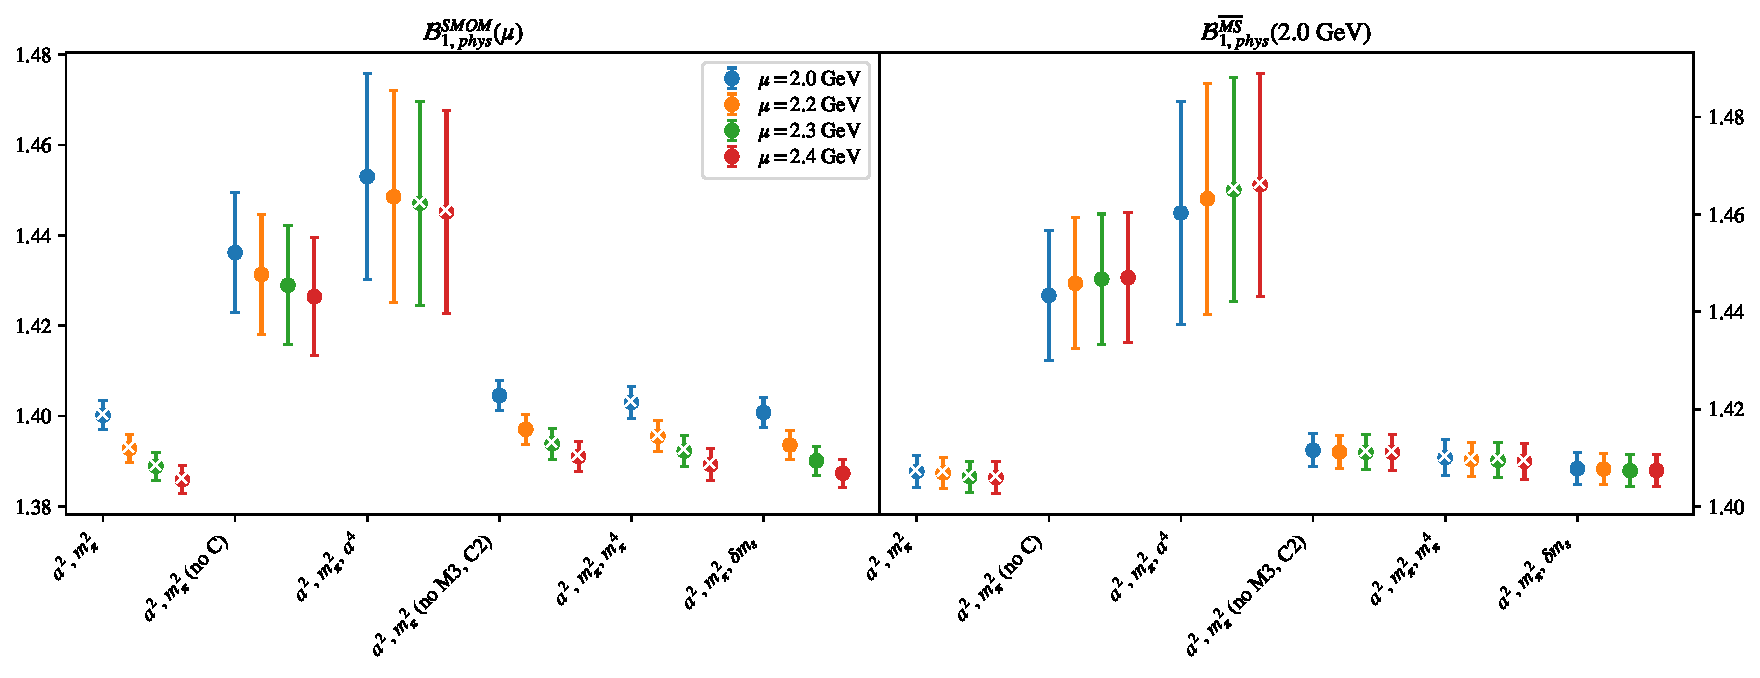
\includegraphics[page=1, width=1.1\textwidth]{VVpAA/NPR/fit_summary_bag.pdf}
\caption{$\mathcal{B}_{1}$\\(left) $\mathcal{B}_{phys}$ in RI/SMOM scheme from fit variations (fits with $p$-value $<0.05$ marked with ``$\times$"). \\(right) $\mathcal{B}_{phys}$ in $\overline{MS}$ computed using $\mathcal{B}^{\overline{MS}} = R^{\overline{MS}\leftarrow SMOM}(2.0)\sigma_{npt}(2.0,\mu) \mathcal{B}^{SMOM}(\mu)$.}
\end{figure}
\clearpage
\begin{figure}
\centering
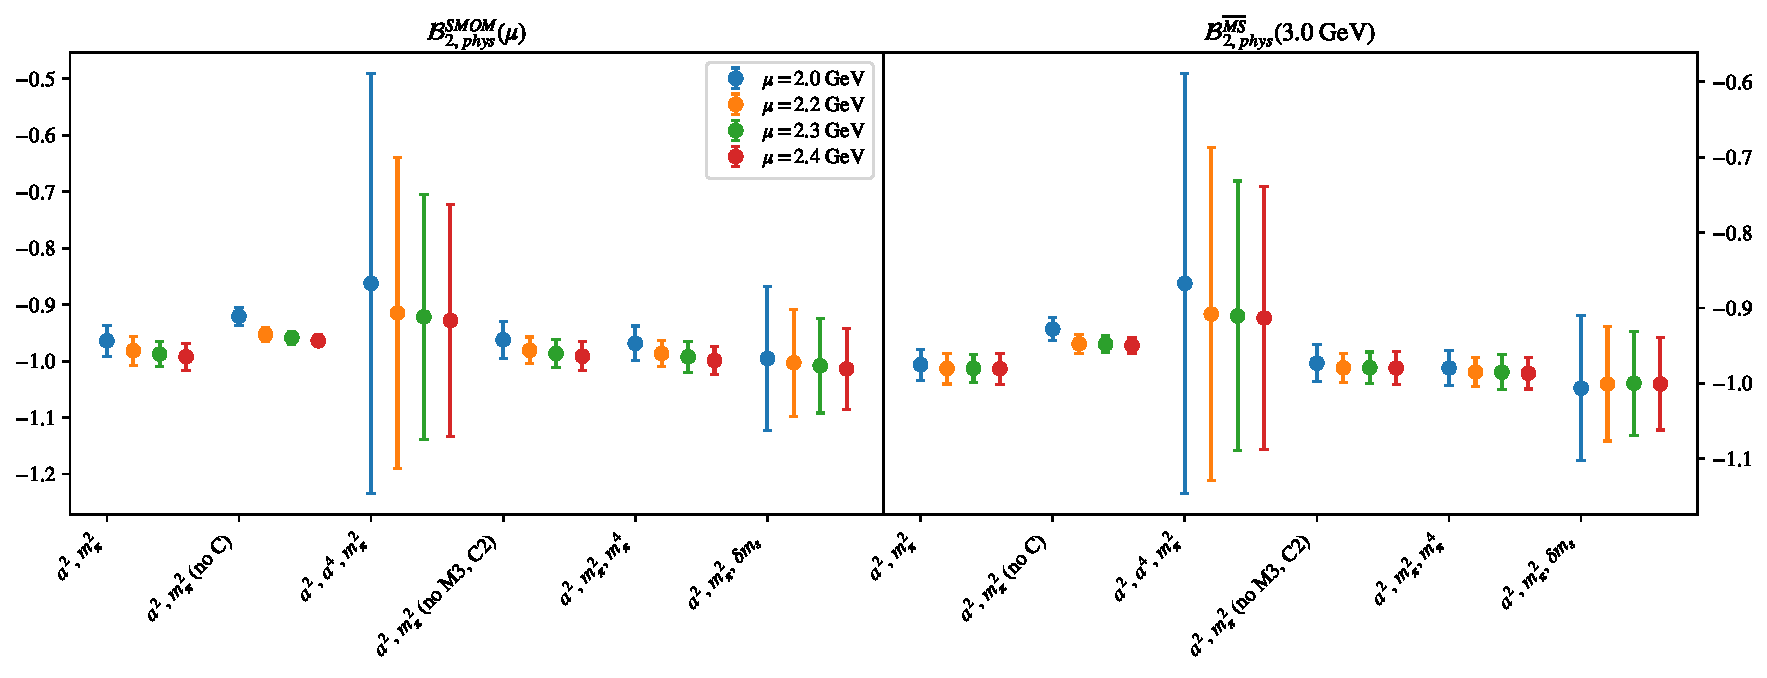
\includegraphics[page=1, width=1.1\textwidth]{VVmAA/NPR/fit_summary_bag.pdf}
\caption{$\mathcal{B}_{2}$\\(left) $\mathcal{B}_{phys}$ in RI/SMOM scheme from fit variations (fits with $p$-value $<0.05$ marked with ``$\times$"). \\(right) $\mathcal{B}_{phys}$ in $\overline{MS}$ computed using $\mathcal{B}^{\overline{MS}} = R^{\overline{MS}\leftarrow SMOM}(3.0)\sigma_{npt}(3.0,\mu) \mathcal{B}^{SMOM}(\mu)$.}
\end{figure}
\clearpage
\begin{figure}
\centering
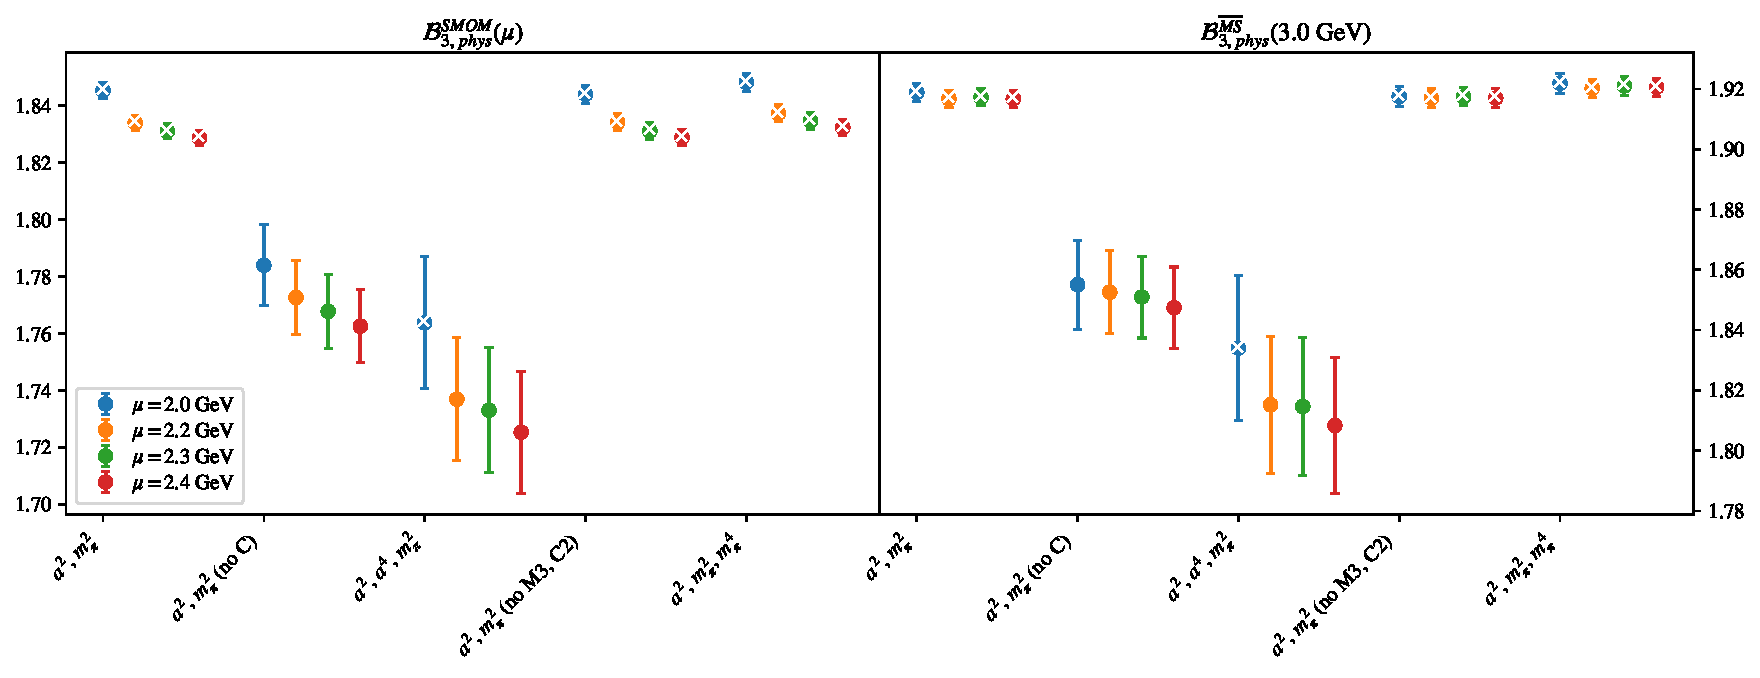
\includegraphics[page=1, width=1.1\textwidth]{SSmPP/NPR/fit_summary_bag.pdf}
\caption{$\mathcal{B}_{3}$\\(left) $\mathcal{B}_{phys}$ in RI/SMOM scheme from fit variations (fits with $p$-value $<0.05$ marked with ``$\times$"). \\(right) $\mathcal{B}_{phys}$ in $\overline{MS}$ computed using $\mathcal{B}^{\overline{MS}} = R^{\overline{MS}\leftarrow SMOM}(3.0)\sigma_{npt}(3.0,\mu) \mathcal{B}^{SMOM}(\mu)$.}
\end{figure}
\clearpage
\begin{figure}
\centering
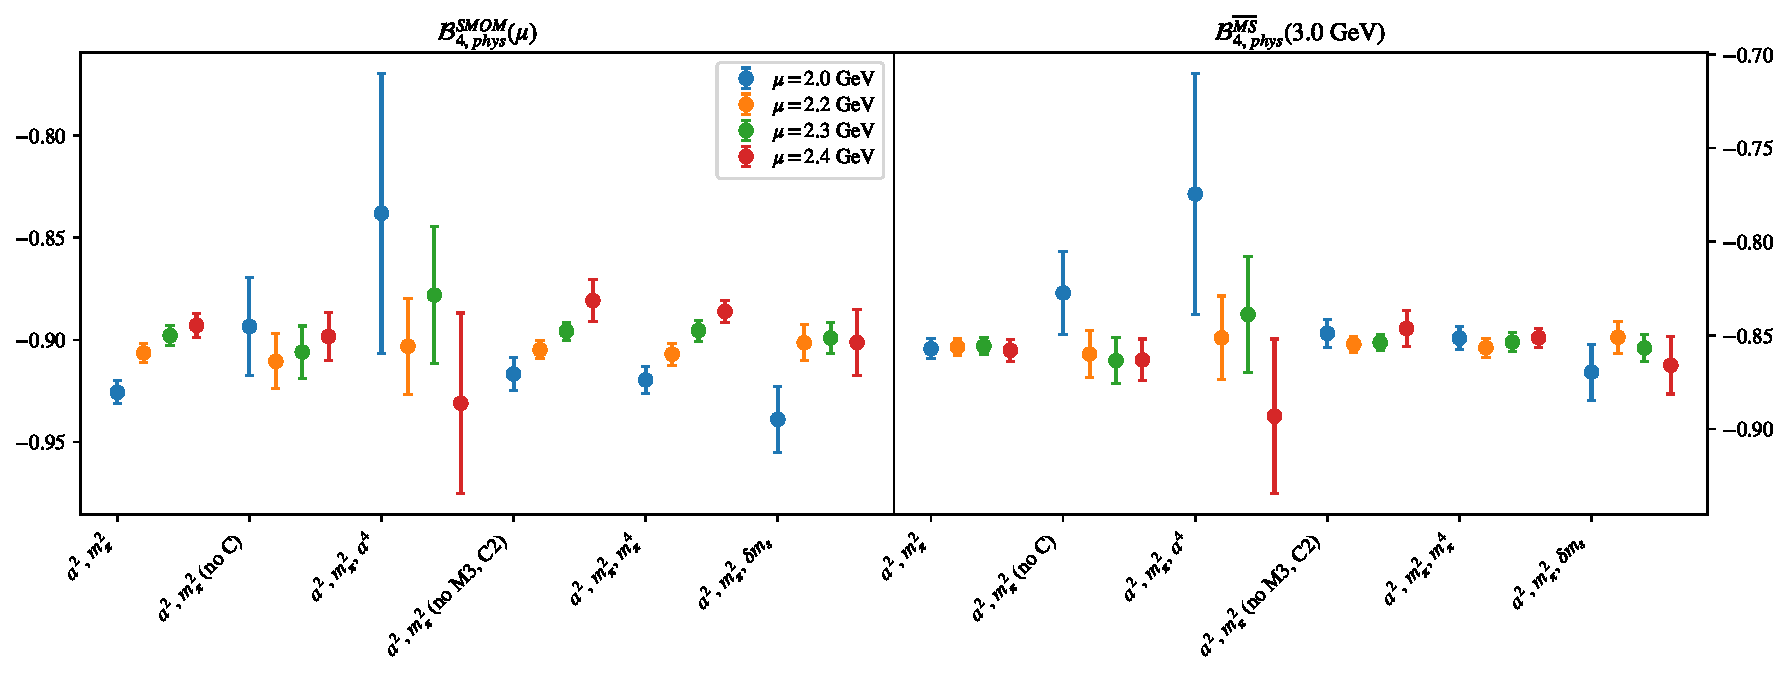
\includegraphics[page=1, width=1.1\textwidth]{SSpPP/NPR/fit_summary_bag.pdf}
\caption{$\mathcal{B}_{4}$\\(left) $\mathcal{B}_{phys}$ in RI/SMOM scheme from fit variations (fits with $p$-value $<0.05$ marked with ``$\times$"). \\(right) $\mathcal{B}_{phys}$ in $\overline{MS}$ computed using $\mathcal{B}^{\overline{MS}} = R^{\overline{MS}\leftarrow SMOM}(3.0)\sigma_{npt}(3.0,\mu) \mathcal{B}^{SMOM}(\mu)$.}
\end{figure}
\clearpage
\begin{figure}
\centering
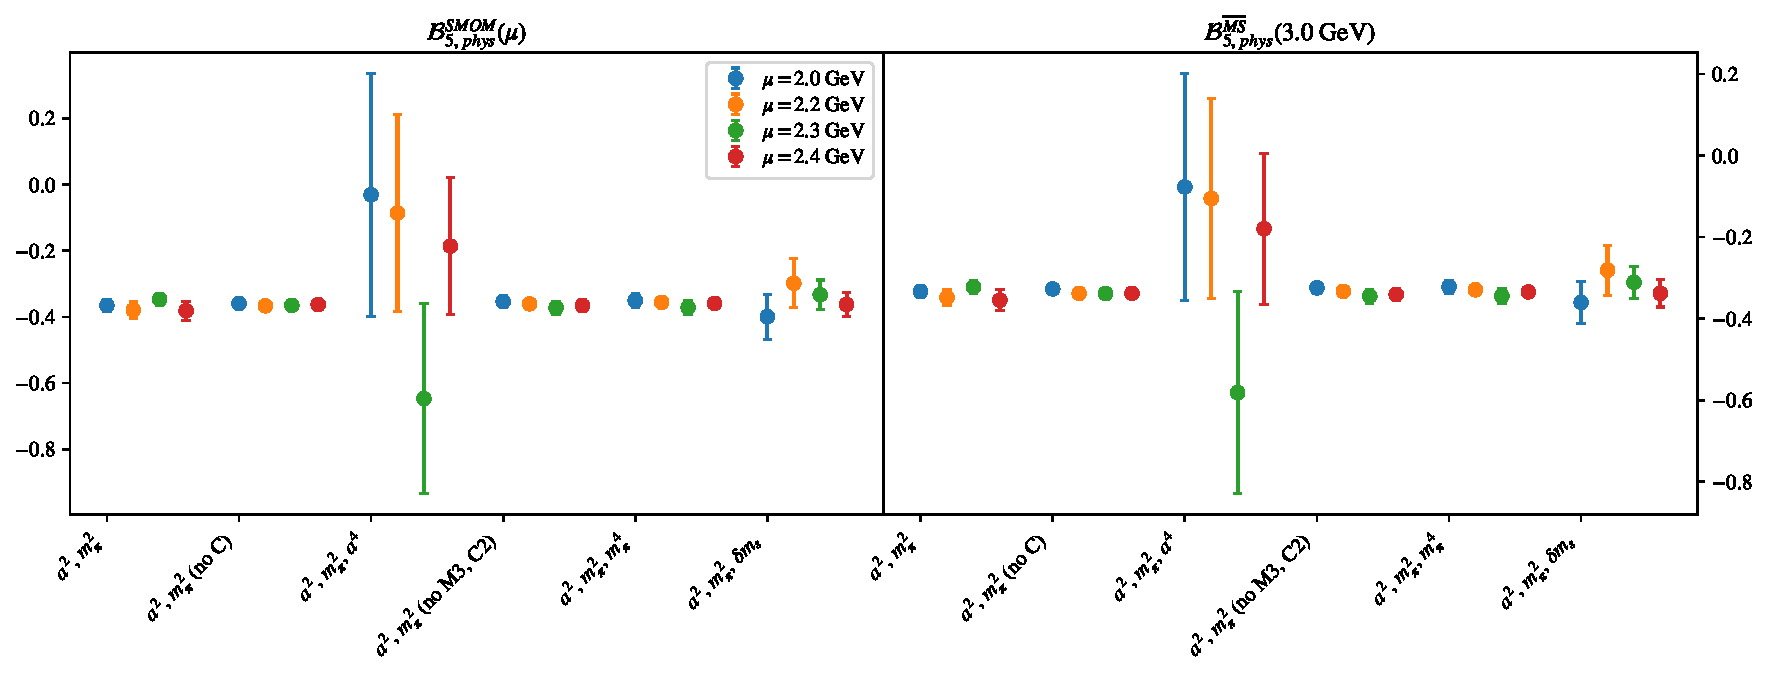
\includegraphics[page=1, width=1.1\textwidth]{TT/NPR/fit_summary_bag.pdf}
\caption{$\mathcal{B}_{5}$\\(left) $\mathcal{B}_{phys}$ in RI/SMOM scheme from fit variations (fits with $p$-value $<0.05$ marked with ``$\times$"). \\(right) $\mathcal{B}_{phys}$ in $\overline{MS}$ computed using $\mathcal{B}^{\overline{MS}} = R^{\overline{MS}\leftarrow SMOM}(3.0)\sigma_{npt}(3.0,\mu) \mathcal{B}^{SMOM}(\mu)$.}
\end{figure}
\clearpage
\section{$\mathcal{B}_1$}
\begin{table}[h!]
\begin{center}
\begin{tabular}{|c|c|c|c|c|c|c|}
\hline
$\mu$ (GeV) & $a^2$, $m_\pi^2$& $a^2$, $m_\pi^2$ (no C)& $a^2$, $m_\pi^2$, $a^4$& $a^2$, $m_\pi^2$ (no M3, C2)& $a^2$, $m_\pi^2$, $m_\pi^4$& $a^2$, $m_\pi^2$, $\delta m_s$\\
\hline
2.0& \hyperlink{VVpAA/NPR/bag_a2m2_20.pdf.1}{\textbf{1.4002(32)}: 2.608 (0.023)} & \hyperlink{VVpAA/NPR/bag_a2m2noC_20.pdf.1}{\textbf{1.436(13)}: 0.273 (0.761)} & \hyperlink{VVpAA/NPR/bag_a2a4m2_20.pdf.1}{\textbf{1.453(22)}: 2.097 (0.078)} & \hyperlink{VVpAA/NPR/bag_a2m2mcut_20.pdf.1}{\textbf{1.4046(33)}: 2.257 (0.08)} & \hyperlink{VVpAA/NPR/bag_a2m2m4_20.pdf.1}{\textbf{1.4031(35)}: 2.755 (0.026)} & \hyperlink{VVpAA/NPR/bag_a2m2delm_20.pdf.1}{\textbf{1.4008(32)}: 1.363 (0.244)}\\
2.2& \hyperlink{VVpAA/NPR/bag_a2m2_22.pdf.1}{\textbf{1.3928(31)}: 3.087 (0.009)} & \hyperlink{VVpAA/NPR/bag_a2m2noC_22.pdf.1}{\textbf{1.431(13)}: 0.303 (0.739)} & \hyperlink{VVpAA/NPR/bag_a2a4m2_22.pdf.1}{\textbf{1.449(23)}: 2.242 (0.062)} & \hyperlink{VVpAA/NPR/bag_a2m2mcut_22.pdf.1}{\textbf{1.3971(32)}: 2.457 (0.061)} & \hyperlink{VVpAA/NPR/bag_a2m2m4_22.pdf.1}{\textbf{1.3956(34)}: 3.145 (0.014)} & \hyperlink{VVpAA/NPR/bag_a2m2delm_22.pdf.1}{\textbf{1.3936(31)}: 1.453 (0.214)}\\
2.3& \hyperlink{VVpAA/NPR/bag_a2m2_23.pdf.1}{\textbf{1.3889(31)}: 3.371 (0.005)} & \hyperlink{VVpAA/NPR/bag_a2m2noC_23.pdf.1}{\textbf{1.429(13)}: 0.338 (0.713)} & \hyperlink{VVpAA/NPR/bag_a2a4m2_23.pdf.1}{\textbf{1.447(22)}: 2.555 (0.037)} & \hyperlink{VVpAA/NPR/bag_a2m2mcut_23.pdf.1}{\textbf{1.3939(34)}: 2.644 (0.047)} & \hyperlink{VVpAA/NPR/bag_a2m2m4_23.pdf.1}{\textbf{1.3923(35)}: 3.247 (0.011)} & \hyperlink{VVpAA/NPR/bag_a2m2delm_23.pdf.1}{\textbf{1.3901(31)}: 1.606 (0.17)}\\
2.4& \hyperlink{VVpAA/NPR/bag_a2m2_24.pdf.1}{\textbf{1.3860(30)}: 3.577 (0.003)} & \hyperlink{VVpAA/NPR/bag_a2m2noC_24.pdf.1}{\textbf{1.426(13)}: 0.341 (0.711)} & \hyperlink{VVpAA/NPR/bag_a2a4m2_24.pdf.1}{\textbf{1.445(22)}: 2.727 (0.028)} & \hyperlink{VVpAA/NPR/bag_a2m2mcut_24.pdf.1}{\textbf{1.3911(34)}: 2.749 (0.041)} & \hyperlink{VVpAA/NPR/bag_a2m2m4_24.pdf.1}{\textbf{1.3893(35)}: 3.38 (0.009)} & \hyperlink{VVpAA/NPR/bag_a2m2delm_24.pdf.1}{\textbf{1.3874(31)}: 1.611 (0.168)}\\
\hline
\end{tabular}
\caption{Physical point value from chiral and continuum extrapolation at renormalisation scale $\mu$. Entries are \textbf{value(error)}: $\chi^2/\text{DOF}$ ($p$-value).}
\end{center}
\end{table}
\begin{table}[h!]
\begin{center}
\begin{tabular}{|c c|c|c|c|c|c|c|}
\hline
$\mu$ (GeV) &  & $a^2$, $m_\pi^2$& $a^2$, $m_\pi^2$ (no C)& $a^2$, $m_\pi^2$, $a^4$& $a^2$, $m_\pi^2$ (no M3, C2)& $a^2$, $m_\pi^2$, $m_\pi^4$& $a^2$, $m_\pi^2$, $\delta m_s$\\
\hline
\multirow{3}{0.5in}{2.0} & $\alpha$ & 0.147(11)& -0.055(78)& -0.34(20)& 0.133(12)& 0.139(12)& 0.150(11)\\
 & $\beta$ & 0.00409(21)& 0.00347(43)& 0.00435(23)& 0.00338(34)& 0.0023(10)& 0.00540(52)\\
 & $\gamma$ &  &  & 0.99(42)&  & 0.000157(95)& -0.052(19)\\
\hline
\multirow{3}{0.5in}{2.2} & $\alpha$ & 0.152(11)& -0.065(77)& -0.36(21)& 0.138(11)& 0.144(12)& 0.154(11)\\
 & $\beta$ & 0.00397(21)& 0.00331(41)& 0.00427(24)& 0.00327(34)& 0.0020(10)& 0.00539(52)\\
 & $\gamma$ &  &  & 1.04(43)&  & 0.000179(92)& -0.055(18)\\
\hline
\multirow{3}{0.5in}{2.3} & $\alpha$ & 0.155(10)& -0.068(77)& -0.38(20)& 0.140(12)& 0.145(12)& 0.157(11)\\
 & $\beta$ & 0.00394(21)& 0.00327(40)& 0.00422(24)& 0.00322(35)& 0.0020(10)& 0.00542(51)\\
 & $\gamma$ &  &  & 1.08(42)&  & 0.000176(91)& -0.057(18)\\
\hline
\multirow{3}{0.5in}{2.4} & $\alpha$ & 0.157(10)& -0.070(77)& -0.39(20)& 0.140(12)& 0.147(12)& 0.157(11)\\
 & $\beta$ & 0.00392(20)& 0.00323(40)& 0.00423(24)& 0.00318(34)& 0.0019(10)& 0.00538(51)\\
 & $\gamma$ &  &  & 1.11(42)&  & 0.000185(92)& -0.056(18)\\
\hline
\end{tabular}
\caption{Fit values of coefficients in $Q = Q_{phys} + \mathbf{\alpha} a^2 + \mathbf{\beta}\left(\frac{m_\pi^2}{f_\pi^2}-\frac{m_{\pi,PDG}^2}{f_\pi^2}\right) + \gamma(\ldots)$}
\end{center}
\end{table}
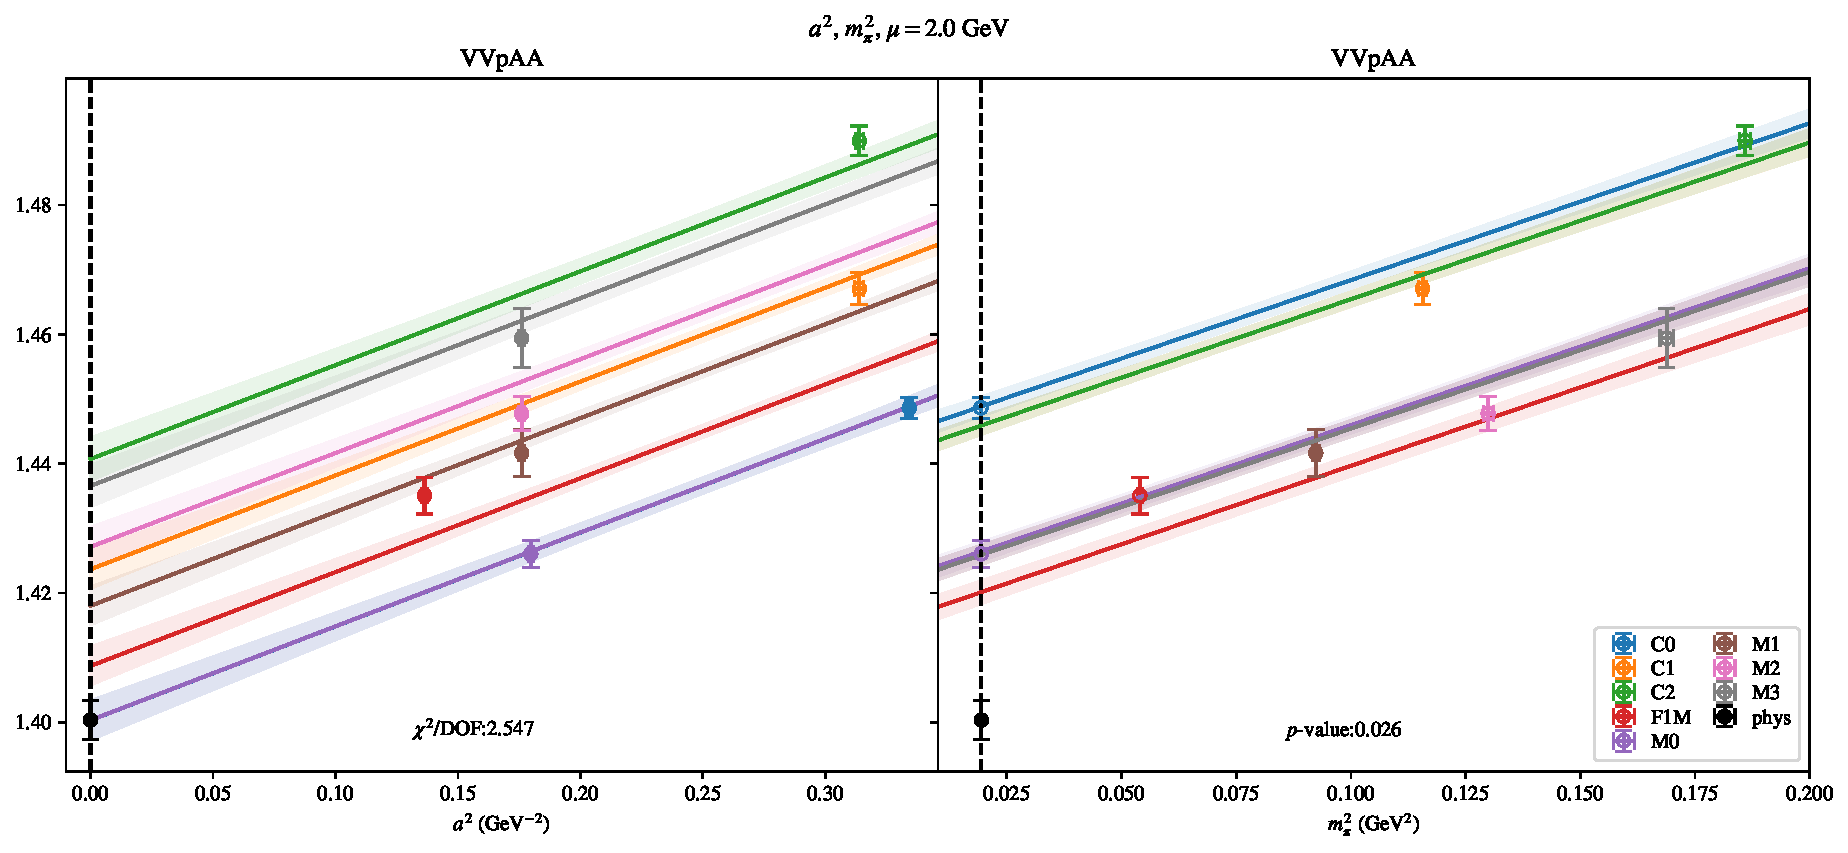
\includepdf[link, pages=-]{VVpAA/NPR/bag_a2m2_20.pdf}
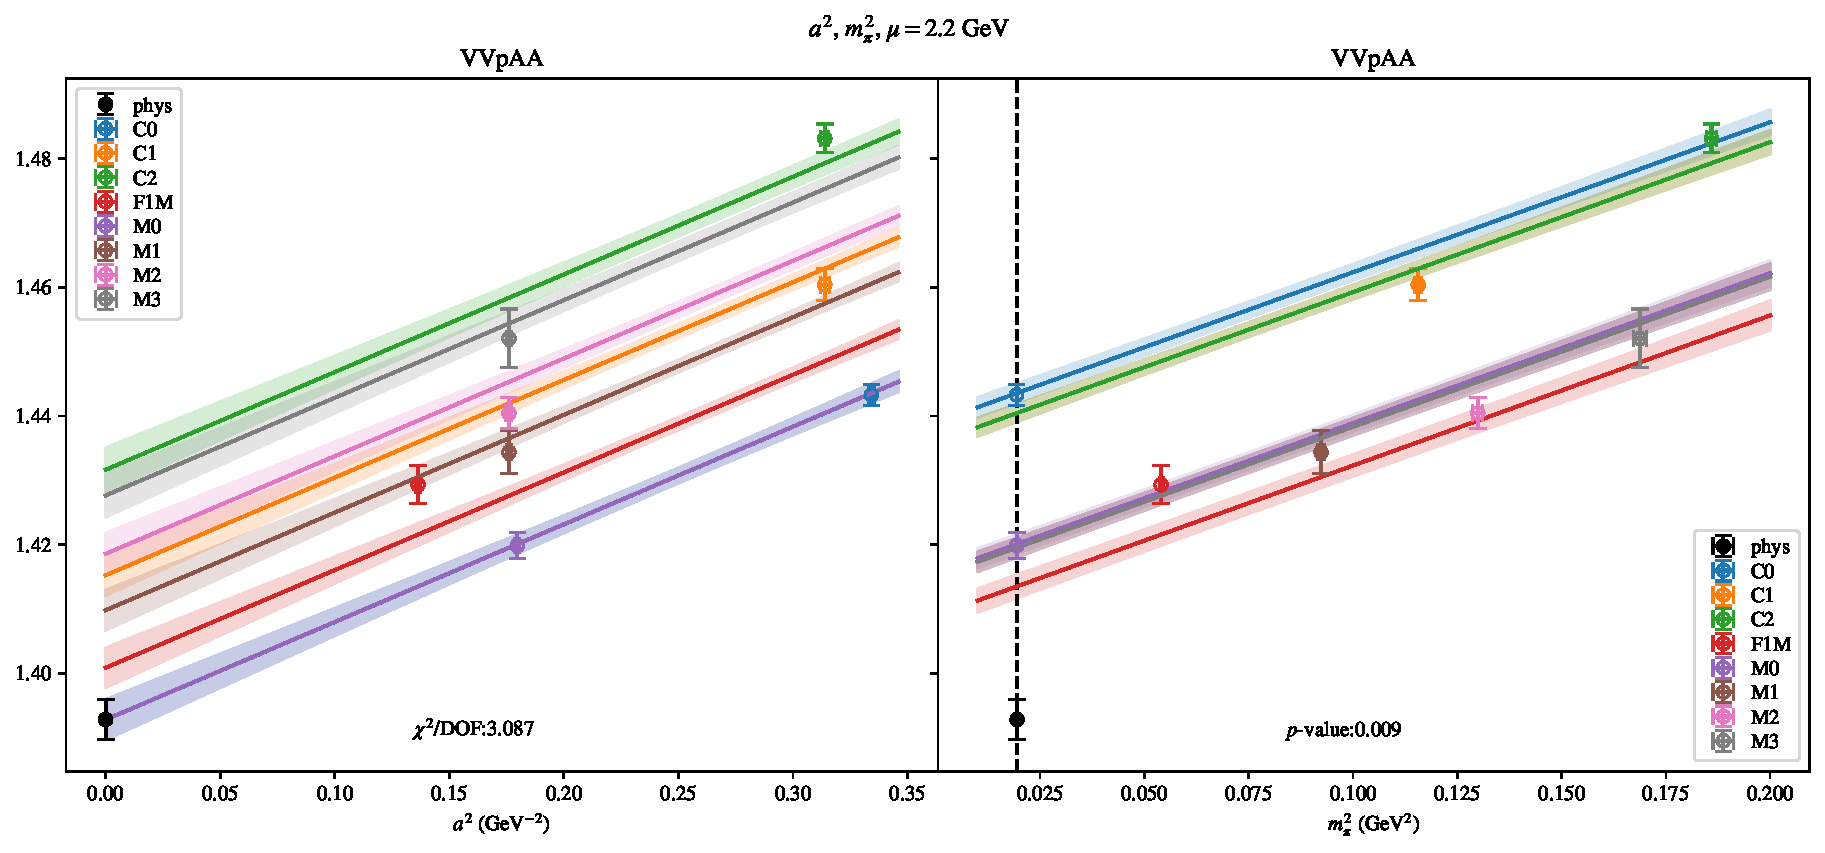
\includepdf[link, pages=-]{VVpAA/NPR/bag_a2m2_22.pdf}
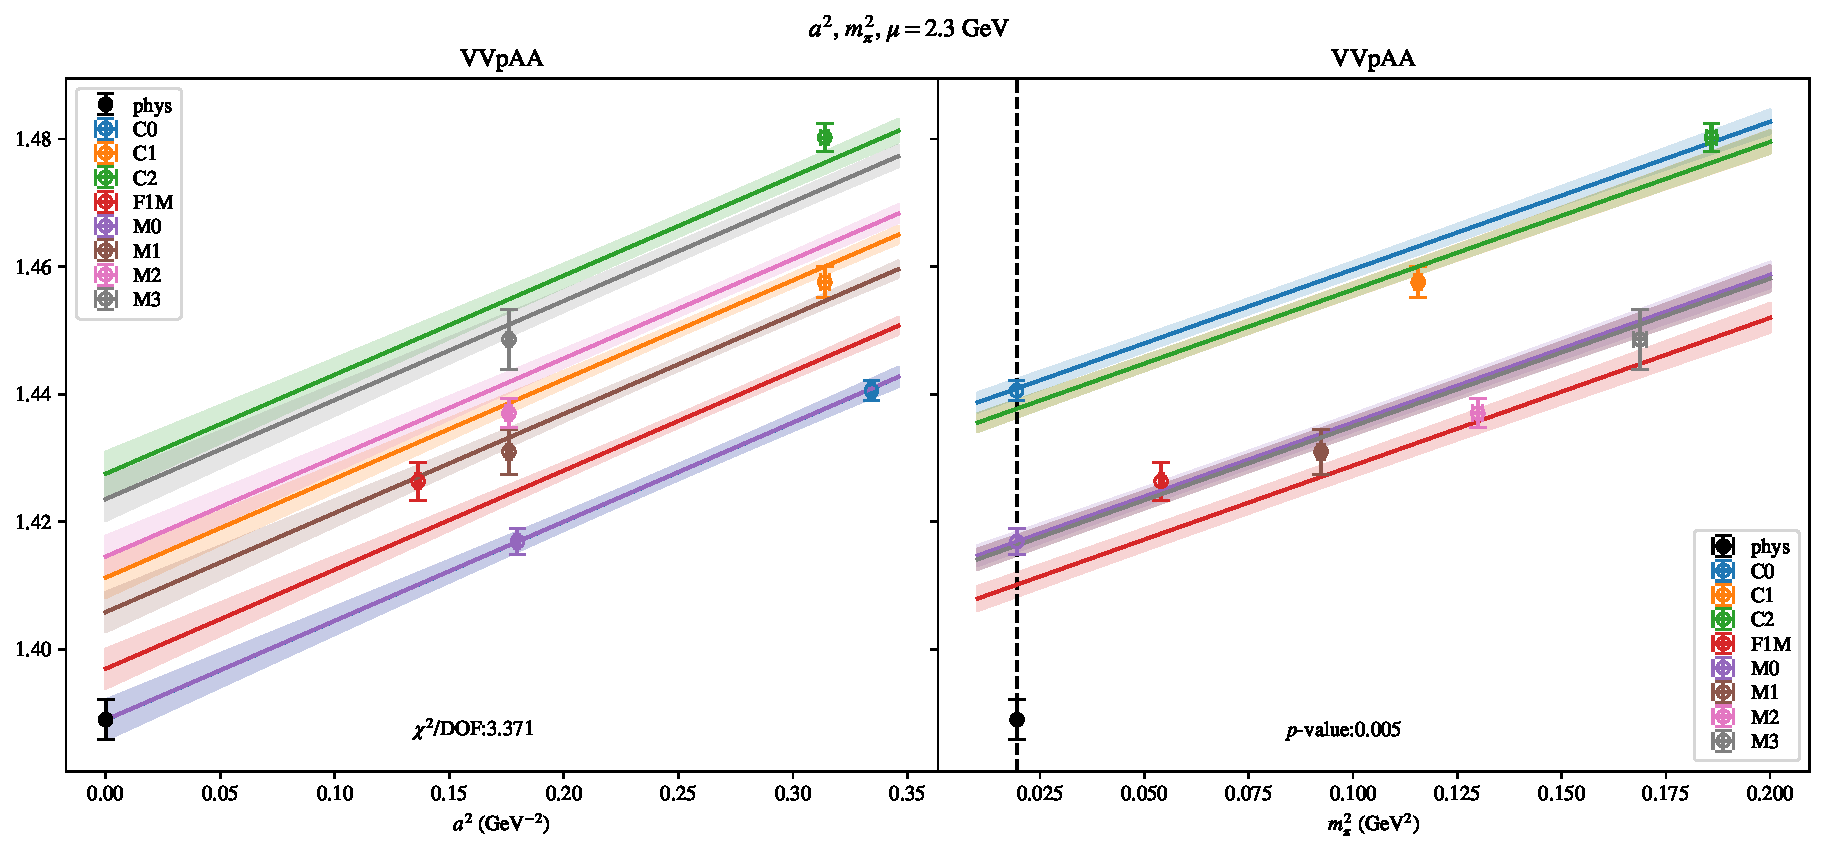
\includepdf[link, pages=-]{VVpAA/NPR/bag_a2m2_23.pdf}
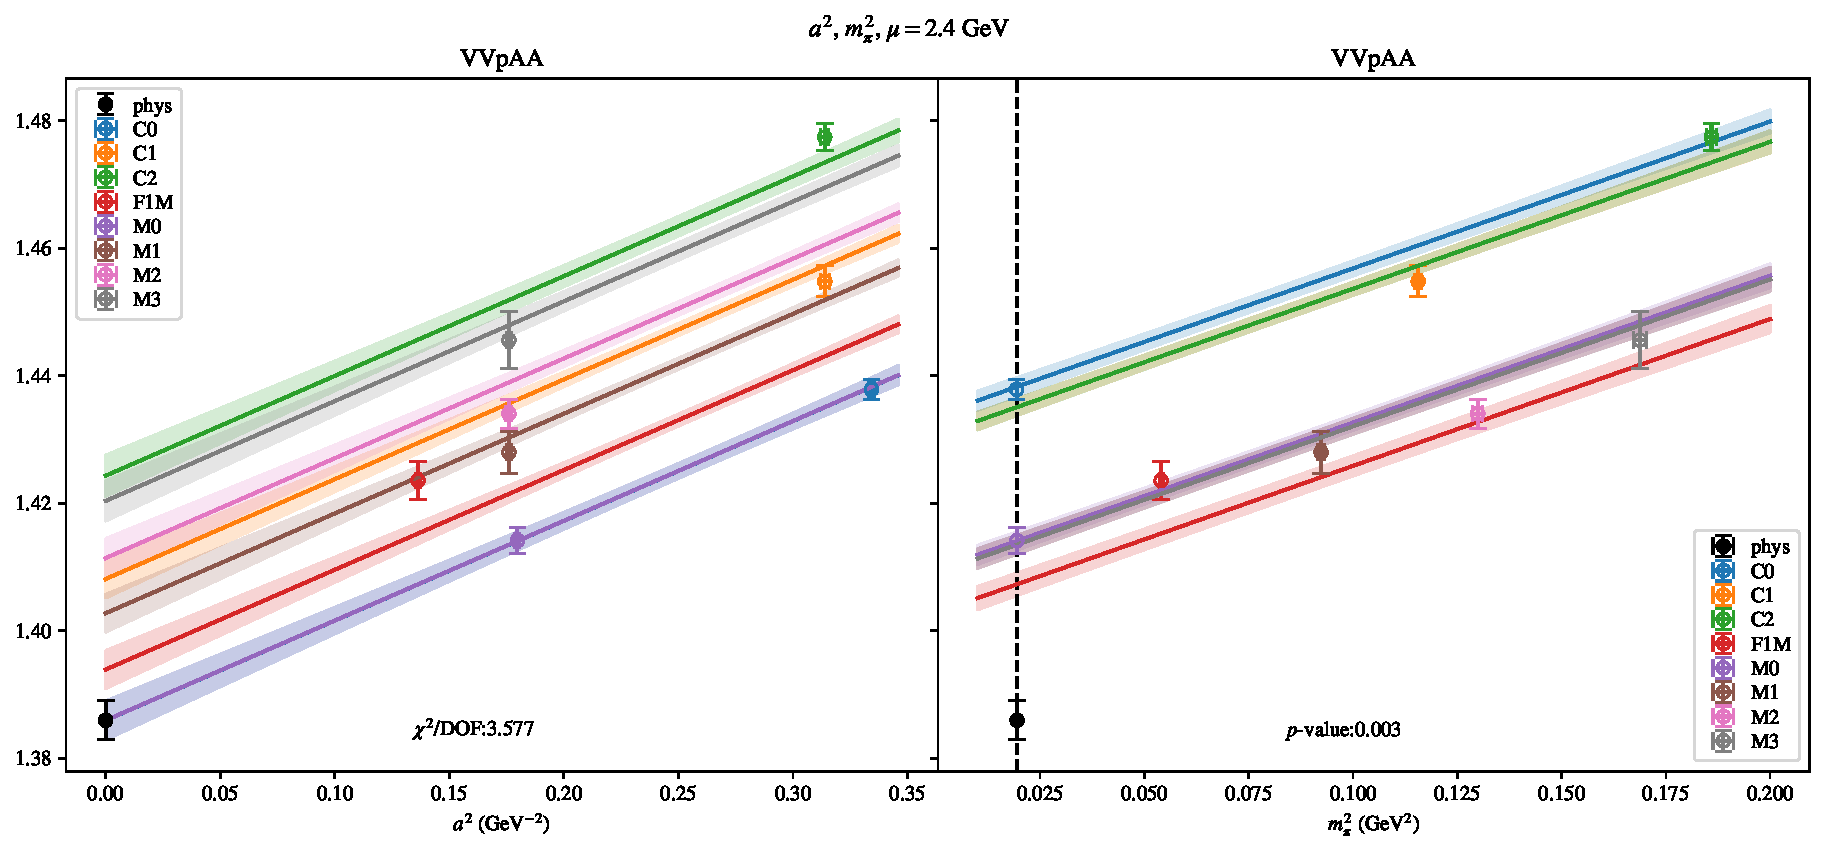
\includepdf[link, pages=-]{VVpAA/NPR/bag_a2m2_24.pdf}
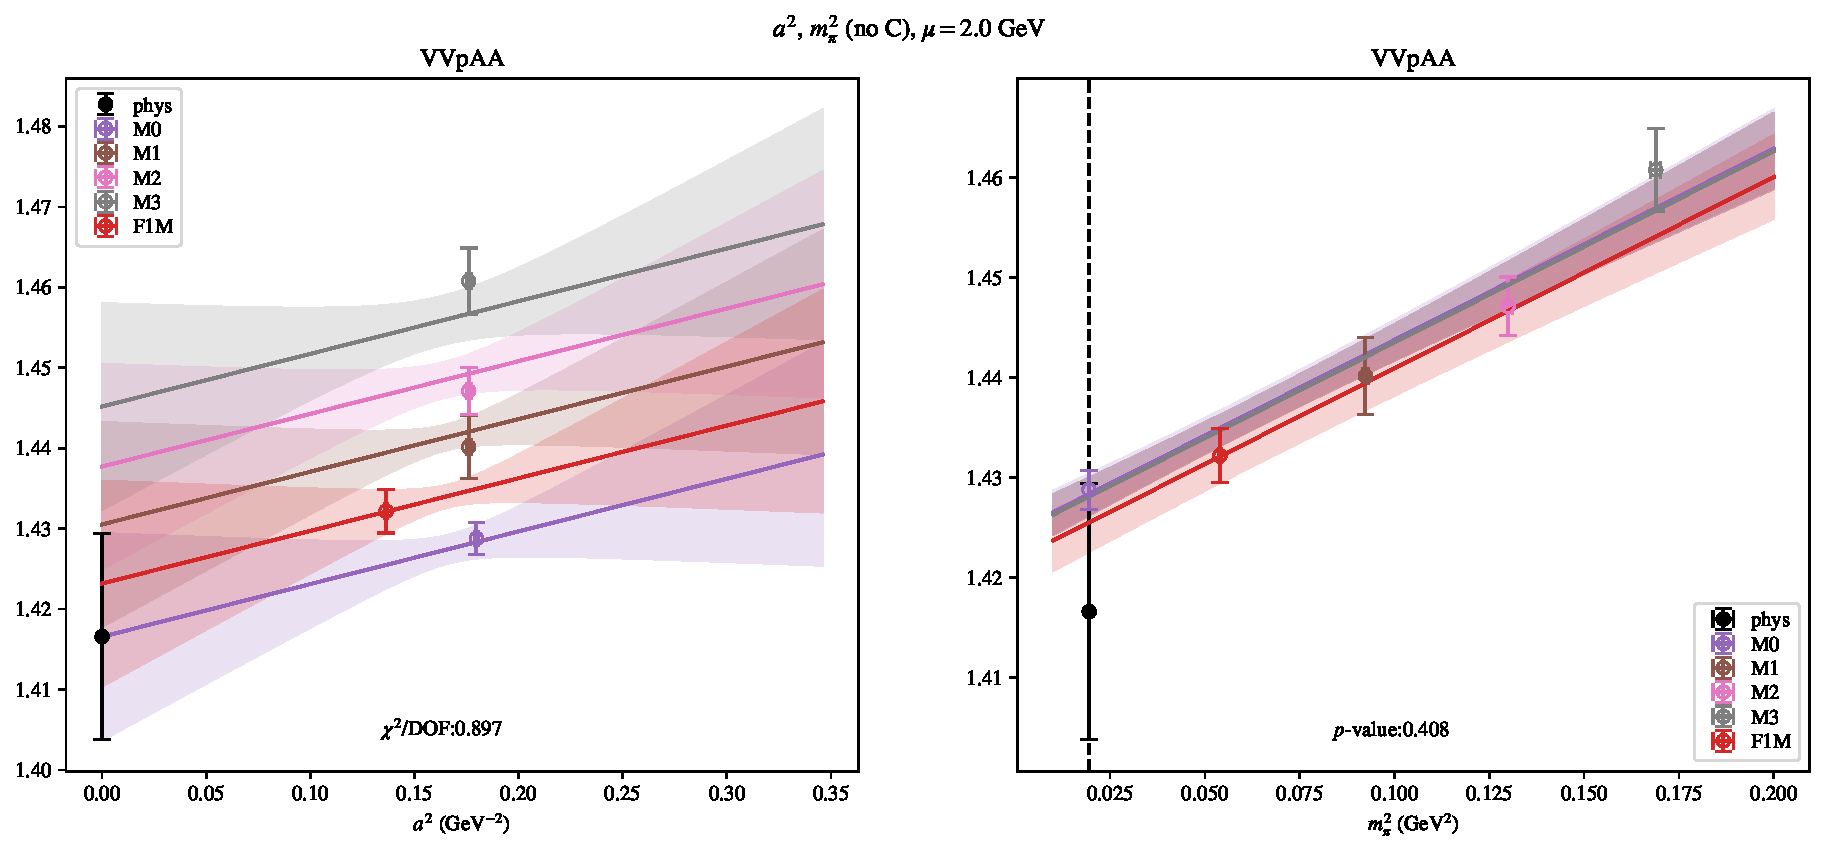
\includepdf[link, pages=-]{VVpAA/NPR/bag_a2m2noC_20.pdf}
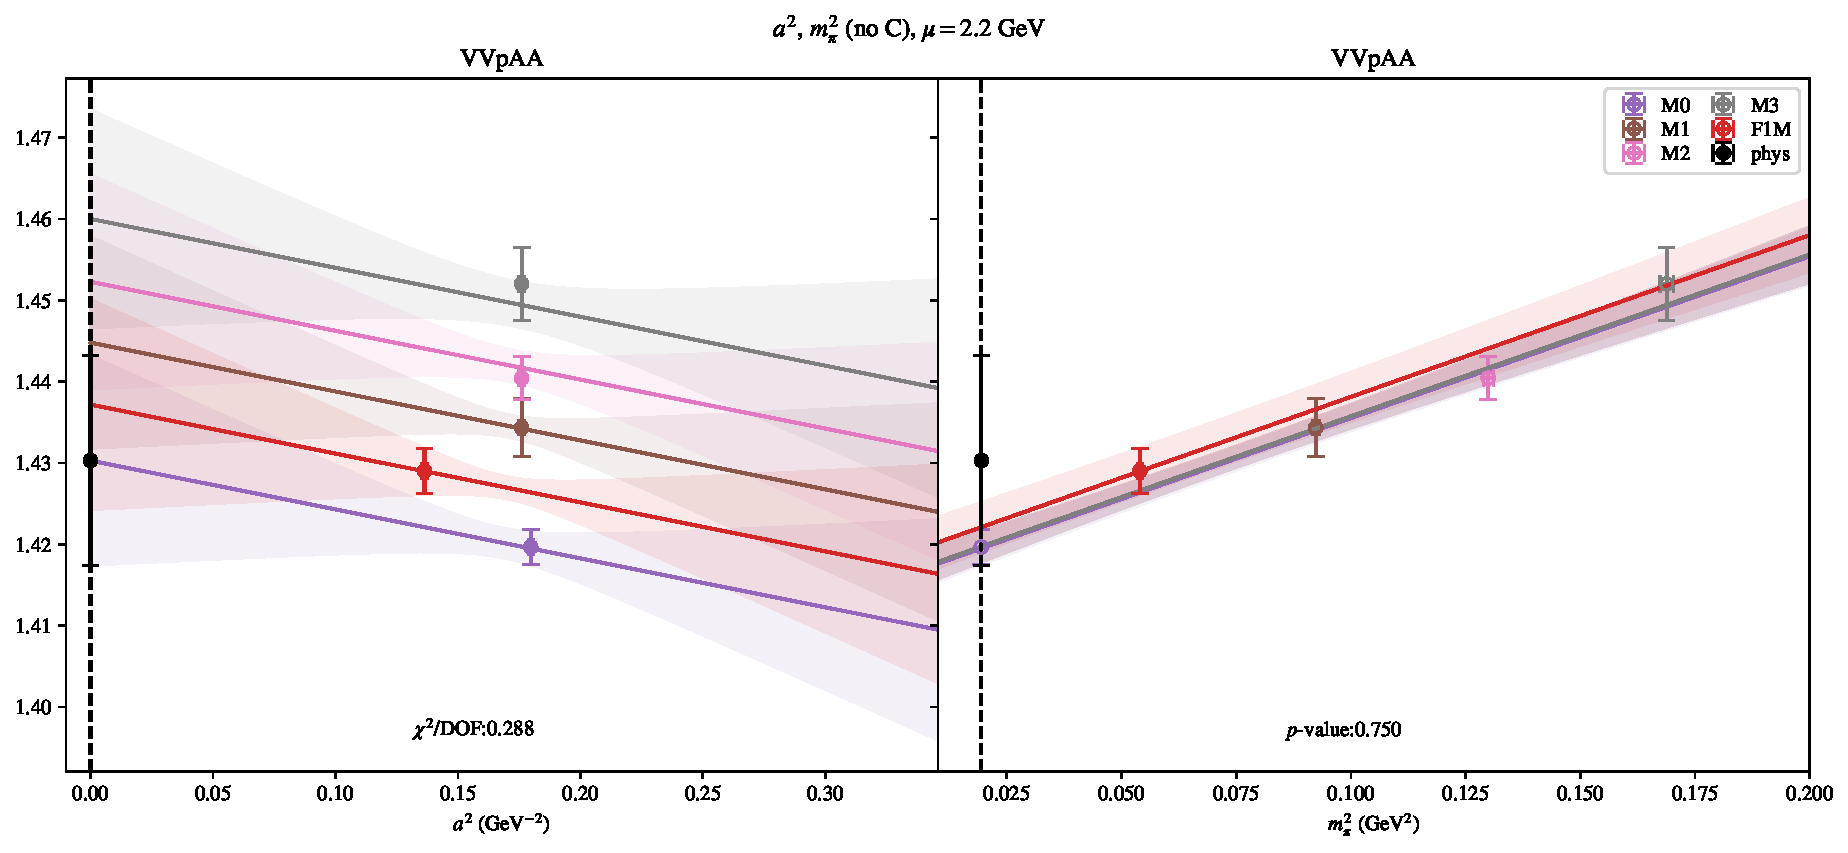
\includepdf[link, pages=-]{VVpAA/NPR/bag_a2m2noC_22.pdf}
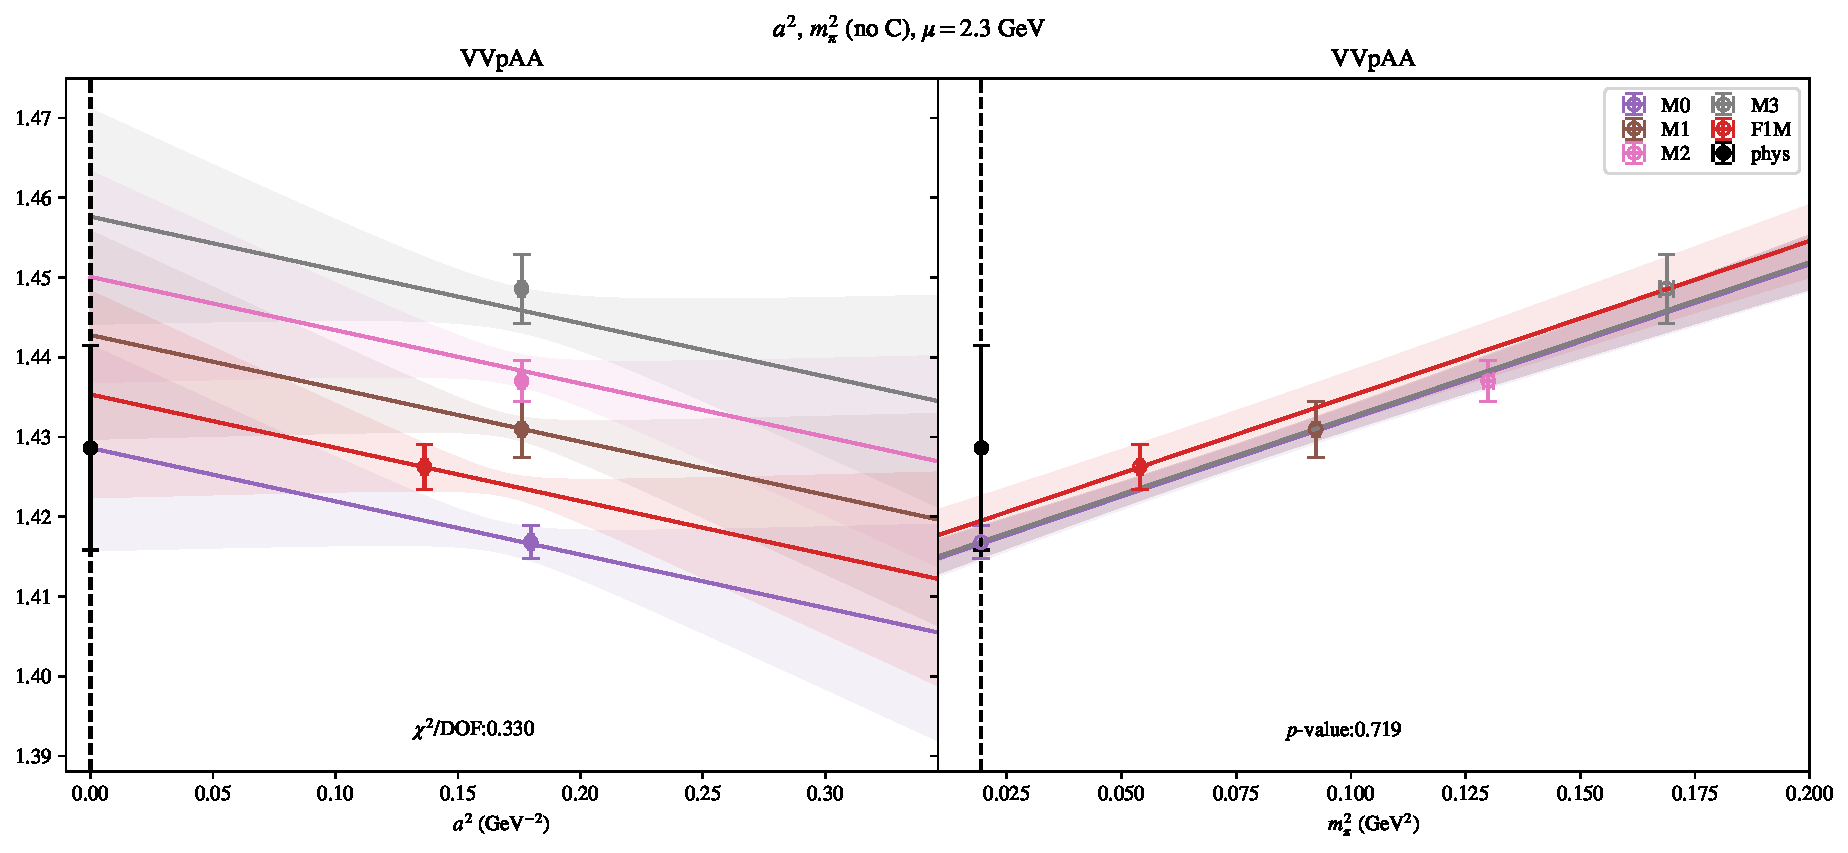
\includepdf[link, pages=-]{VVpAA/NPR/bag_a2m2noC_23.pdf}
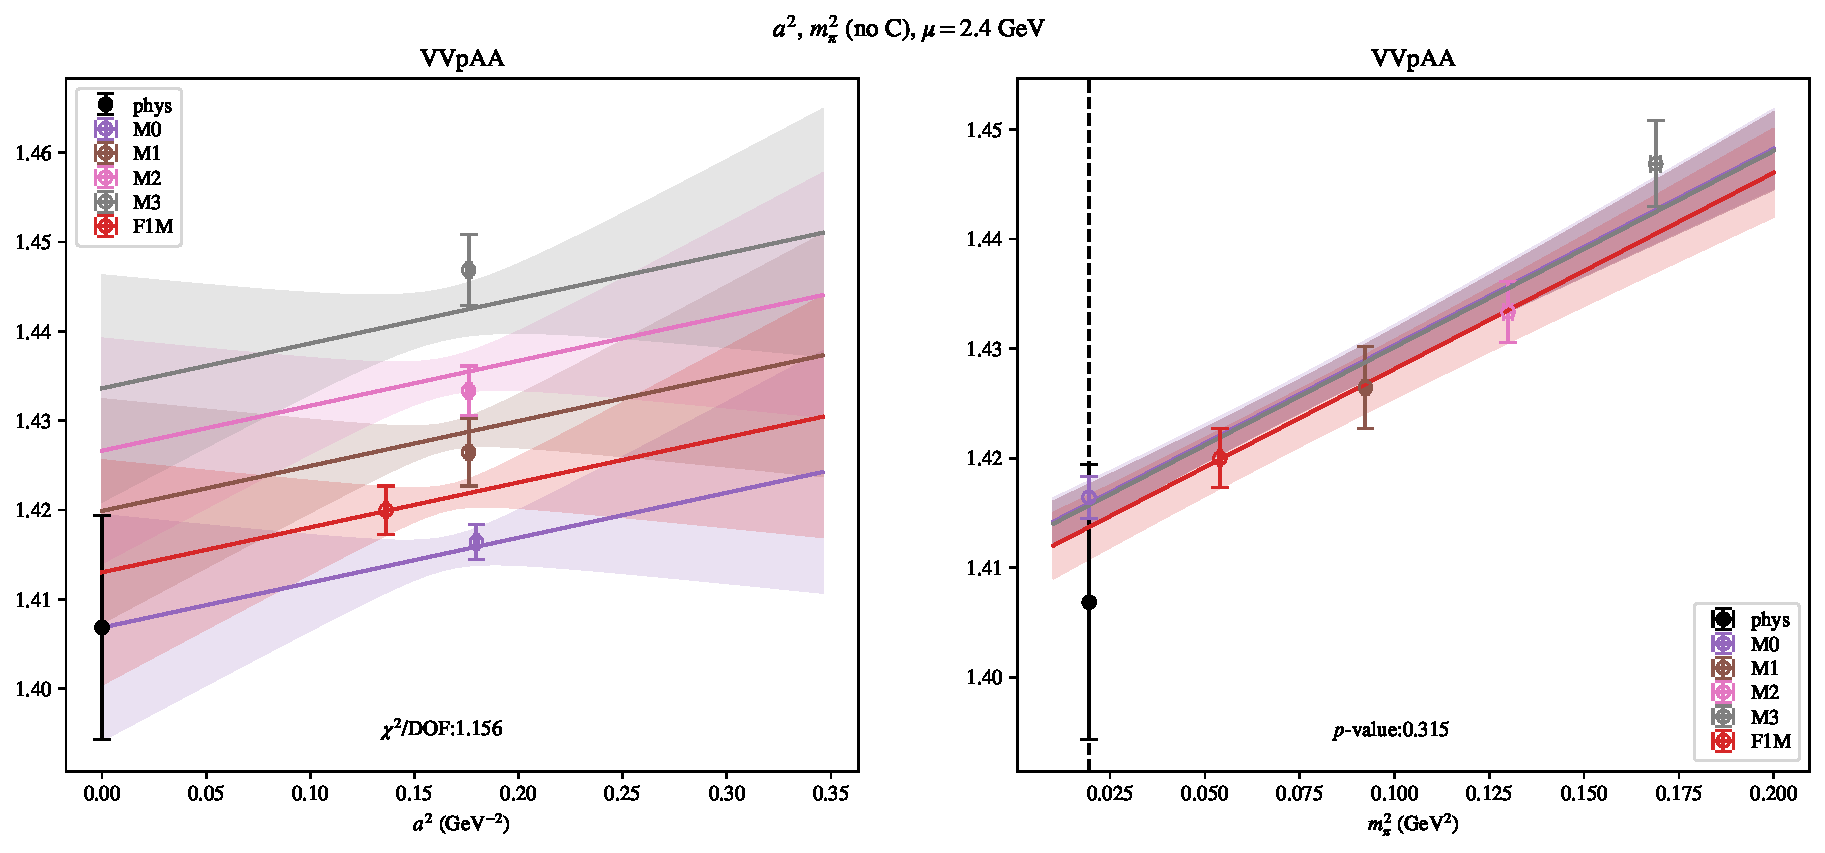
\includepdf[link, pages=-]{VVpAA/NPR/bag_a2m2noC_24.pdf}
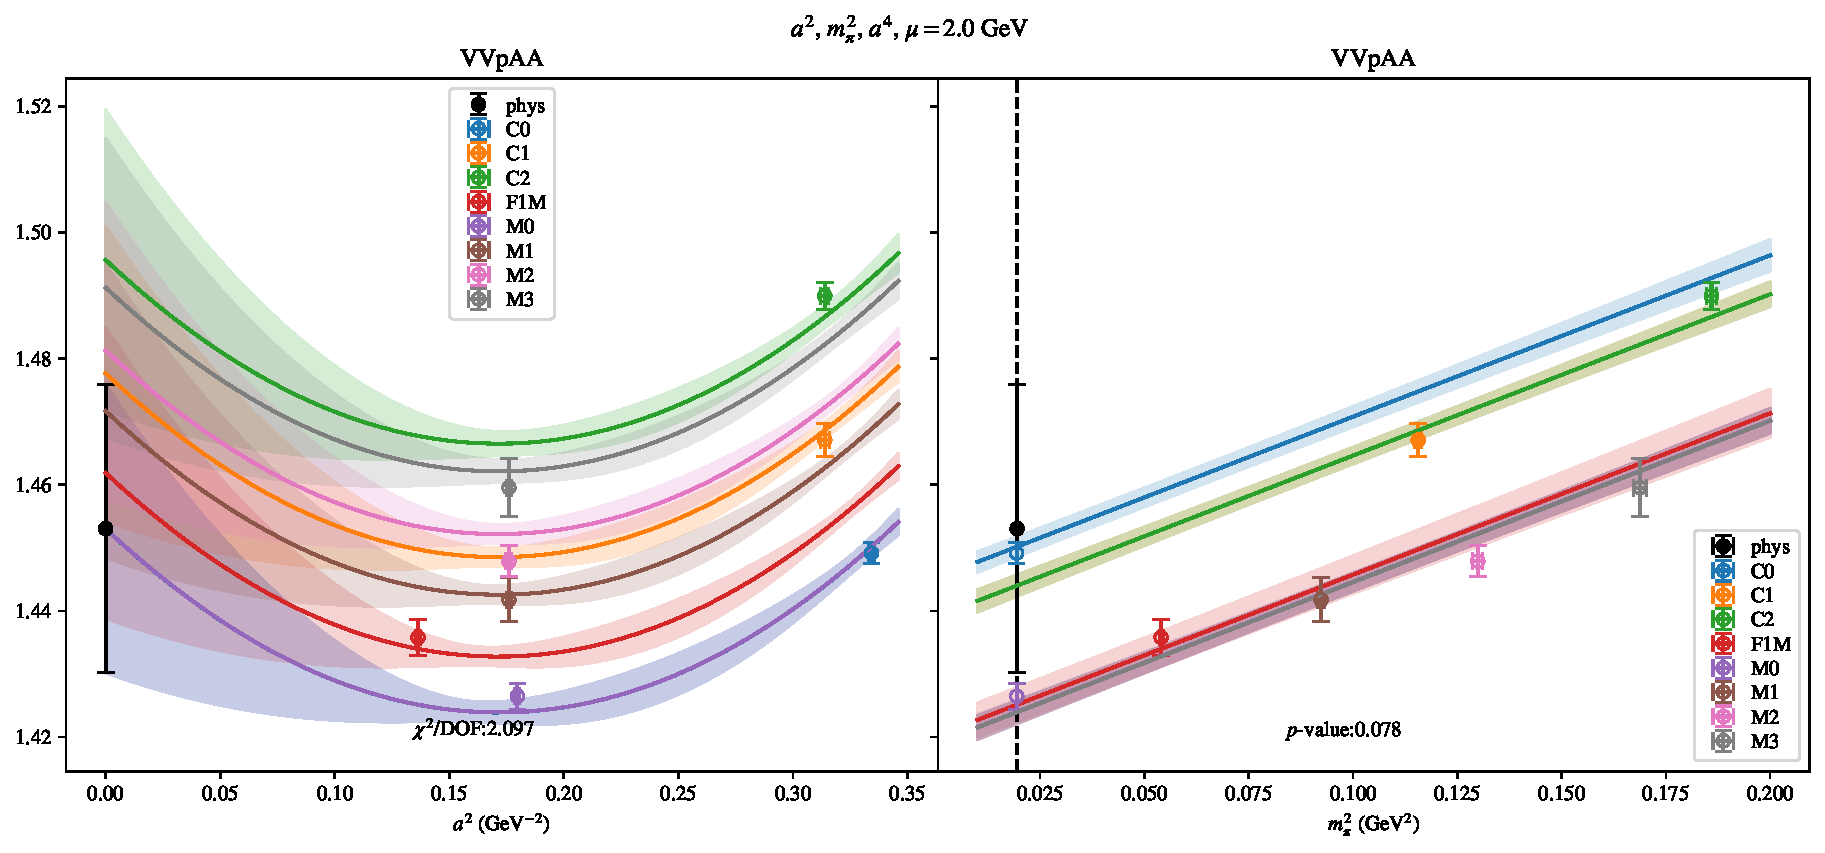
\includepdf[link, pages=-]{VVpAA/NPR/bag_a2a4m2_20.pdf}
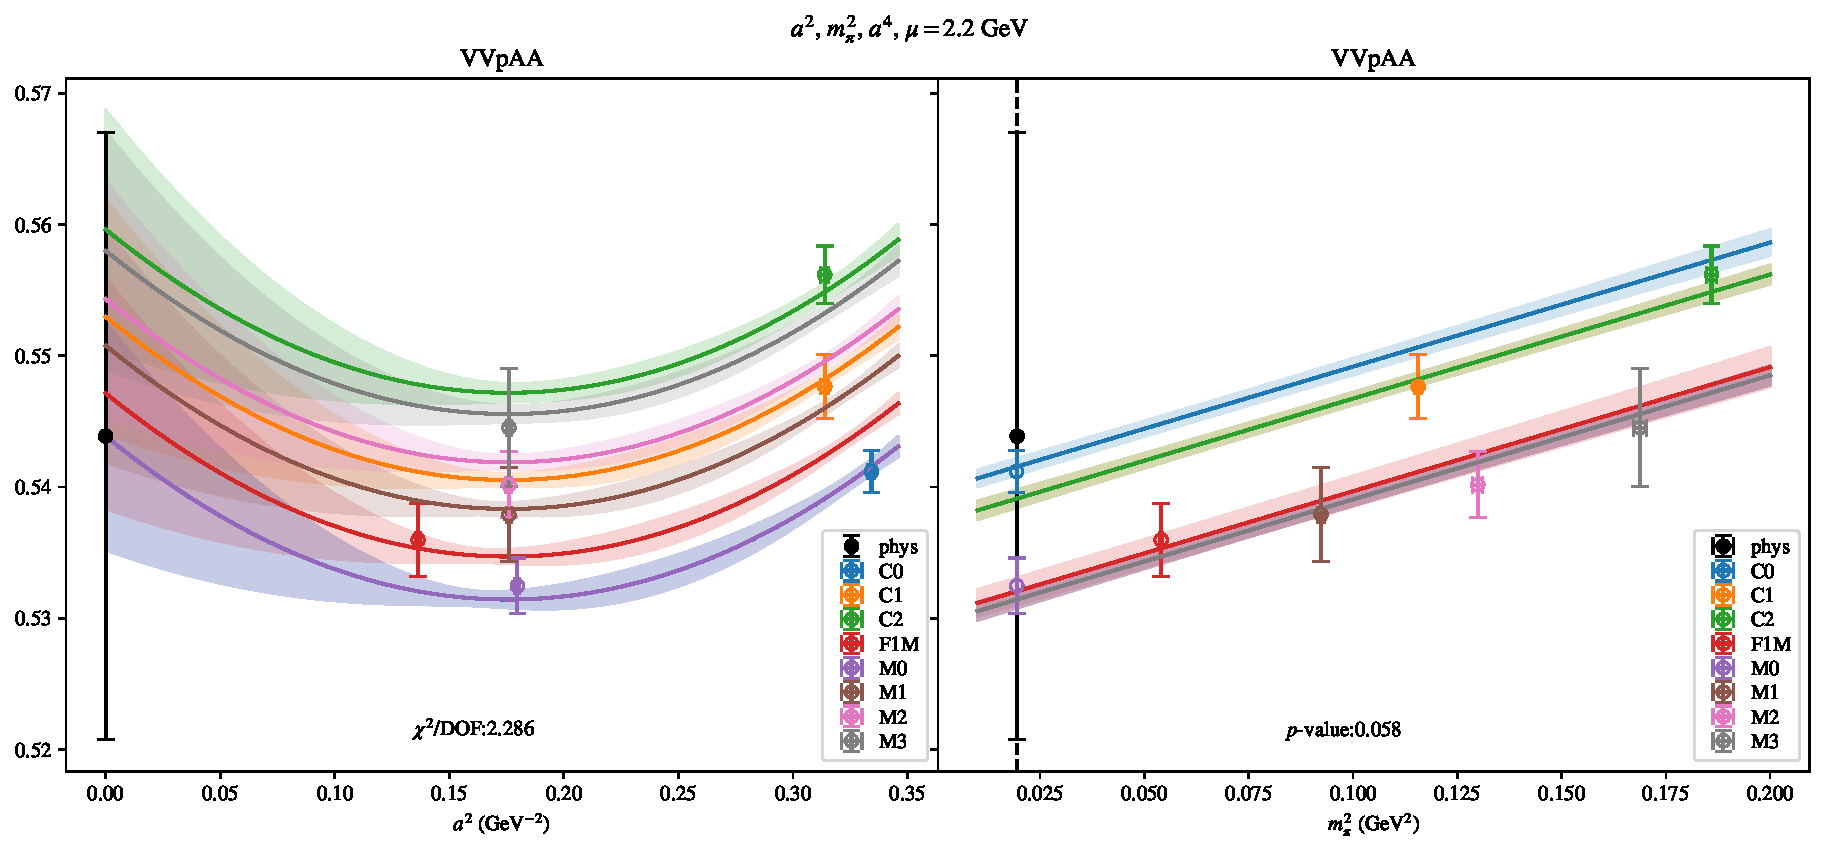
\includepdf[link, pages=-]{VVpAA/NPR/bag_a2a4m2_22.pdf}
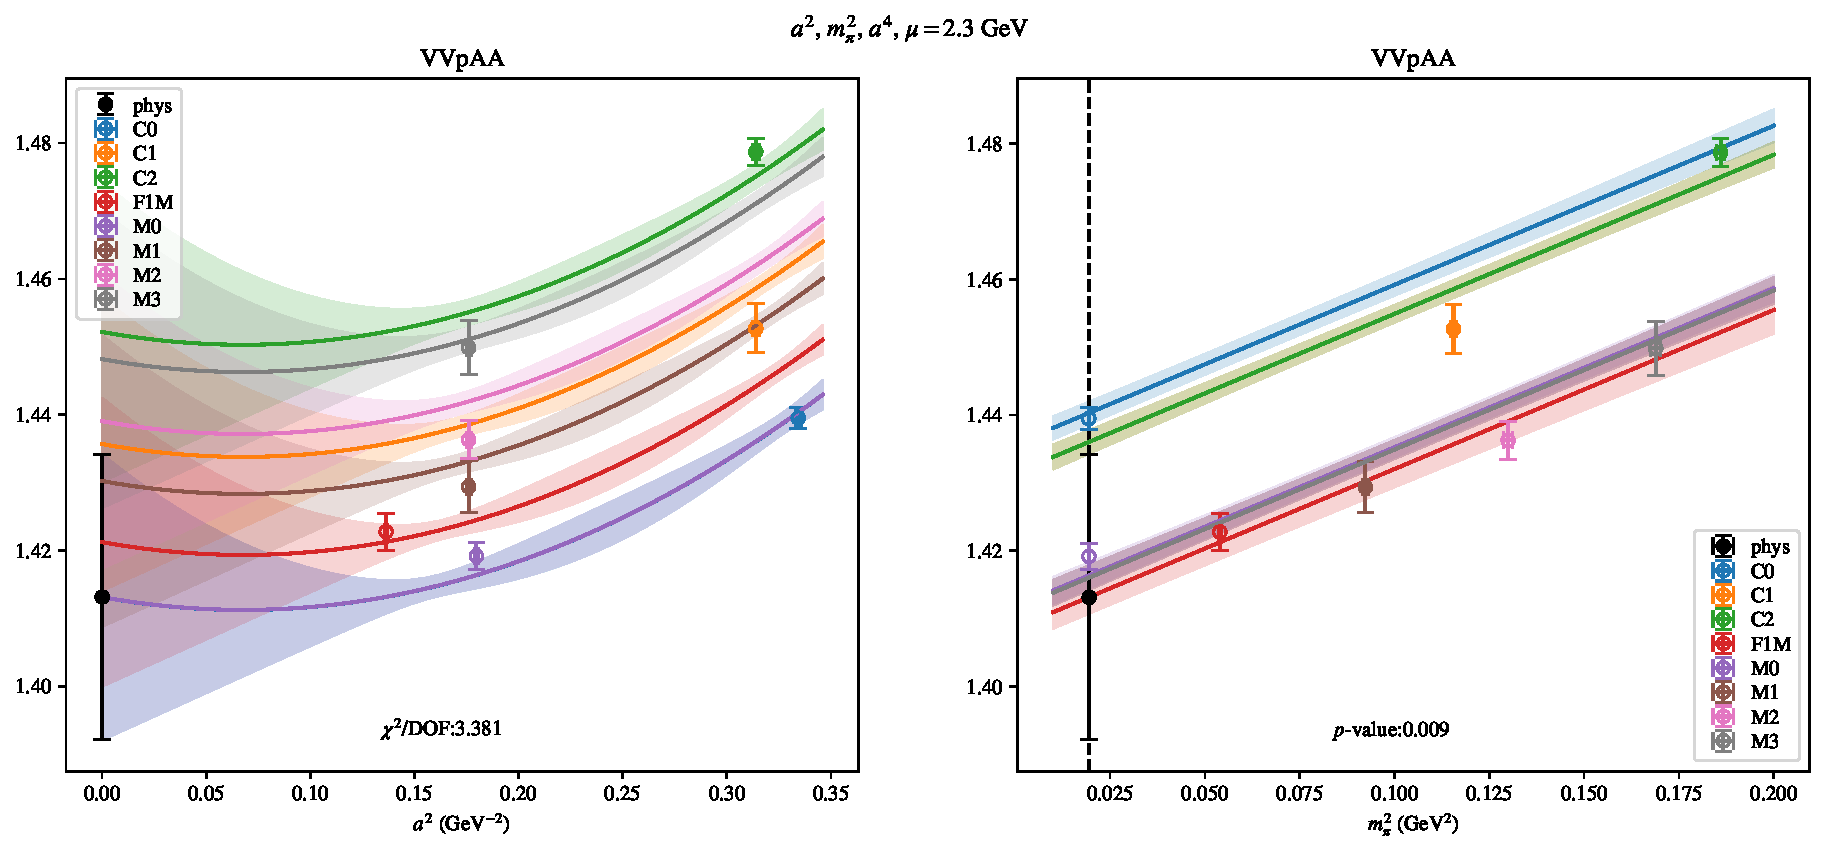
\includepdf[link, pages=-]{VVpAA/NPR/bag_a2a4m2_23.pdf}
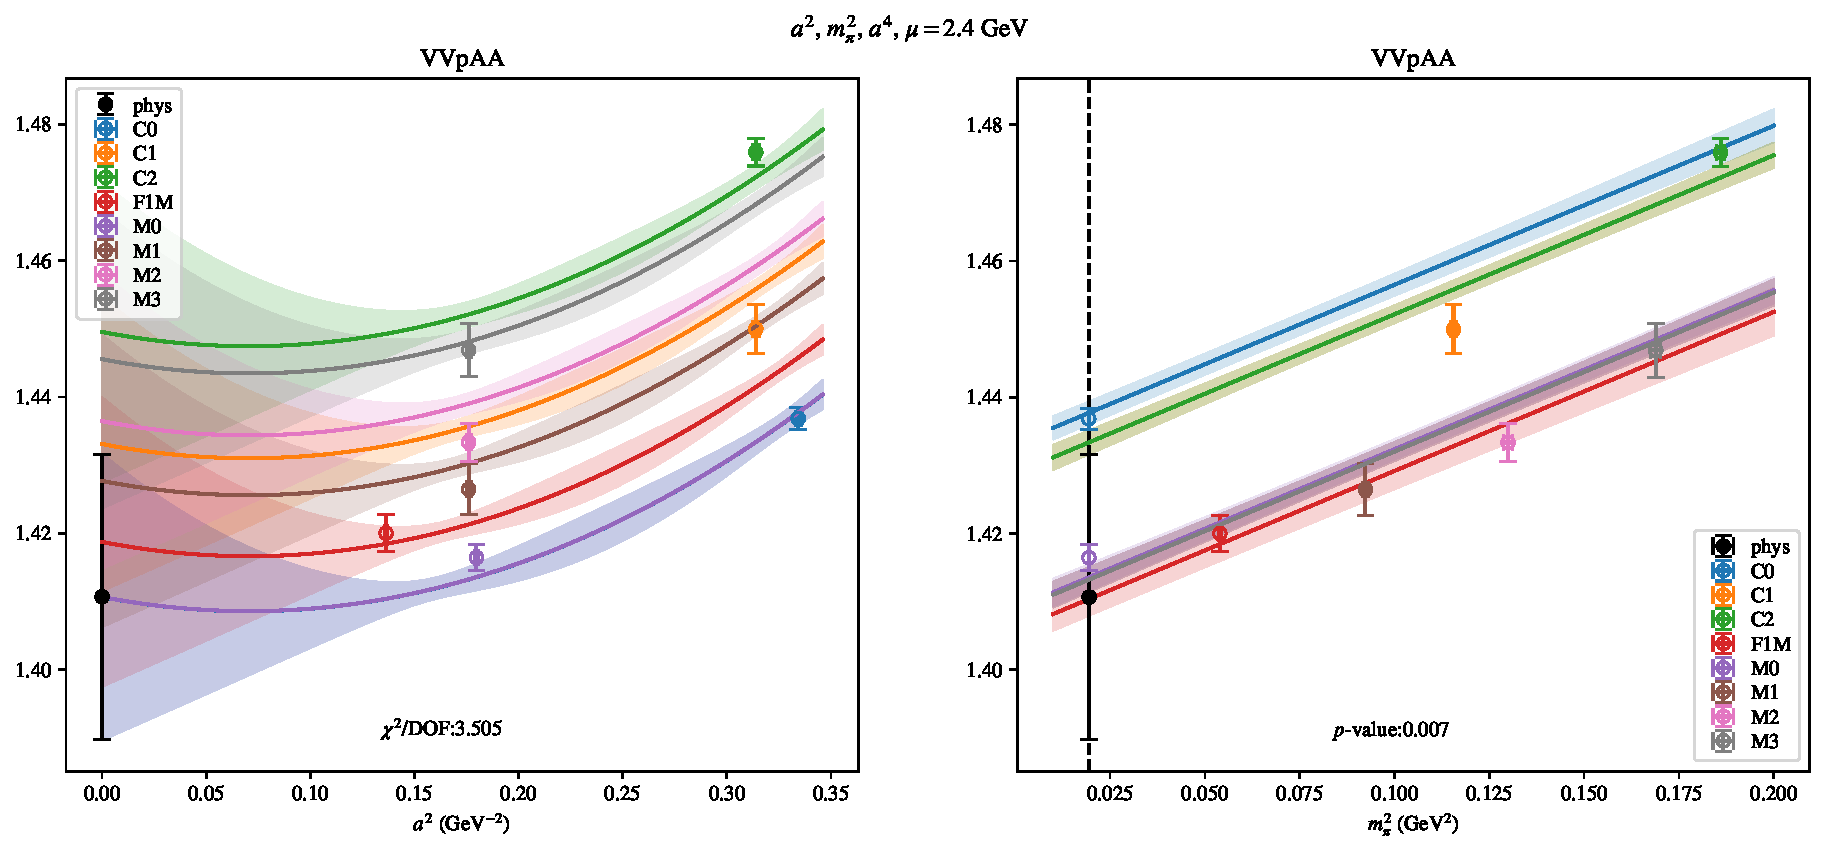
\includepdf[link, pages=-]{VVpAA/NPR/bag_a2a4m2_24.pdf}
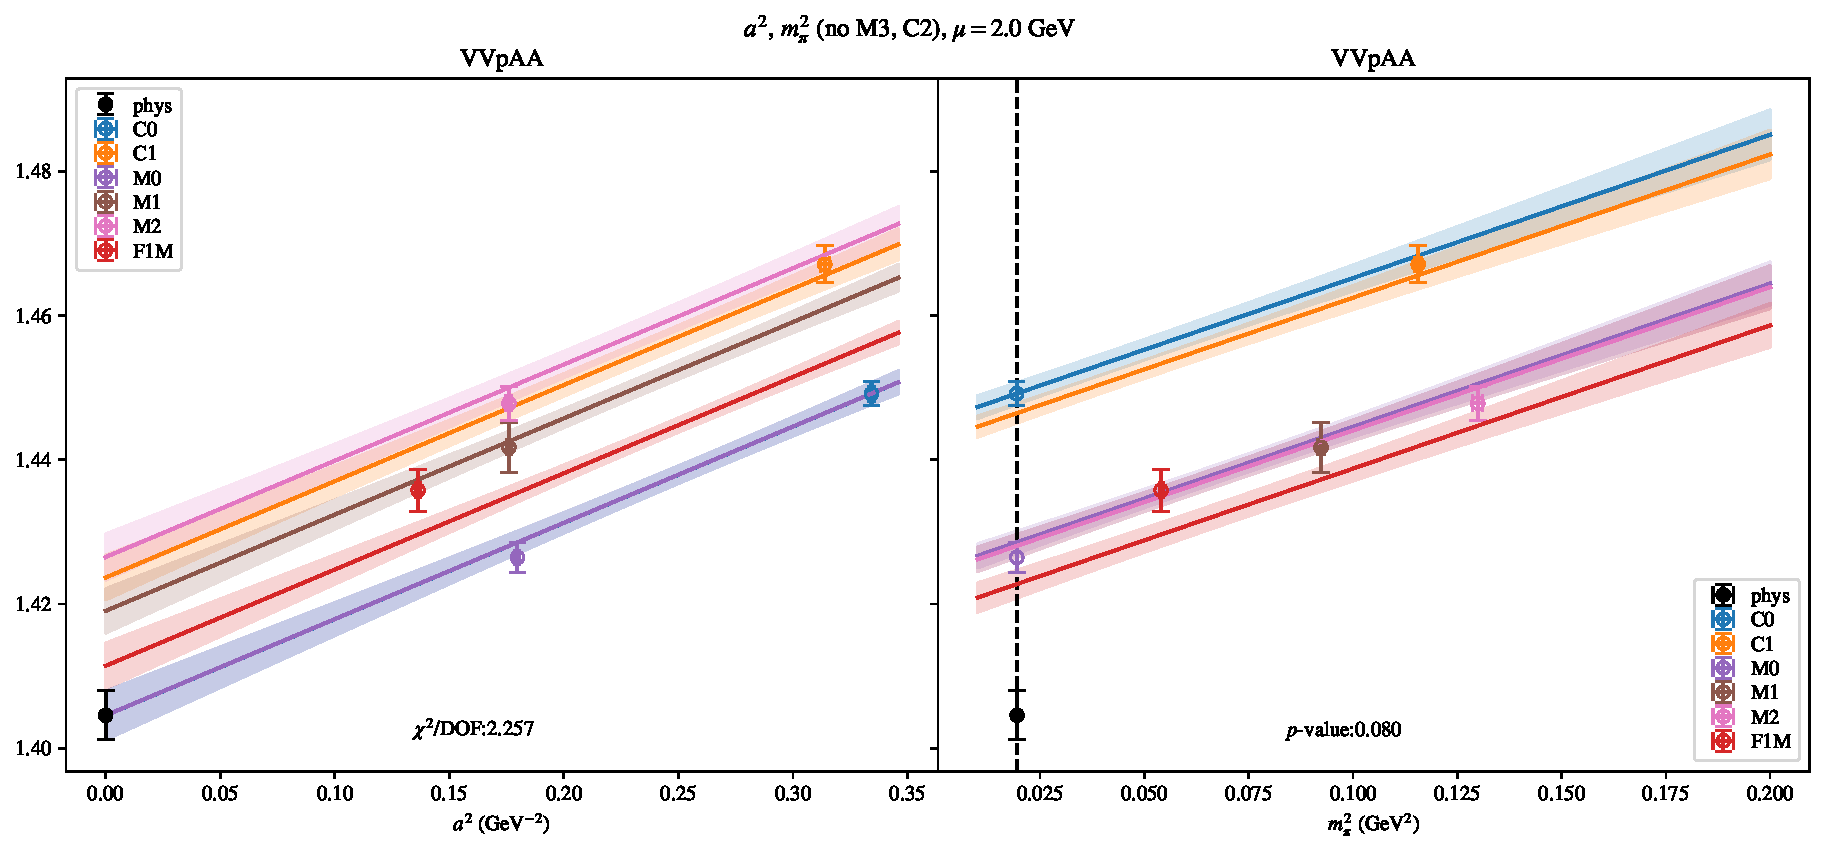
\includepdf[link, pages=-]{VVpAA/NPR/bag_a2m2mcut_20.pdf}
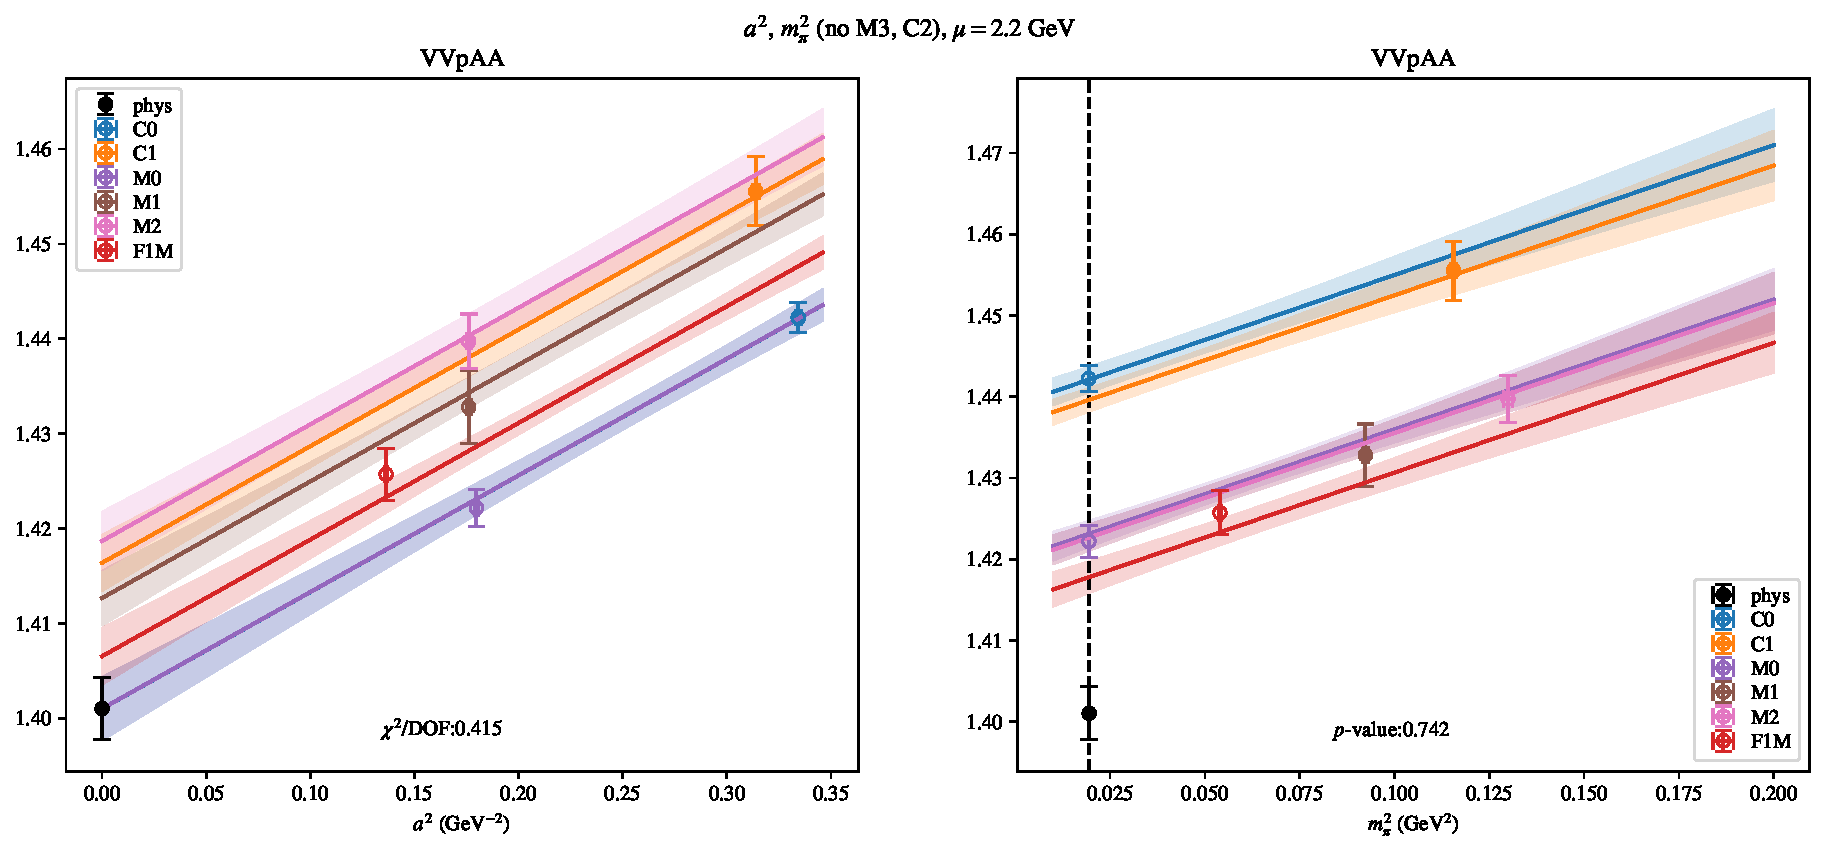
\includepdf[link, pages=-]{VVpAA/NPR/bag_a2m2mcut_22.pdf}
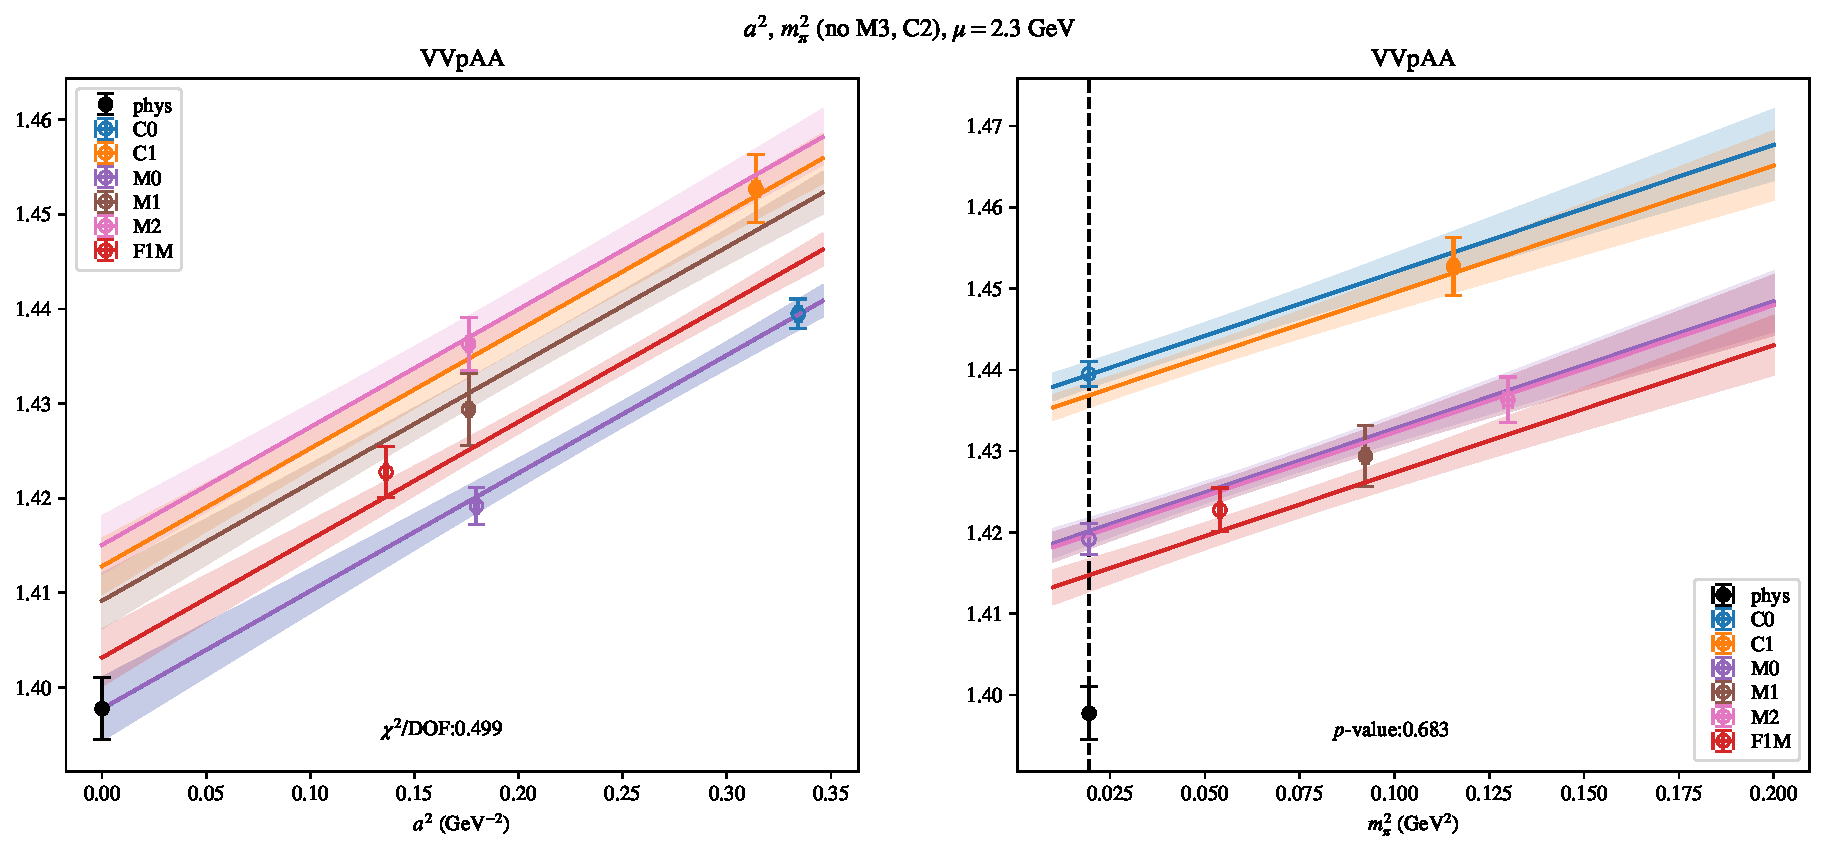
\includepdf[link, pages=-]{VVpAA/NPR/bag_a2m2mcut_23.pdf}
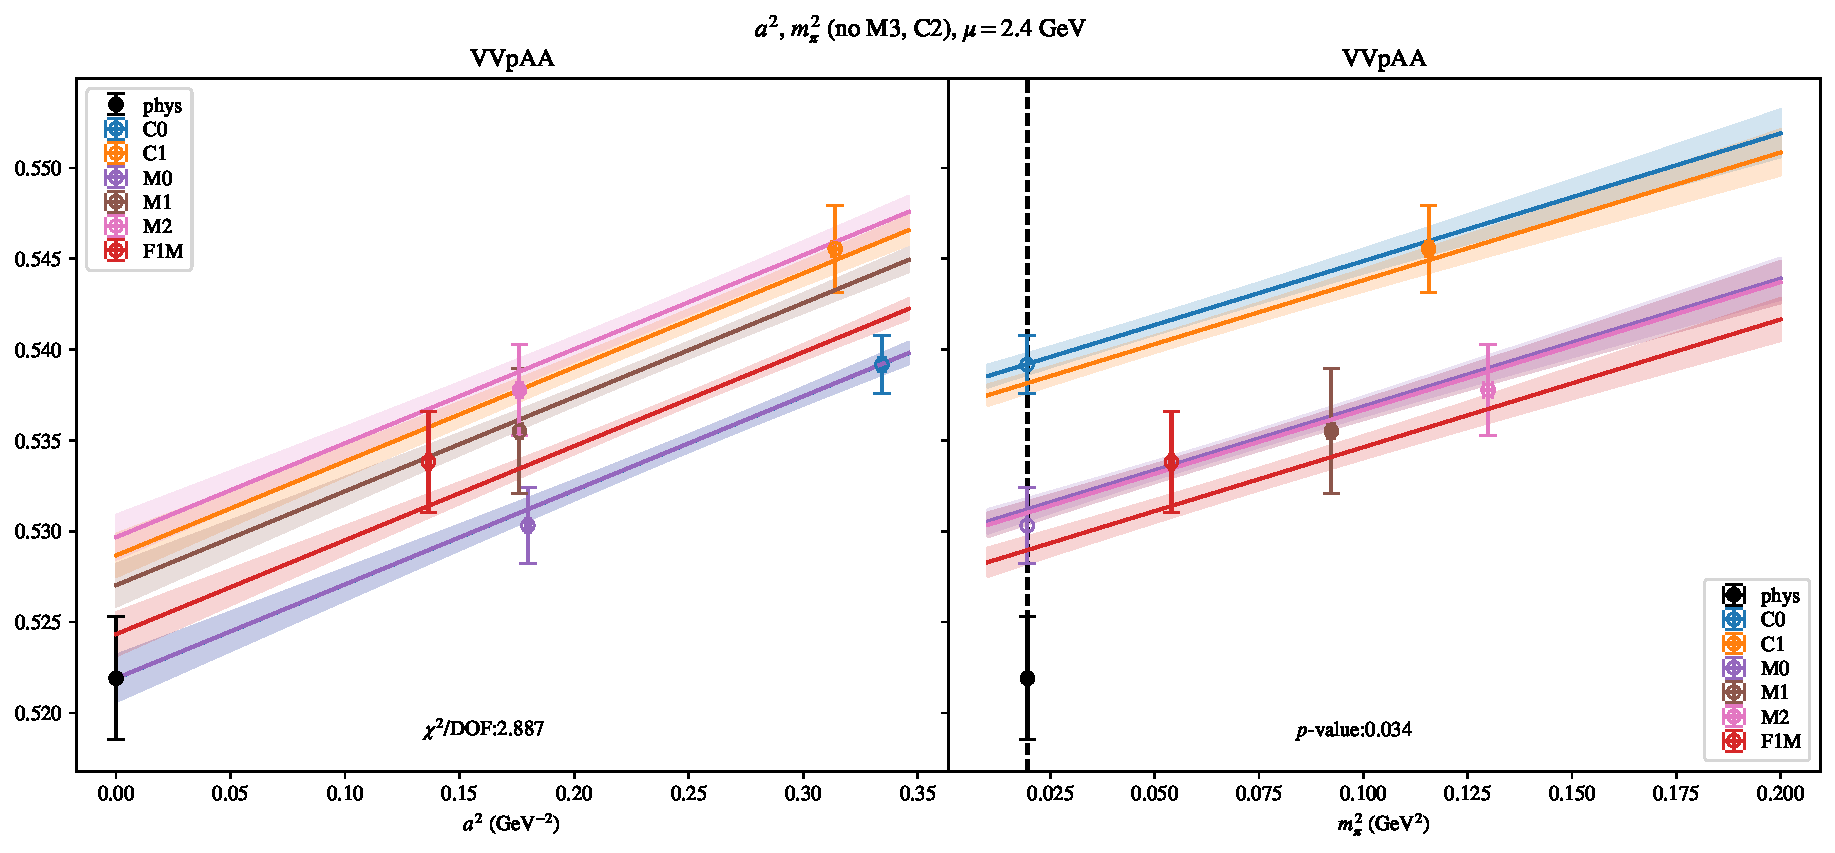
\includepdf[link, pages=-]{VVpAA/NPR/bag_a2m2mcut_24.pdf}
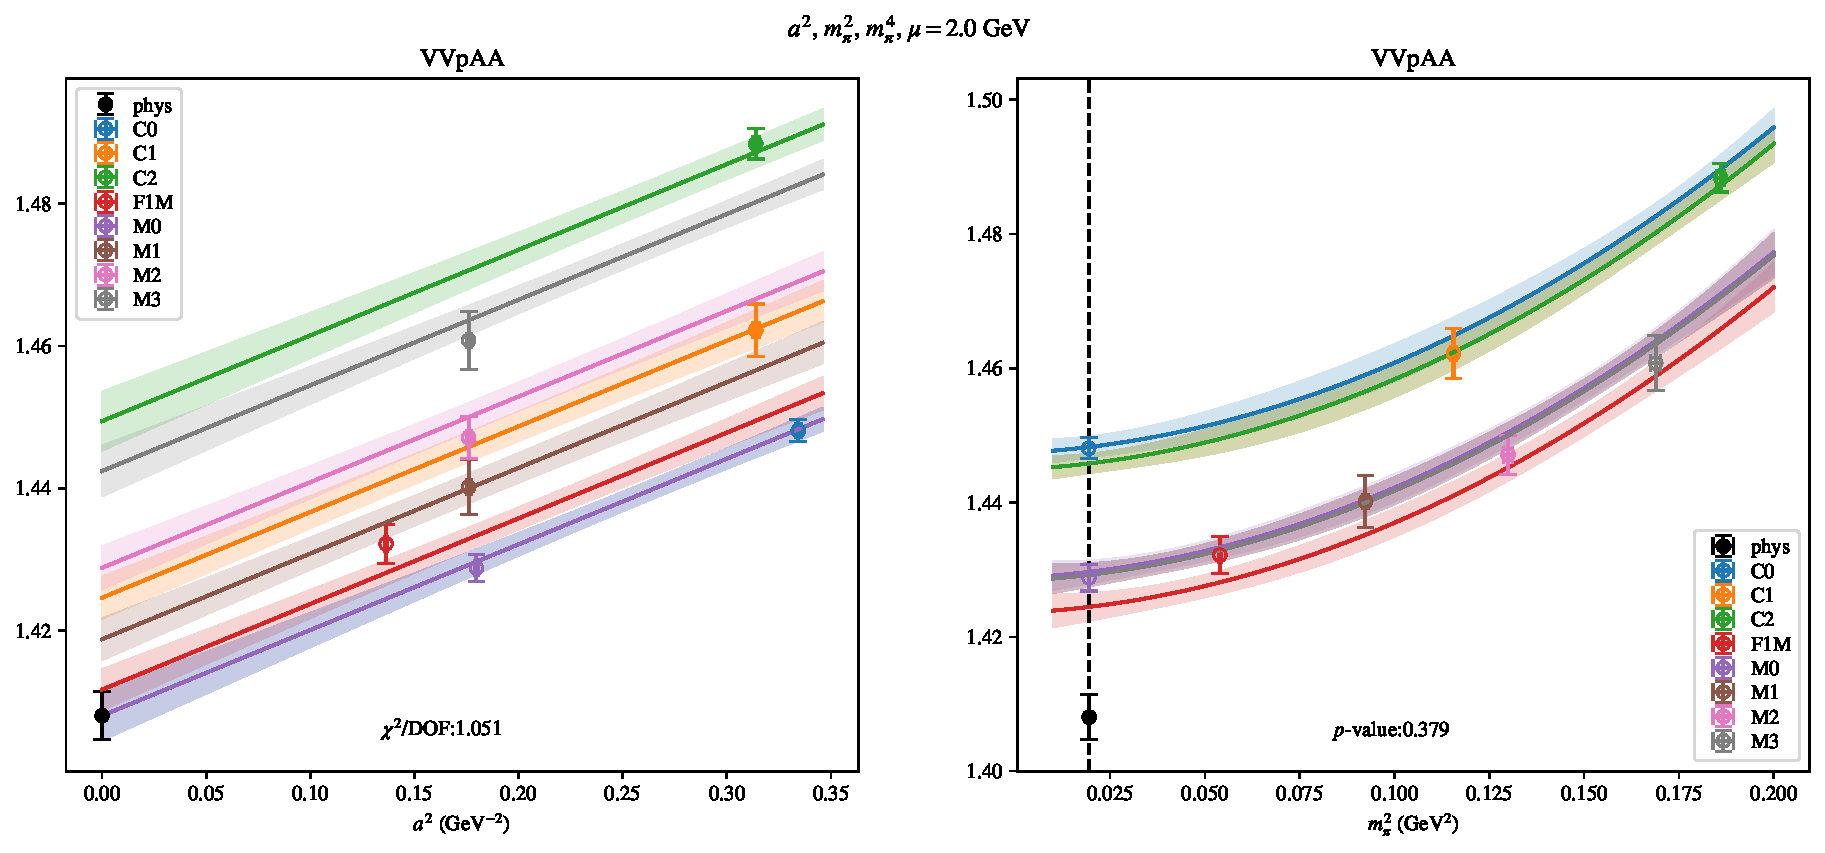
\includepdf[link, pages=-]{VVpAA/NPR/bag_a2m2m4_20.pdf}
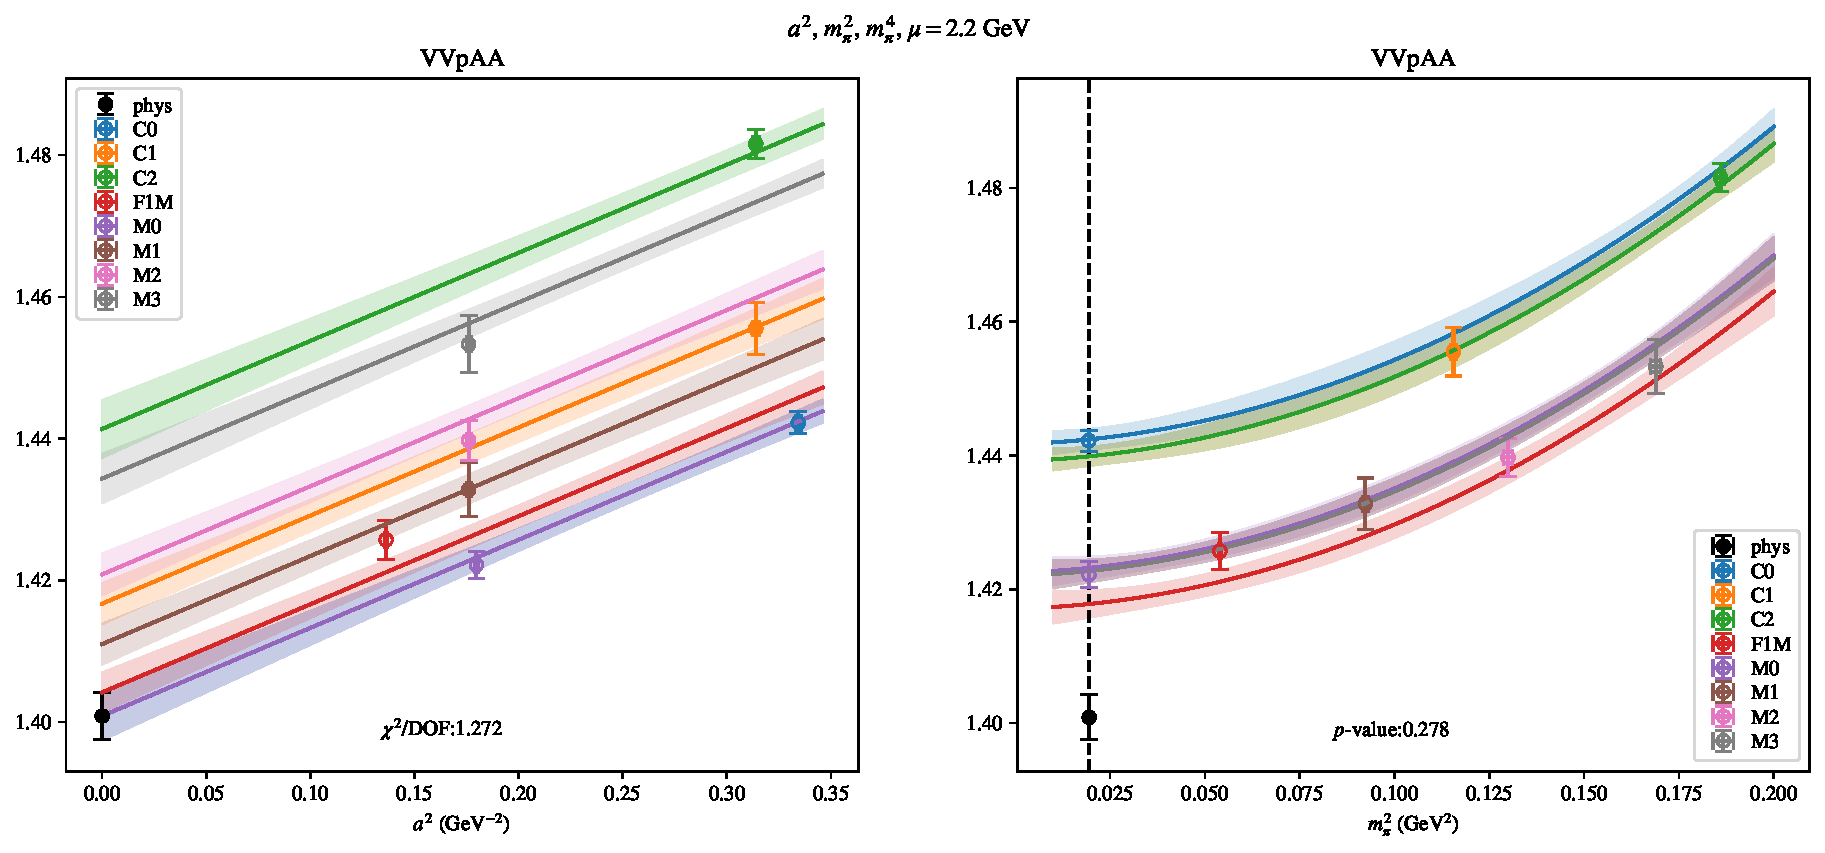
\includepdf[link, pages=-]{VVpAA/NPR/bag_a2m2m4_22.pdf}
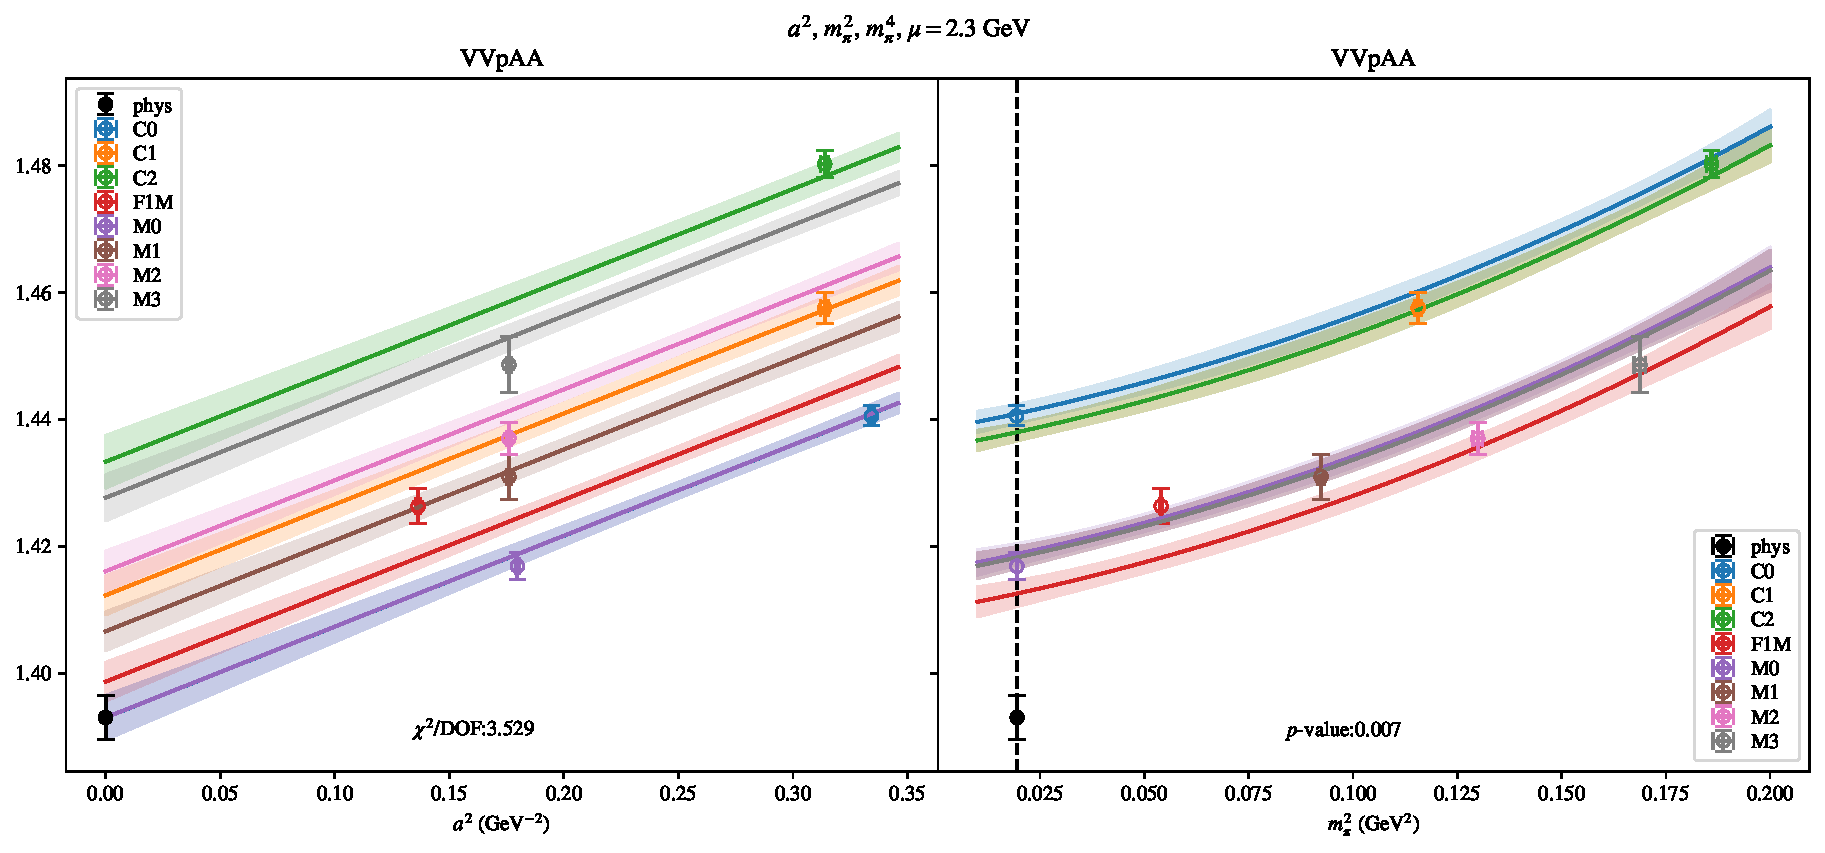
\includepdf[link, pages=-]{VVpAA/NPR/bag_a2m2m4_23.pdf}
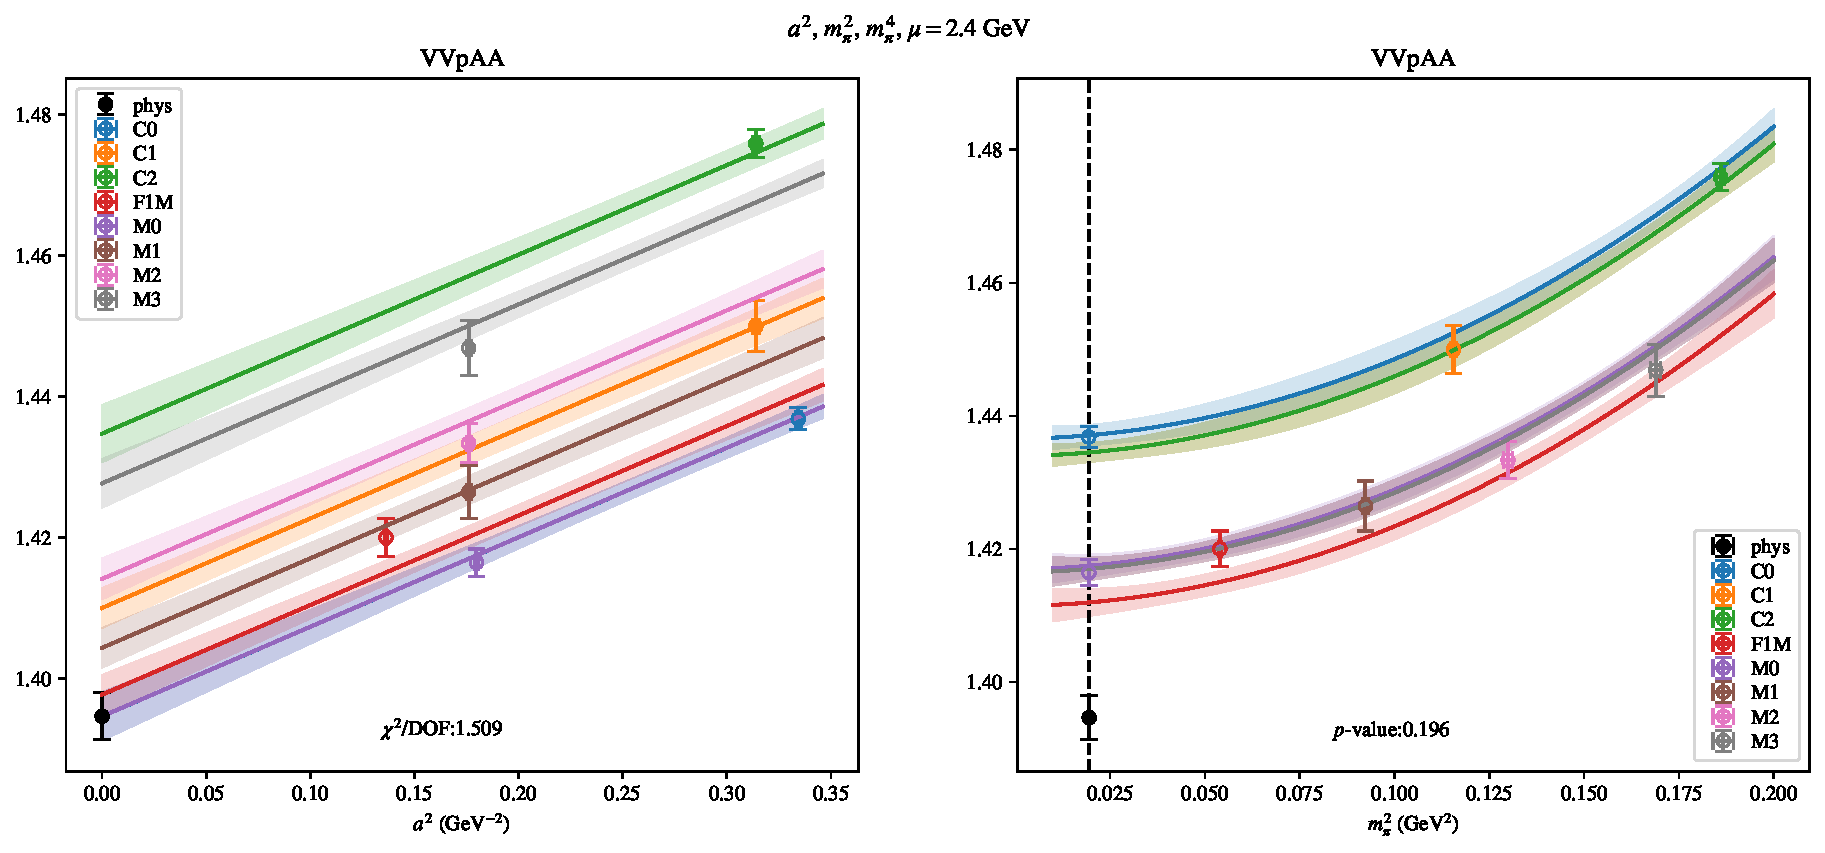
\includepdf[link, pages=-]{VVpAA/NPR/bag_a2m2m4_24.pdf}
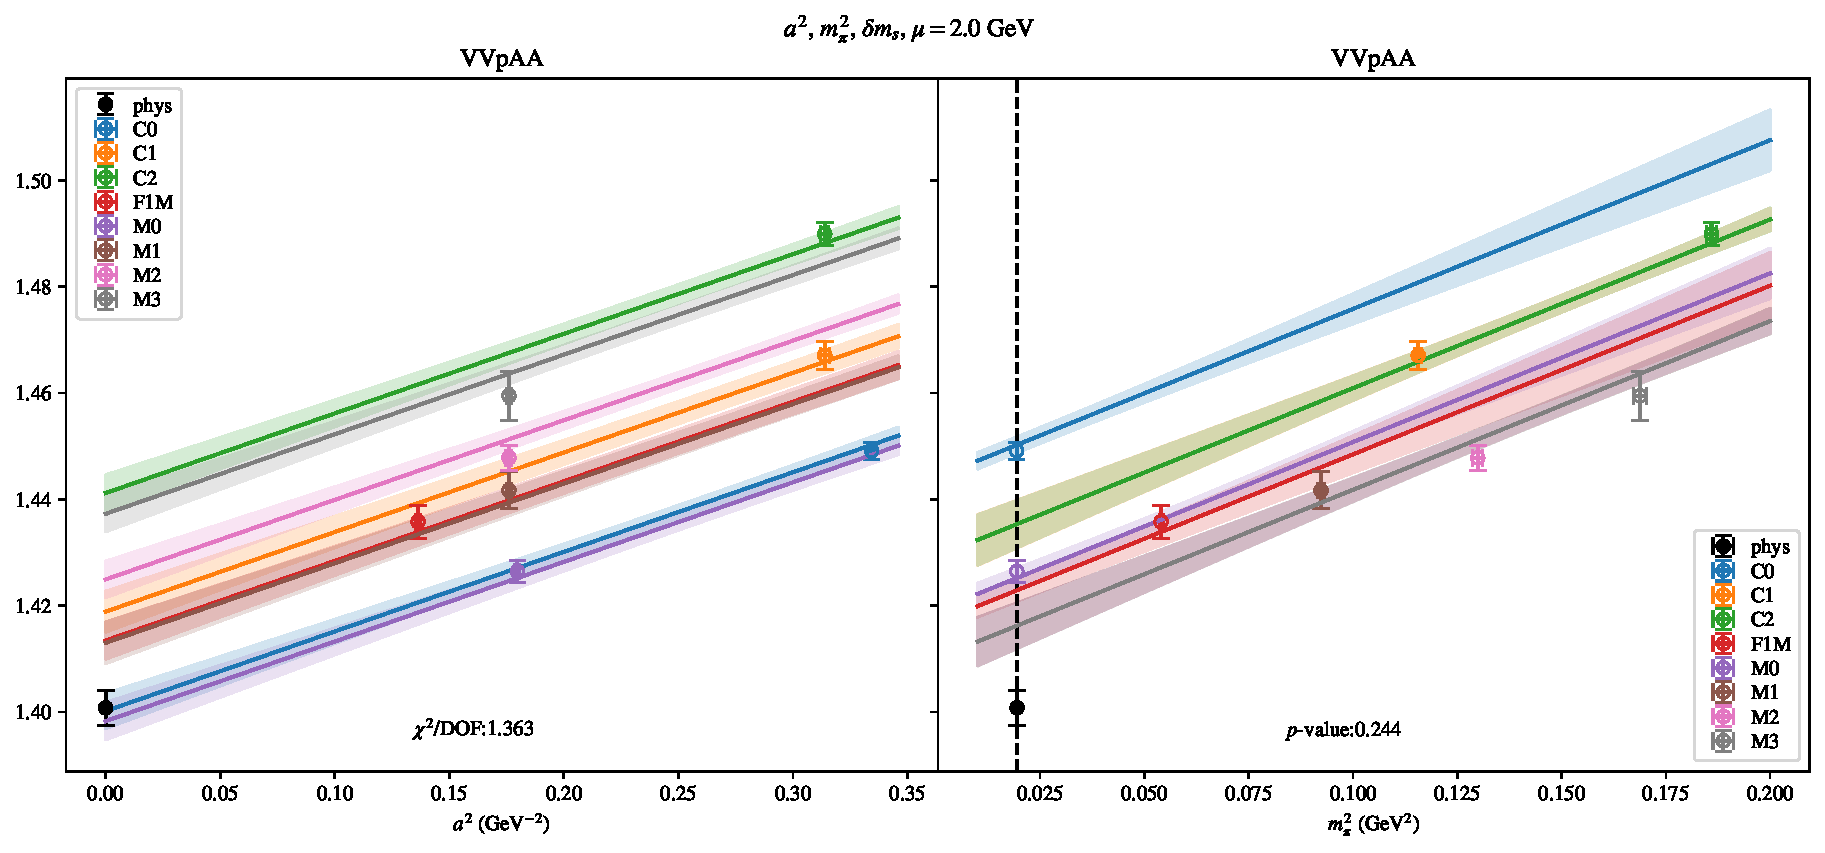
\includepdf[link, pages=-]{VVpAA/NPR/bag_a2m2delm_20.pdf}
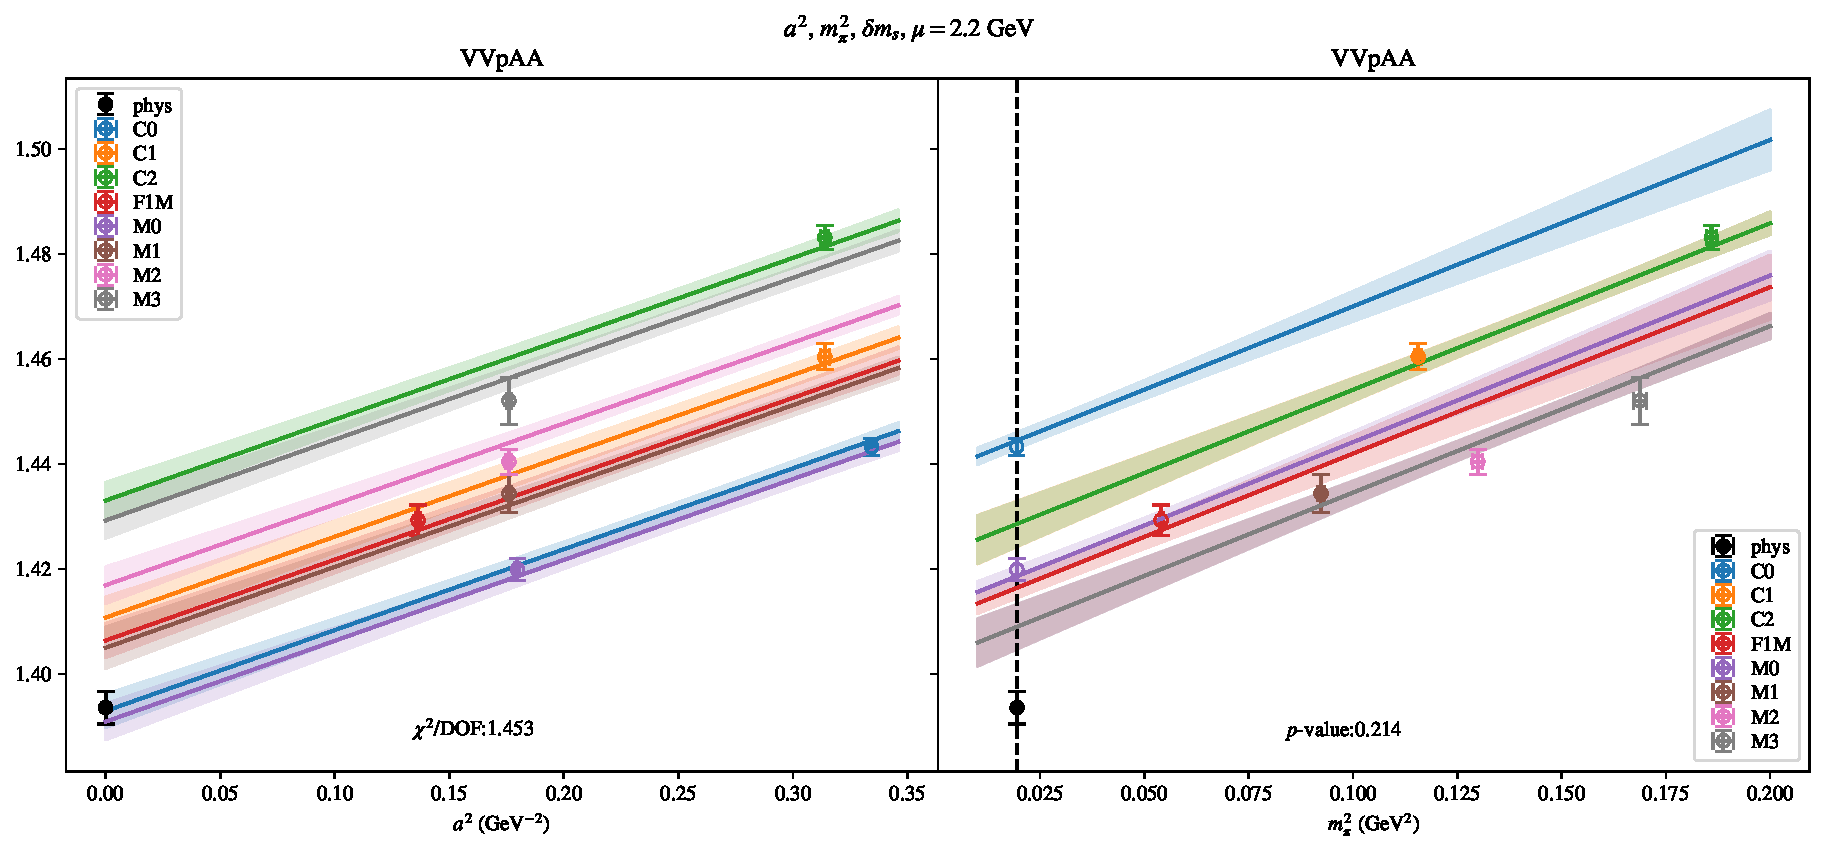
\includepdf[link, pages=-]{VVpAA/NPR/bag_a2m2delm_22.pdf}
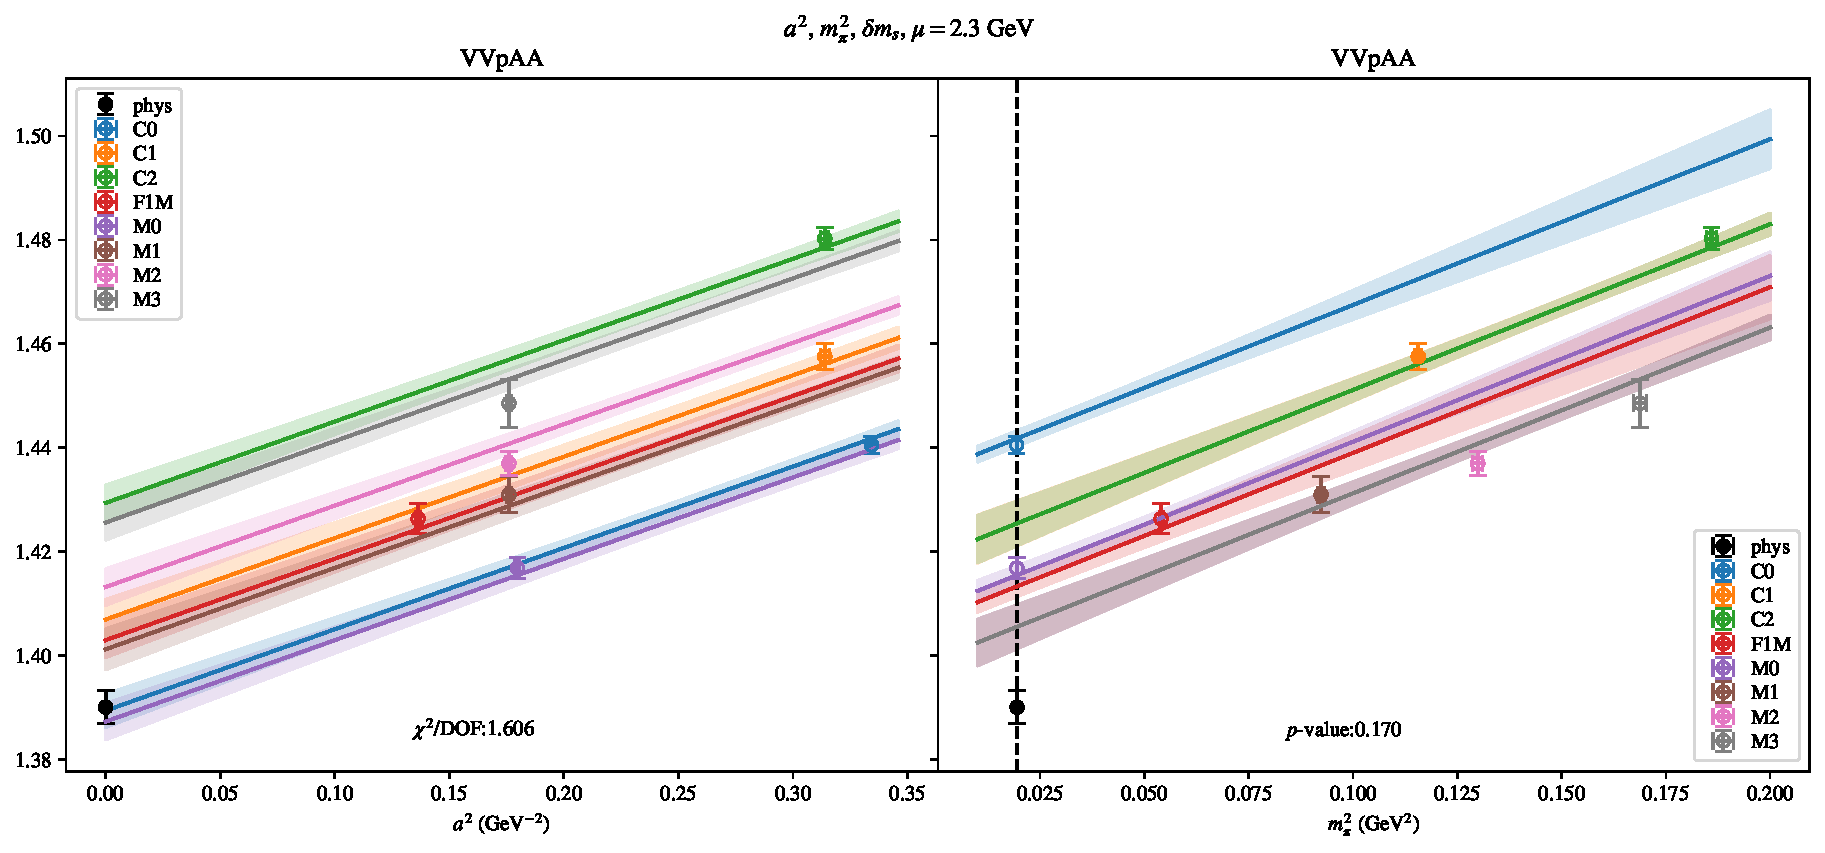
\includepdf[link, pages=-]{VVpAA/NPR/bag_a2m2delm_23.pdf}
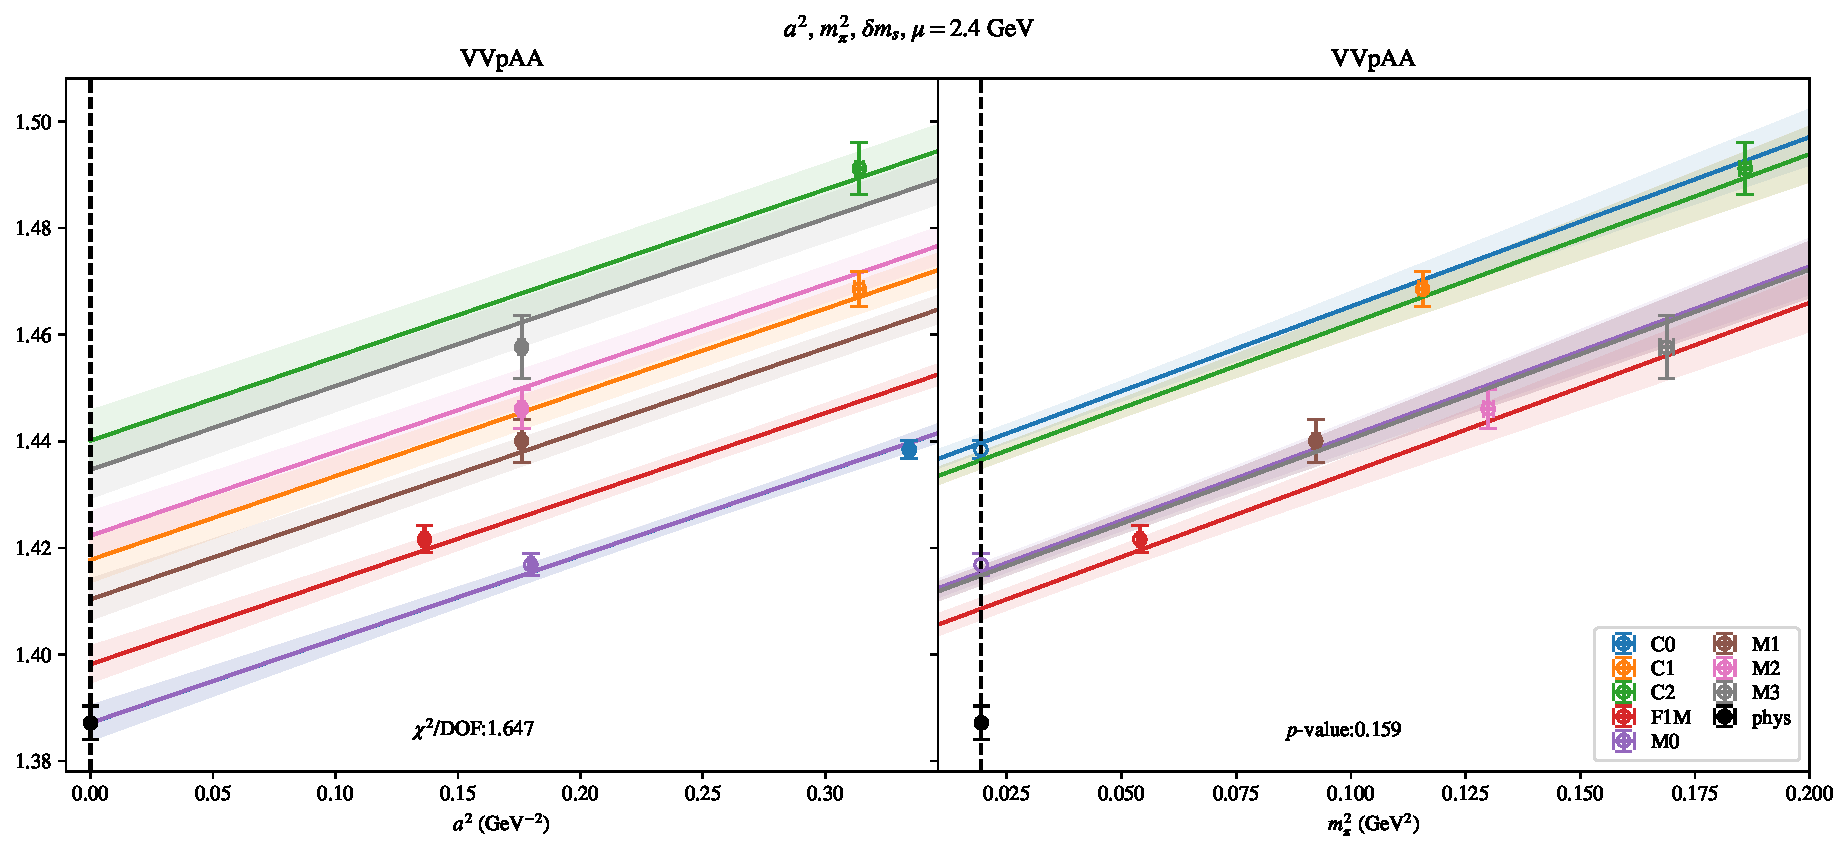
\includepdf[link, pages=-]{VVpAA/NPR/bag_a2m2delm_24.pdf}
\clearpage
\section{$\mathcal{B}_2$}
\begin{table}[h!]
\begin{center}
\begin{tabular}{|c|c|c|c|c|c|c|}
\hline
$\mu$ (GeV) & $a^2$, $m_\pi^2$& $a^2$, $m_\pi^2$ (no C)& $a^2$, $m_\pi^2$, $a^4$& $a^2$, $m_\pi^2$ (no M3, C2)& $a^2$, $m_\pi^2$, $m_\pi^4$& $a^2$, $m_\pi^2$, $\delta m_s$\\
\hline
2.0& \hyperlink{VVmAA/NPR/bag_a2m2_20.pdf.1}{\textbf{-0.987(15)}: 0.18 (0.97)} & \hyperlink{VVmAA/NPR/bag_a2m2noC_20.pdf.1}{\textbf{-0.935(60)}: 0.002 (0.998)} & \hyperlink{VVmAA/NPR/bag_a2a4m2_20.pdf.1}{\textbf{-0.905(86)}: 0.03 (0.998)} & \hyperlink{VVmAA/NPR/bag_a2m2mcut_20.pdf.1}{\textbf{-0.990(13)}: 0.291 (0.832)} & \hyperlink{VVmAA/NPR/bag_a2m2m4_20.pdf.1}{\textbf{-0.991(14)}: 0.174 (0.952)} & \hyperlink{VVmAA/NPR/bag_a2m2delm_20.pdf.1}{\textbf{-0.987(14)}: 0.085 (0.987)}\\
2.2& \hyperlink{VVmAA/NPR/bag_a2m2_22.pdf.1}{\textbf{-1.001(12)}: 0.231 (0.949)} & \hyperlink{VVmAA/NPR/bag_a2m2noC_22.pdf.1}{\textbf{-0.959(51)}: 0.009 (0.991)} & \hyperlink{VVmAA/NPR/bag_a2a4m2_22.pdf.1}{\textbf{-0.930(68)}: 0.024 (0.999)} & \hyperlink{VVmAA/NPR/bag_a2m2mcut_22.pdf.1}{\textbf{-1.000(12)}: 0.347 (0.791)} & \hyperlink{VVmAA/NPR/bag_a2m2m4_22.pdf.1}{\textbf{-1.004(13)}: 0.176 (0.951)} & \hyperlink{VVmAA/NPR/bag_a2m2delm_22.pdf.1}{\textbf{-1.001(12)}: 0.115 (0.977)}\\
2.3& \hyperlink{VVmAA/NPR/bag_a2m2_23.pdf.1}{\textbf{-1.008(12)}: 0.237 (0.946)} & \hyperlink{VVmAA/NPR/bag_a2m2noC_23.pdf.1}{\textbf{-0.966(44)}: 0.008 (0.992)} & \hyperlink{VVmAA/NPR/bag_a2a4m2_23.pdf.1}{\textbf{-0.938(68)}: 0.02 (0.999)} & \hyperlink{VVmAA/NPR/bag_a2m2mcut_23.pdf.1}{\textbf{-1.008(10)}: 0.389 (0.761)} & \hyperlink{VVmAA/NPR/bag_a2m2m4_23.pdf.1}{\textbf{-1.010(11)}: 0.235 (0.919)} & \hyperlink{VVmAA/NPR/bag_a2m2delm_23.pdf.1}{\textbf{-1.007(11)}: 0.128 (0.972)}\\
2.4& \hyperlink{VVmAA/NPR/bag_a2m2_24.pdf.1}{\textbf{-1.012(10)}: 0.256 (0.937)} & \hyperlink{VVmAA/NPR/bag_a2m2noC_24.pdf.1}{\textbf{-0.974(39)}: 0.01 (0.99)} & \hyperlink{VVmAA/NPR/bag_a2a4m2_24.pdf.1}{\textbf{-0.946(61)}: 0.022 (0.999)} & \hyperlink{VVmAA/NPR/bag_a2m2mcut_24.pdf.1}{\textbf{-1.0114(93)}: 0.413 (0.743)} & \hyperlink{VVmAA/NPR/bag_a2m2m4_24.pdf.1}{\textbf{-1.015(10)}: 0.242 (0.915)} & \hyperlink{VVmAA/NPR/bag_a2m2delm_24.pdf.1}{\textbf{-1.012(10)}: 0.134 (0.97)}\\
\hline
\end{tabular}
\caption{Physical point value from chiral and continuum extrapolation at renormalisation scale $\mu$. Entries are \textbf{value(error)}: $\chi^2/\text{DOF}$ ($p$-value).}
\end{center}
\end{table}
\begin{table}[h!]
\begin{center}
\begin{tabular}{|c c|c|c|c|c|c|c|}
\hline
$\mu$ (GeV) &  & $a^2$, $m_\pi^2$& $a^2$, $m_\pi^2$ (no C)& $a^2$, $m_\pi^2$, $a^4$& $a^2$, $m_\pi^2$ (no M3, C2)& $a^2$, $m_\pi^2$, $m_\pi^4$& $a^2$, $m_\pi^2$, $\delta m_s$\\
\hline
\multirow{3}{0.5in}{2.0} & $\alpha$ & 0.168(55)& -0.14(35)& -0.59(79)& 0.177(46)& 0.178(50)& 0.172(54)\\
 & $\beta$ & -0.0020(15)& -0.0023(30)& -0.0018(15)& -0.0017(22)& 0.0014(41)& -0.0002(23)\\
 & $\gamma$ &  &  & 1.5(16)&  & -0.00031(32)& -0.071(97)\\
\hline
\multirow{3}{0.5in}{2.2} & $\alpha$ & 0.211(41)& -0.04(30)& -0.44(64)& 0.210(41)& 0.221(47)& 0.215(43)\\
 & $\beta$ & -0.0017(12)& -0.0016(24)& -0.0014(11)& -0.0013(16)& 0.0011(35)& -0.0002(19)\\
 & $\gamma$ &  &  & 1.3(13)&  & -0.00026(26)& -0.058(77)\\
\hline
\multirow{3}{0.5in}{2.3} & $\alpha$ & 0.237(43)& -0.01(26)& -0.40(63)& 0.238(36)& 0.242(39)& 0.237(40)\\
 & $\beta$ & -0.0018(11)& -0.0017(21)& -0.00151(99)& -0.0014(15)& 0.0014(33)& -0.0004(17)\\
 & $\gamma$ &  &  & 1.3(12)&  & -0.00029(24)& -0.052(69)\\
\hline
\multirow{3}{0.5in}{2.4} & $\alpha$ & 0.256(37)& 0.03(23)& -0.35(58)& 0.254(33)& 0.264(35)& 0.258(39)\\
 & $\beta$ & -0.0018(10)& -0.0016(18)& -0.00150(99)& -0.0015(14)& 0.0011(29)& -0.0004(15)\\
 & $\gamma$ &  &  & 1.2(12)&  & -0.00027(21)& -0.052(63)\\
\hline
\end{tabular}
\caption{Fit values of coefficients in $Q = Q_{phys} + \mathbf{\alpha} a^2 + \mathbf{\beta}\left(\frac{m_\pi^2}{f_\pi^2}-\frac{m_{\pi,PDG}^2}{f_\pi^2}\right) + \gamma(\ldots)$}
\end{center}
\end{table}
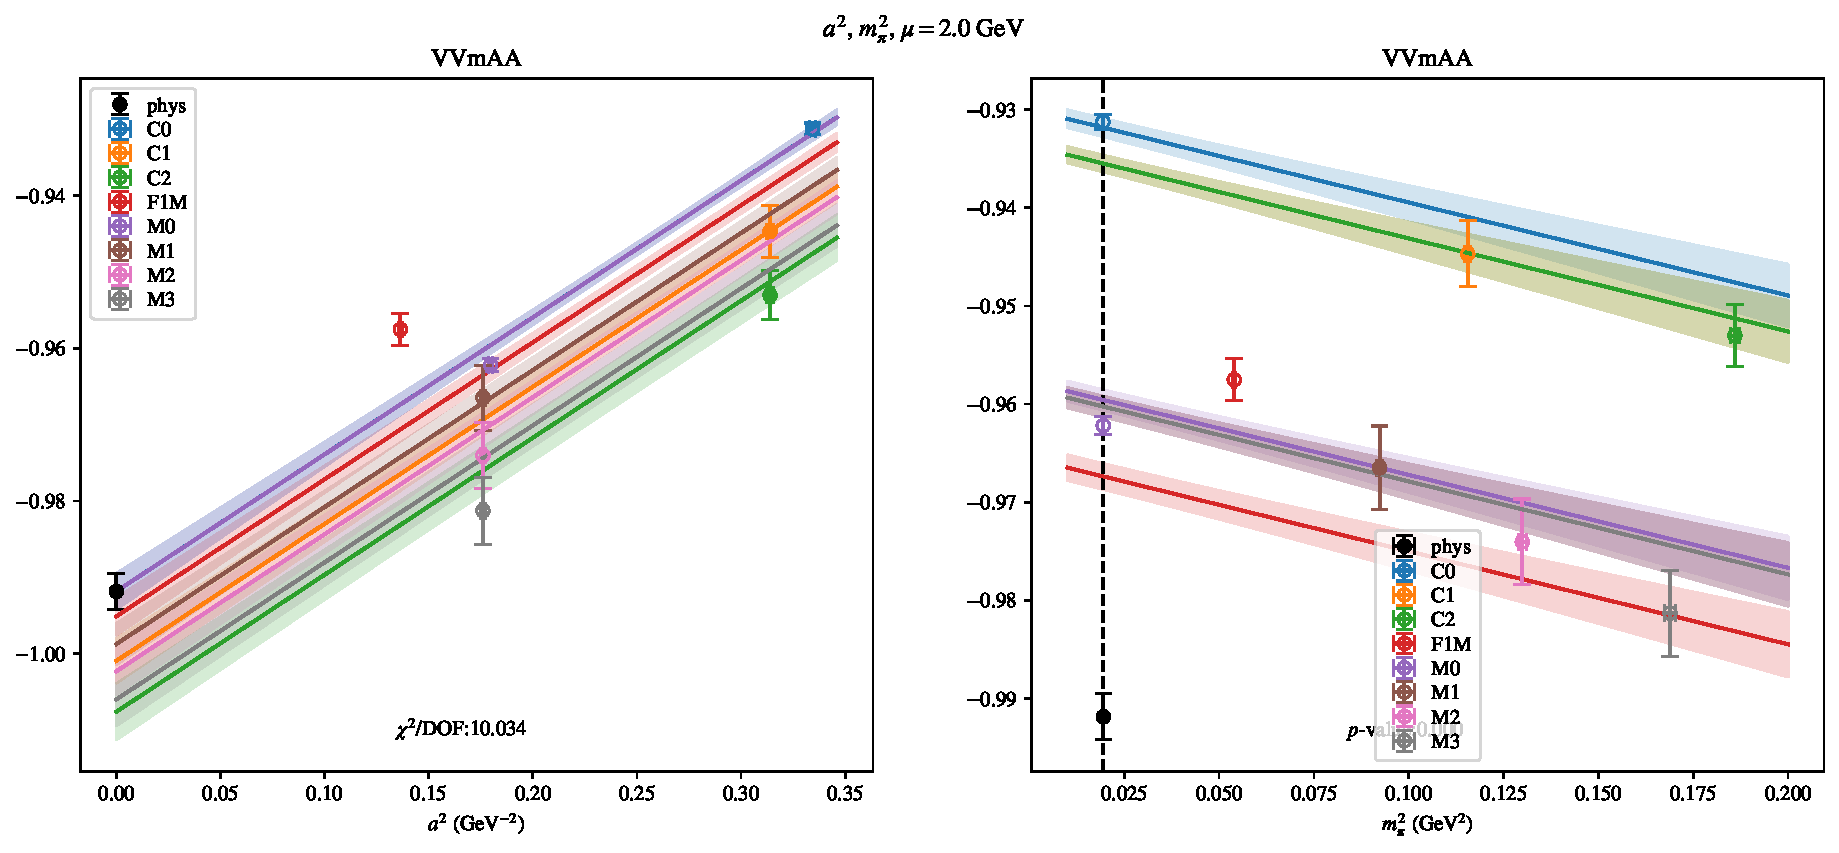
\includepdf[link, pages=-]{VVmAA/NPR/bag_a2m2_20.pdf}
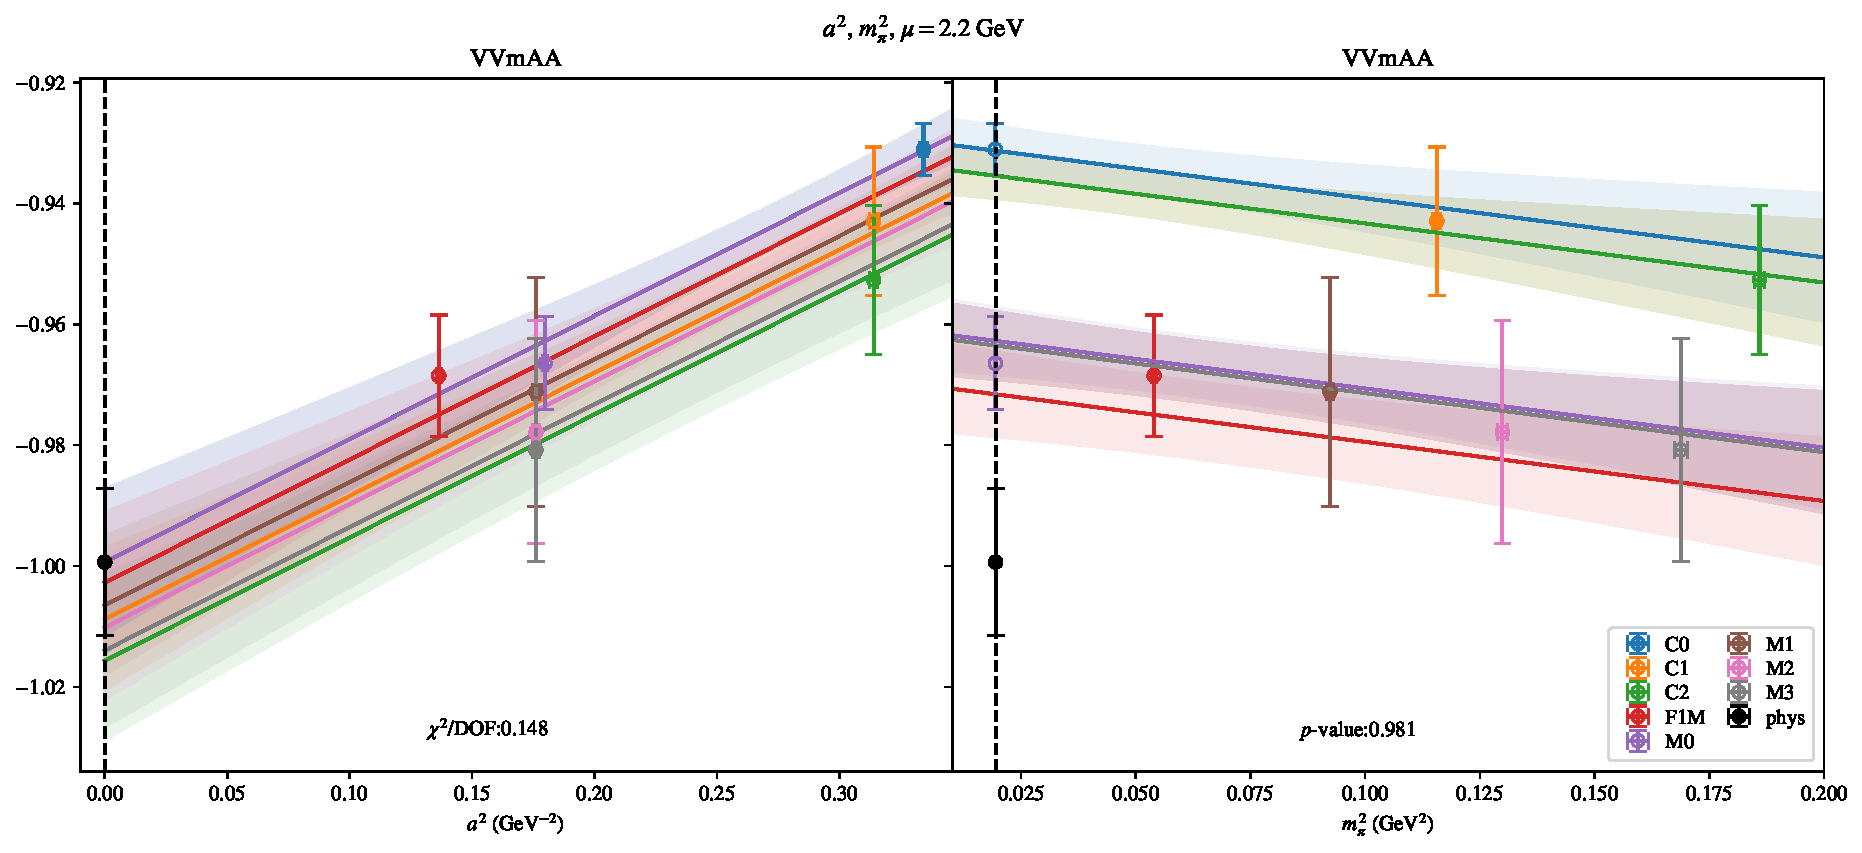
\includepdf[link, pages=-]{VVmAA/NPR/bag_a2m2_22.pdf}
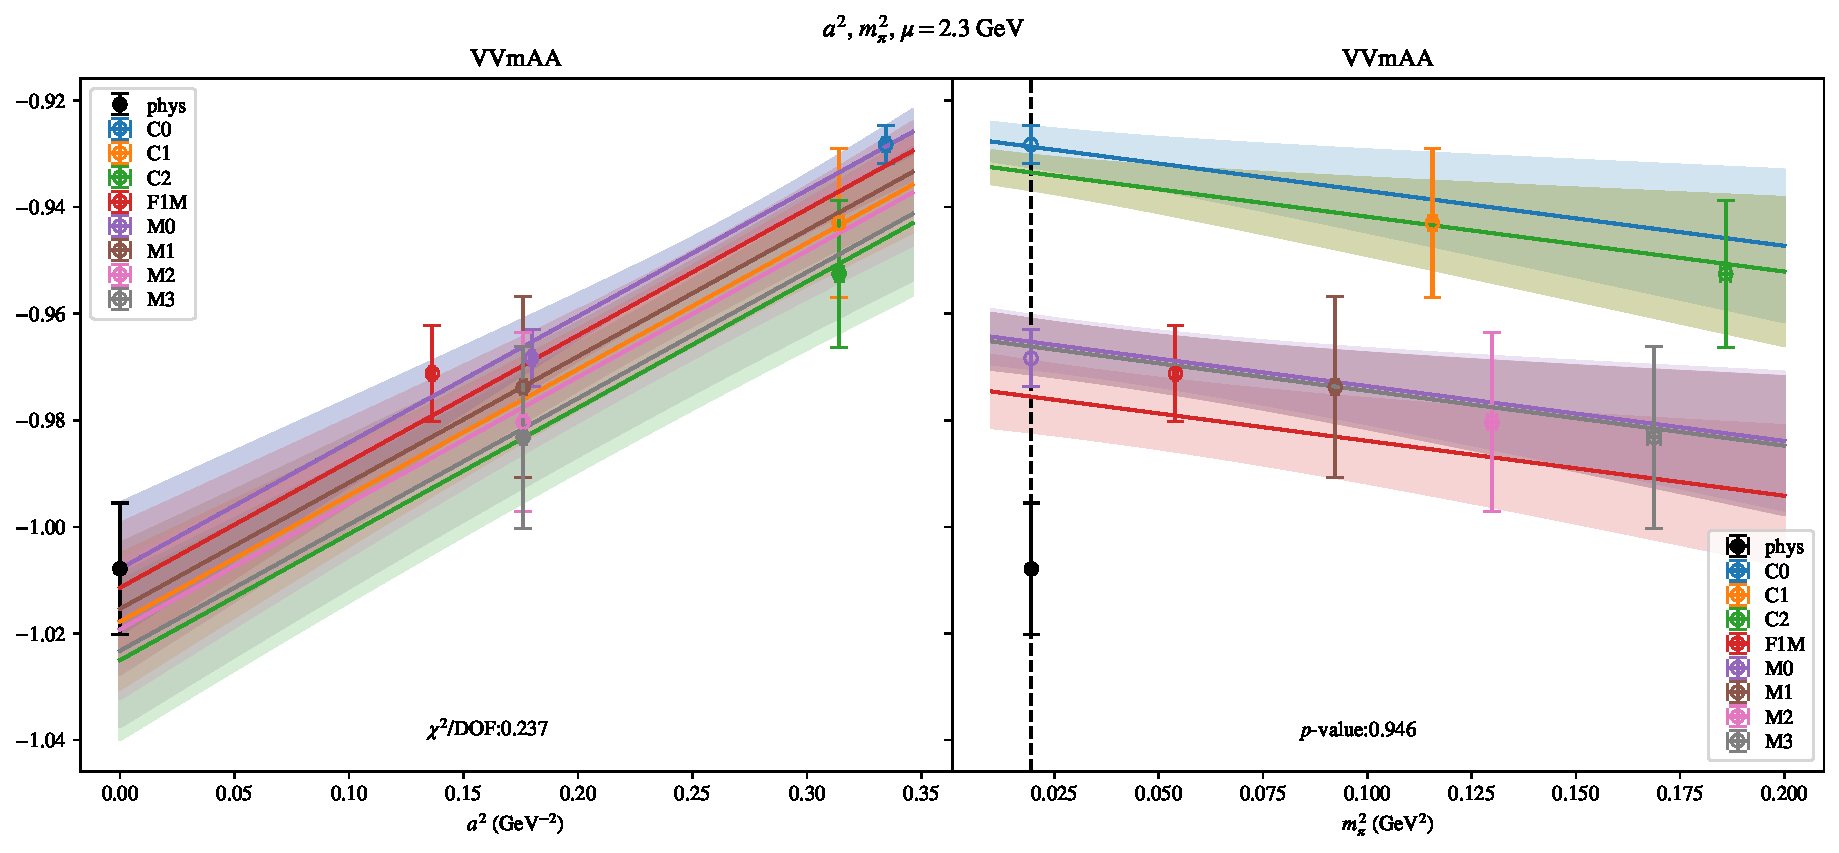
\includepdf[link, pages=-]{VVmAA/NPR/bag_a2m2_23.pdf}
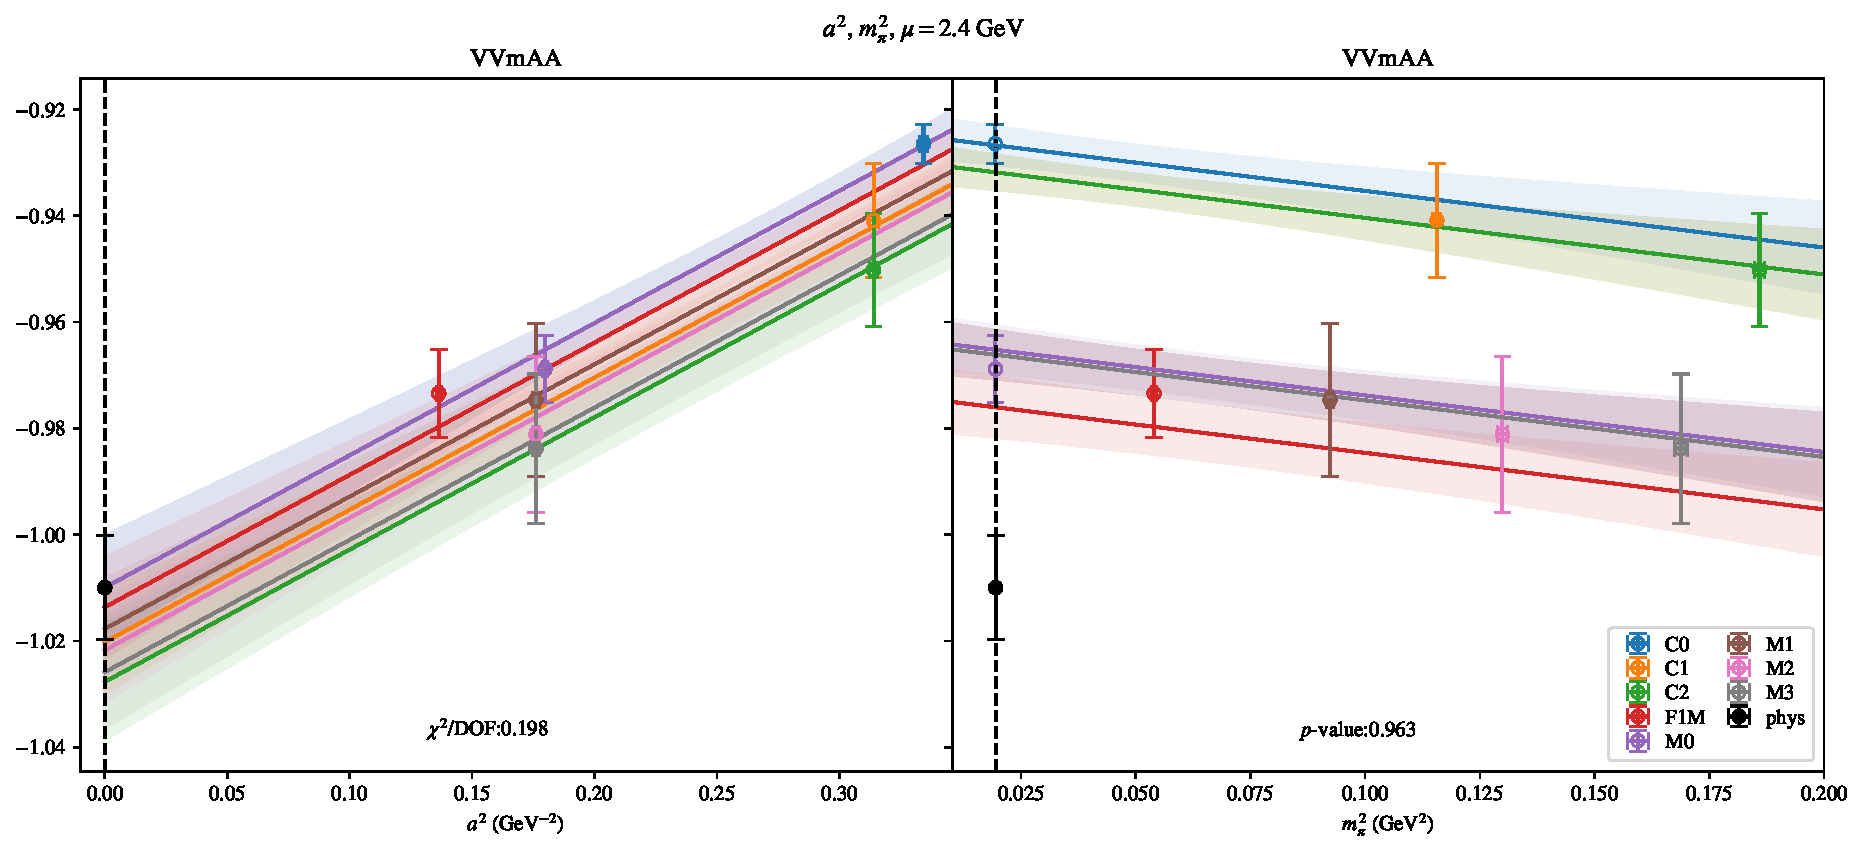
\includepdf[link, pages=-]{VVmAA/NPR/bag_a2m2_24.pdf}
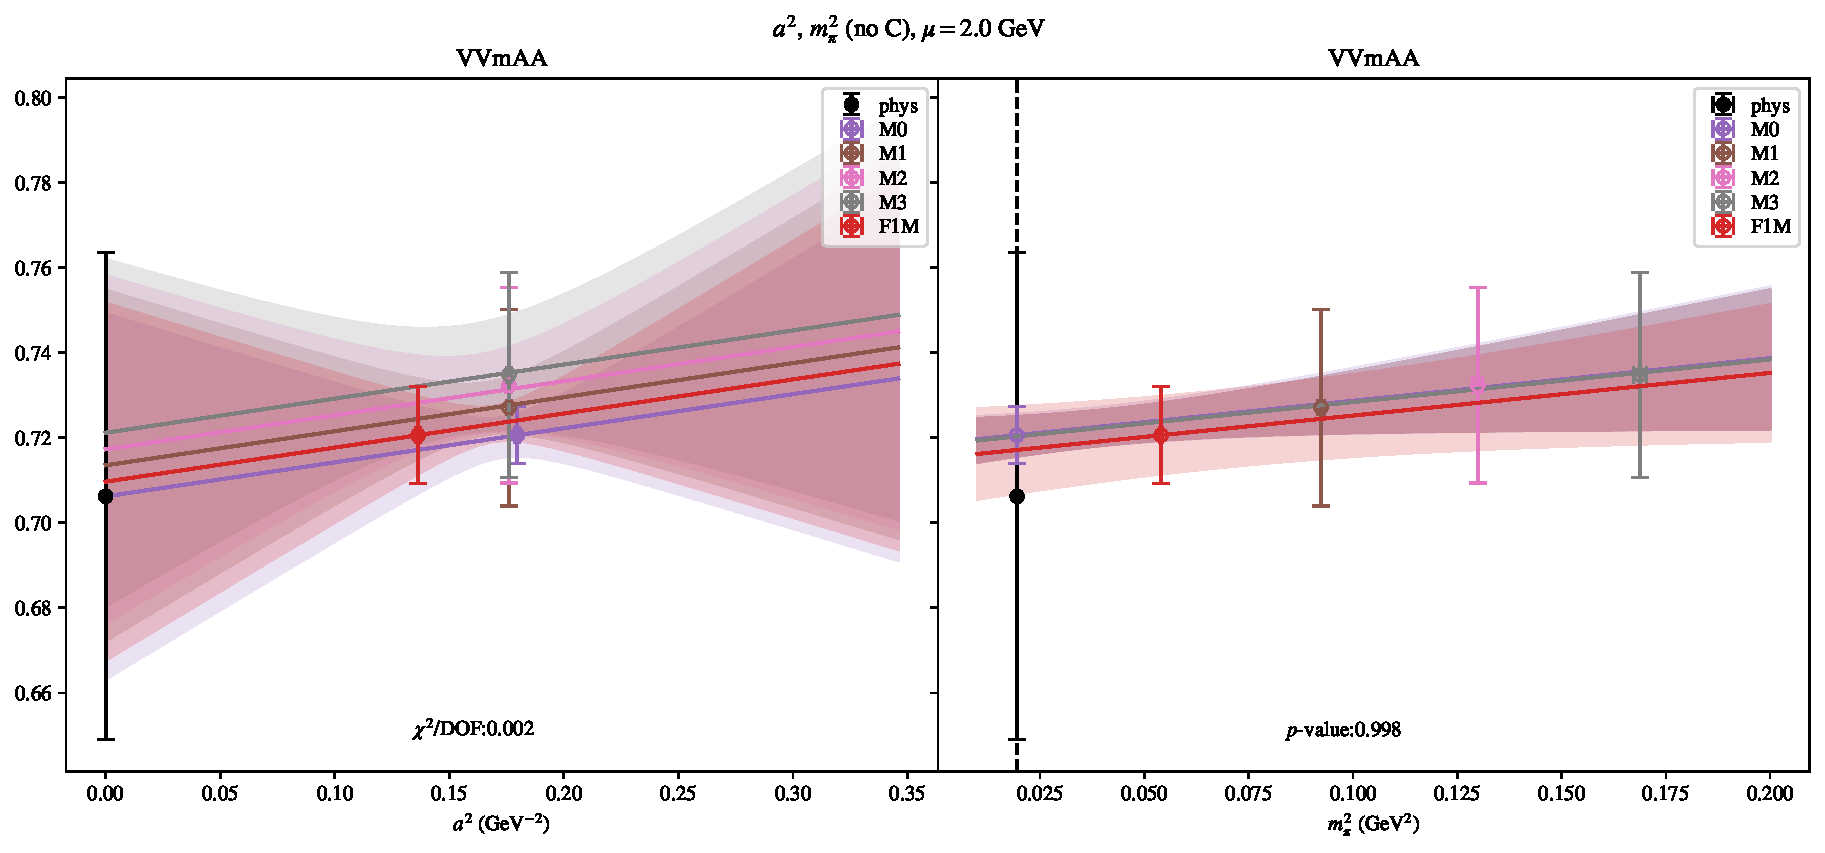
\includepdf[link, pages=-]{VVmAA/NPR/bag_a2m2noC_20.pdf}
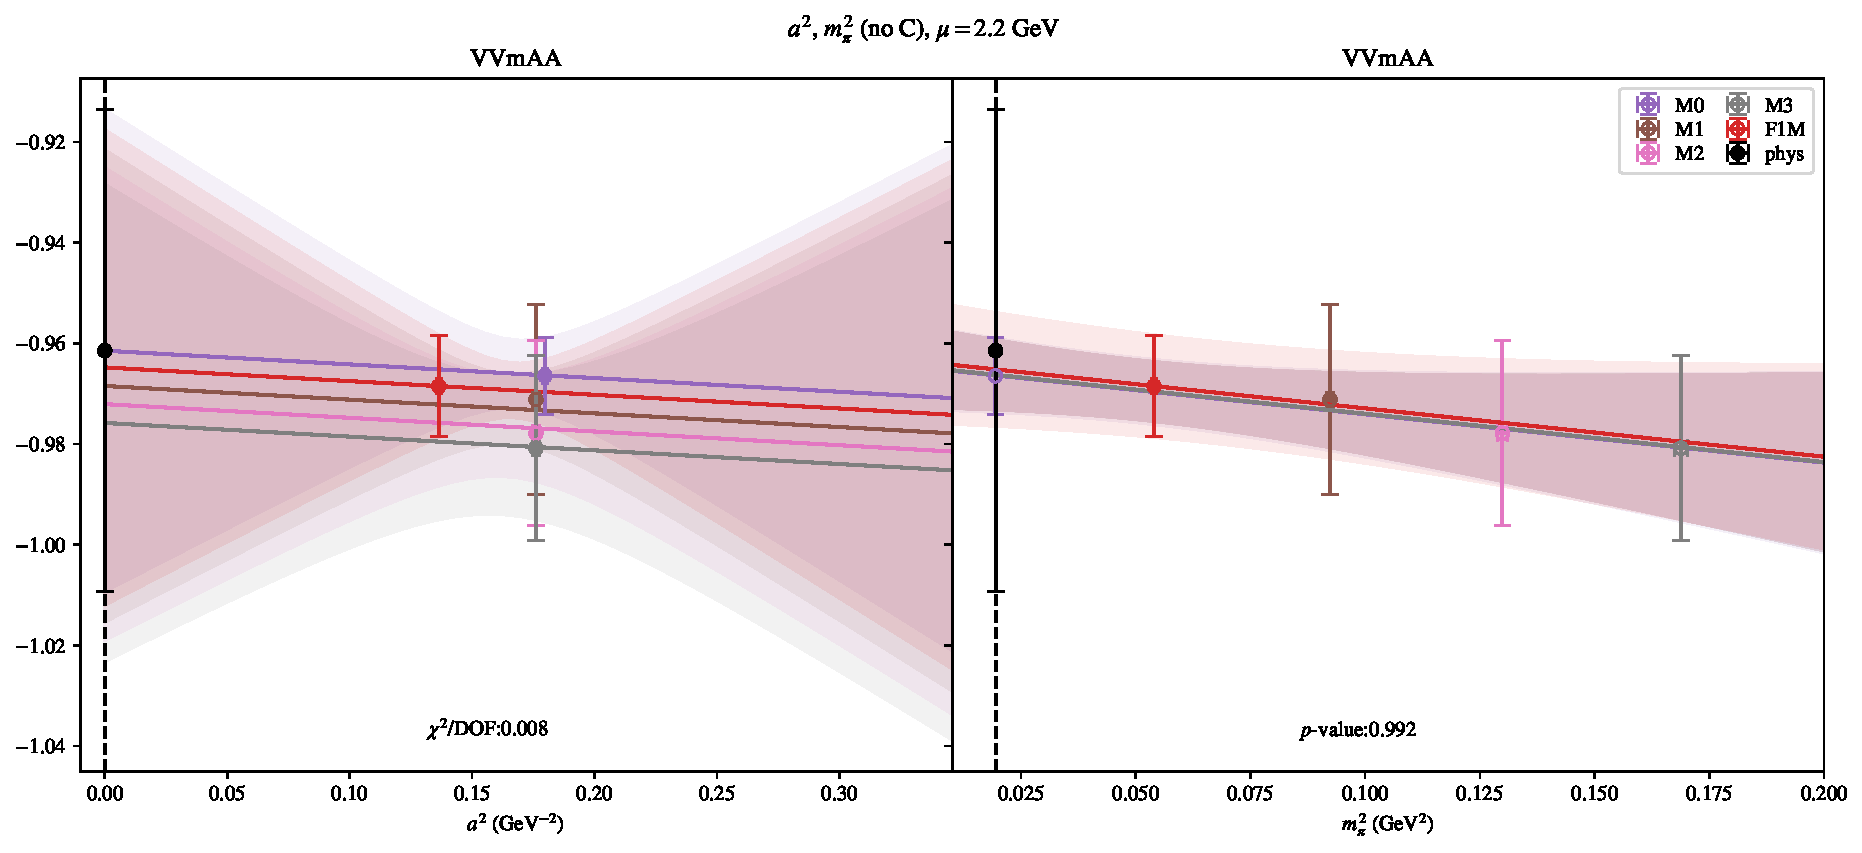
\includepdf[link, pages=-]{VVmAA/NPR/bag_a2m2noC_22.pdf}
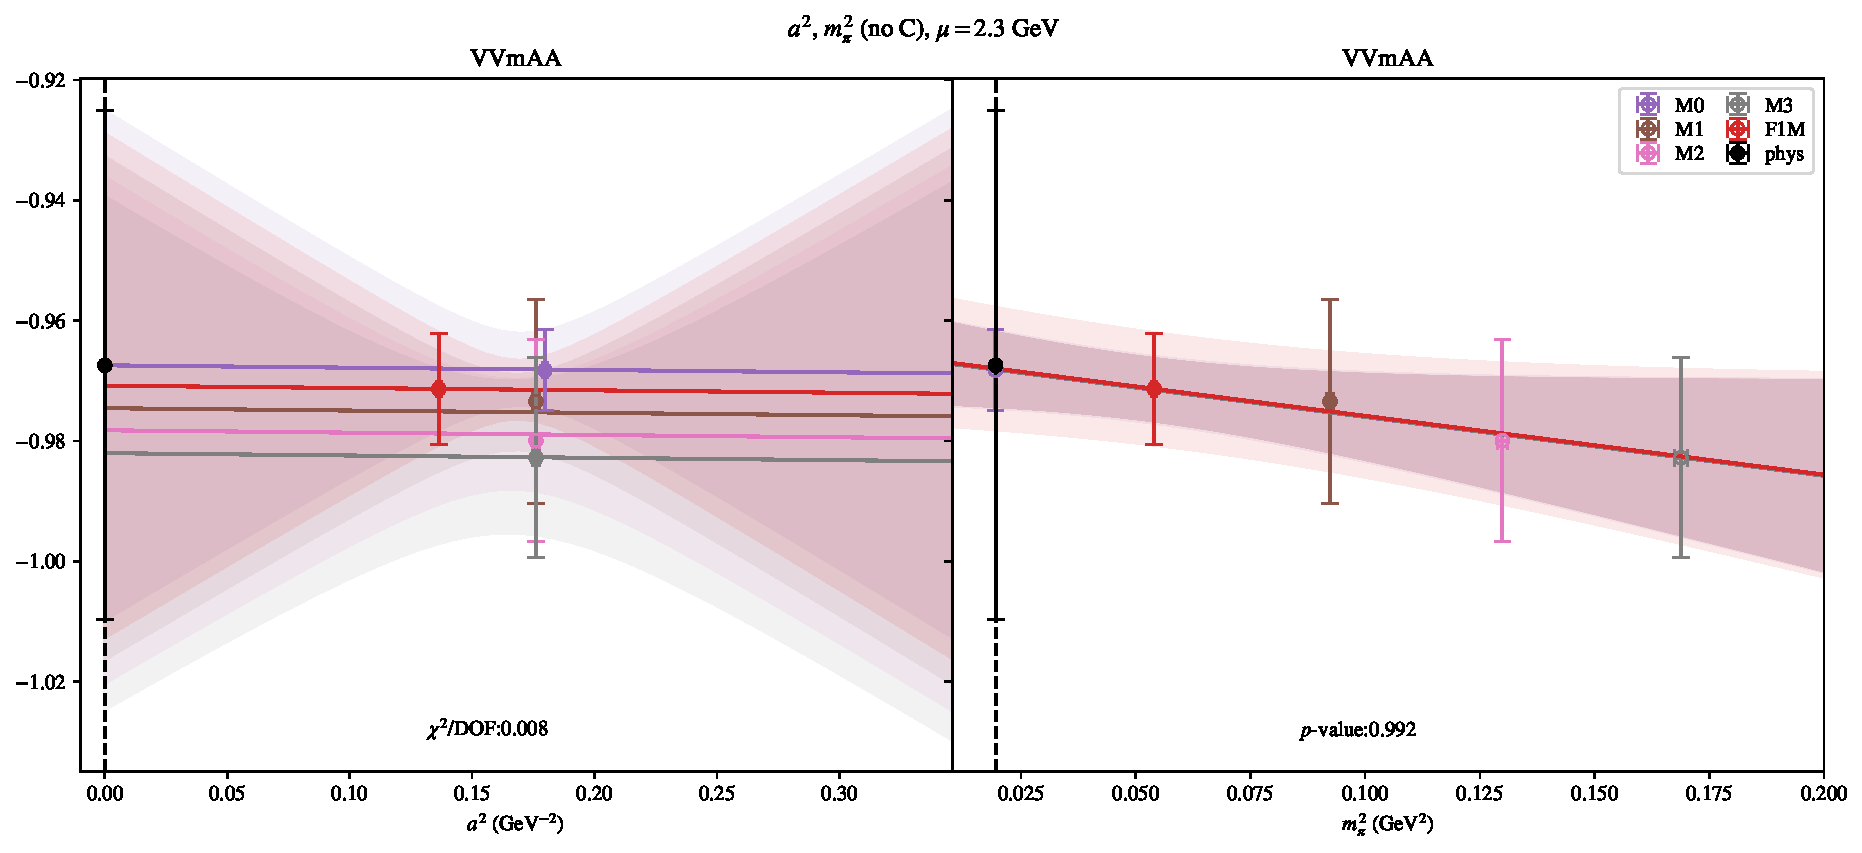
\includepdf[link, pages=-]{VVmAA/NPR/bag_a2m2noC_23.pdf}
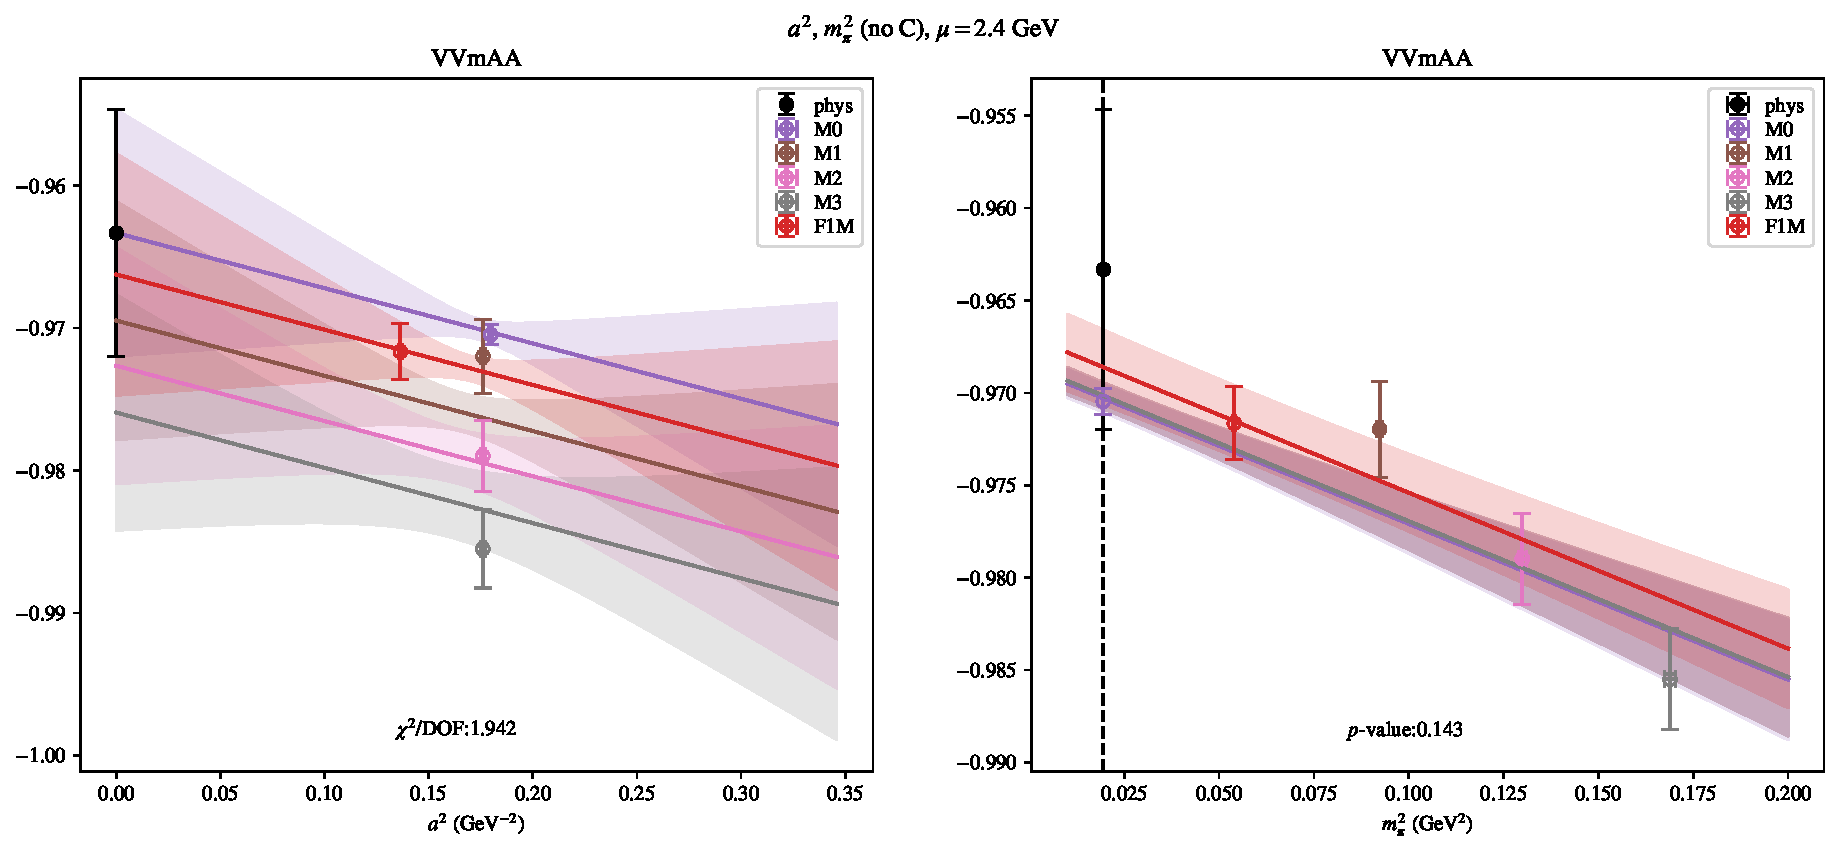
\includepdf[link, pages=-]{VVmAA/NPR/bag_a2m2noC_24.pdf}
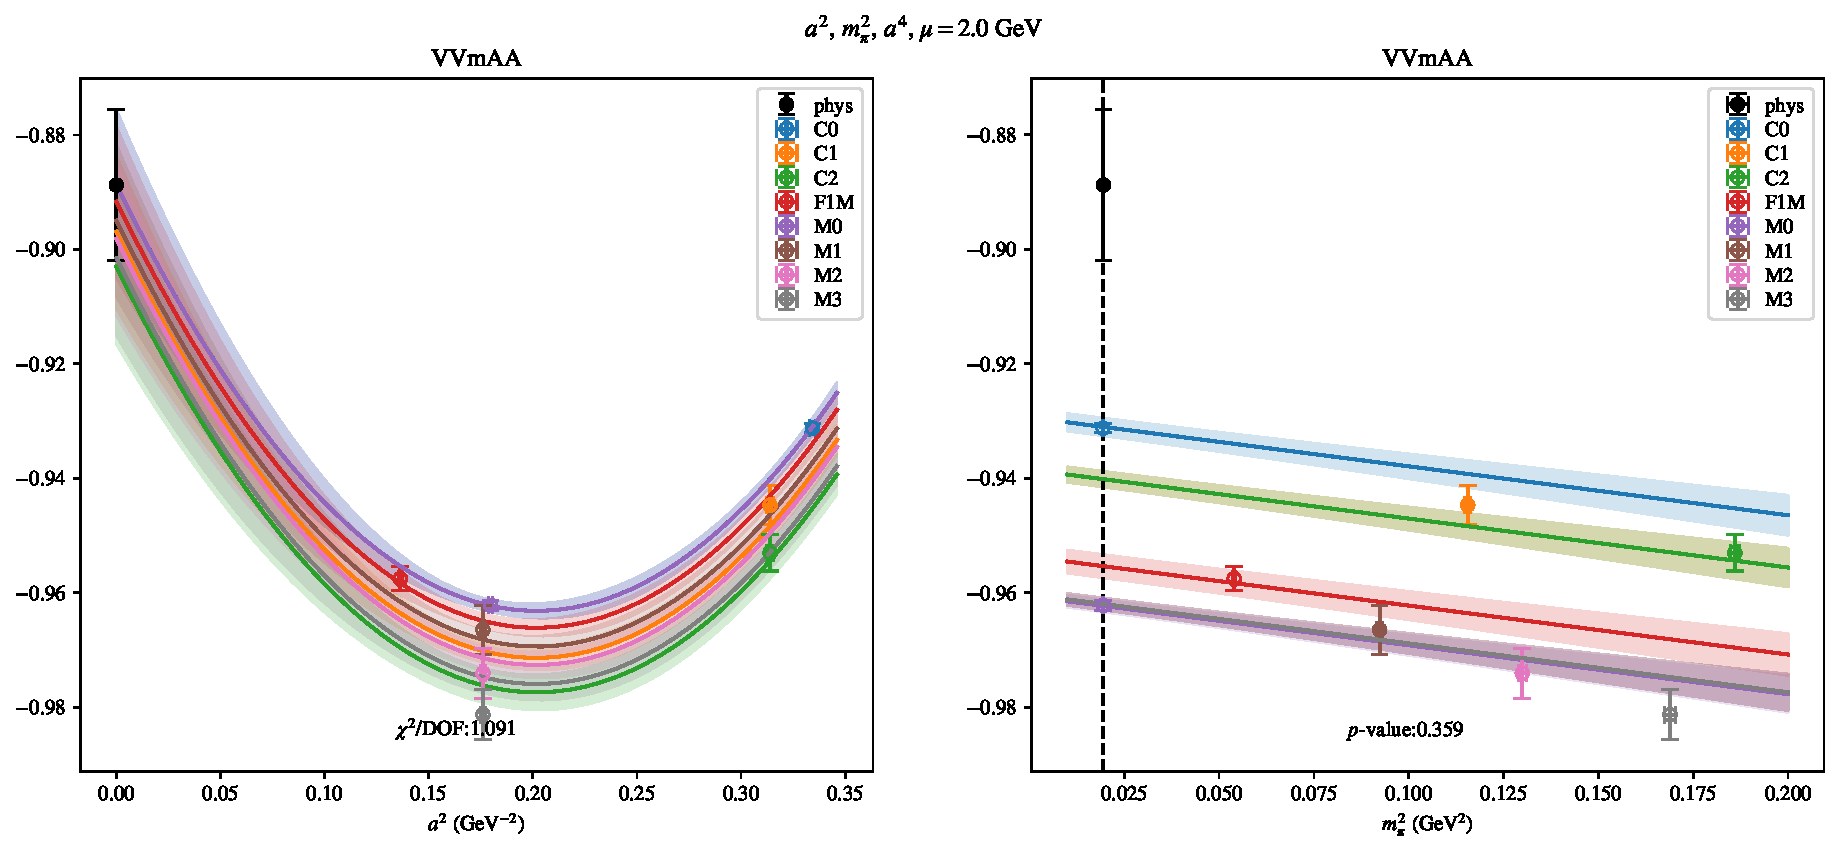
\includepdf[link, pages=-]{VVmAA/NPR/bag_a2a4m2_20.pdf}
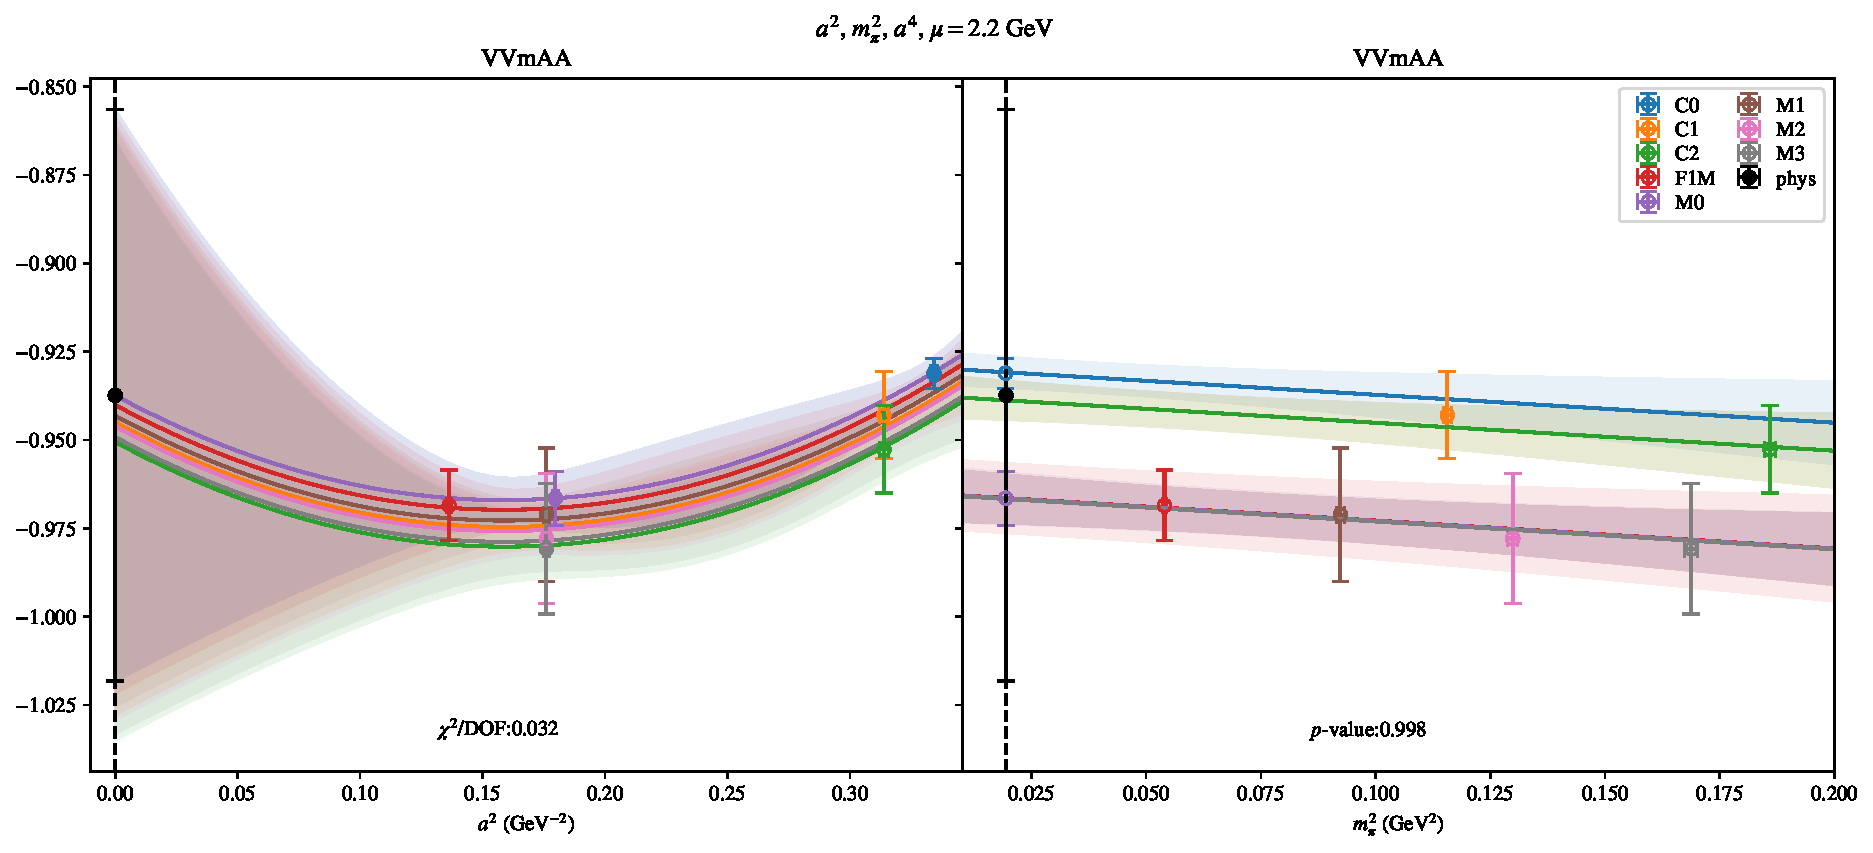
\includepdf[link, pages=-]{VVmAA/NPR/bag_a2a4m2_22.pdf}
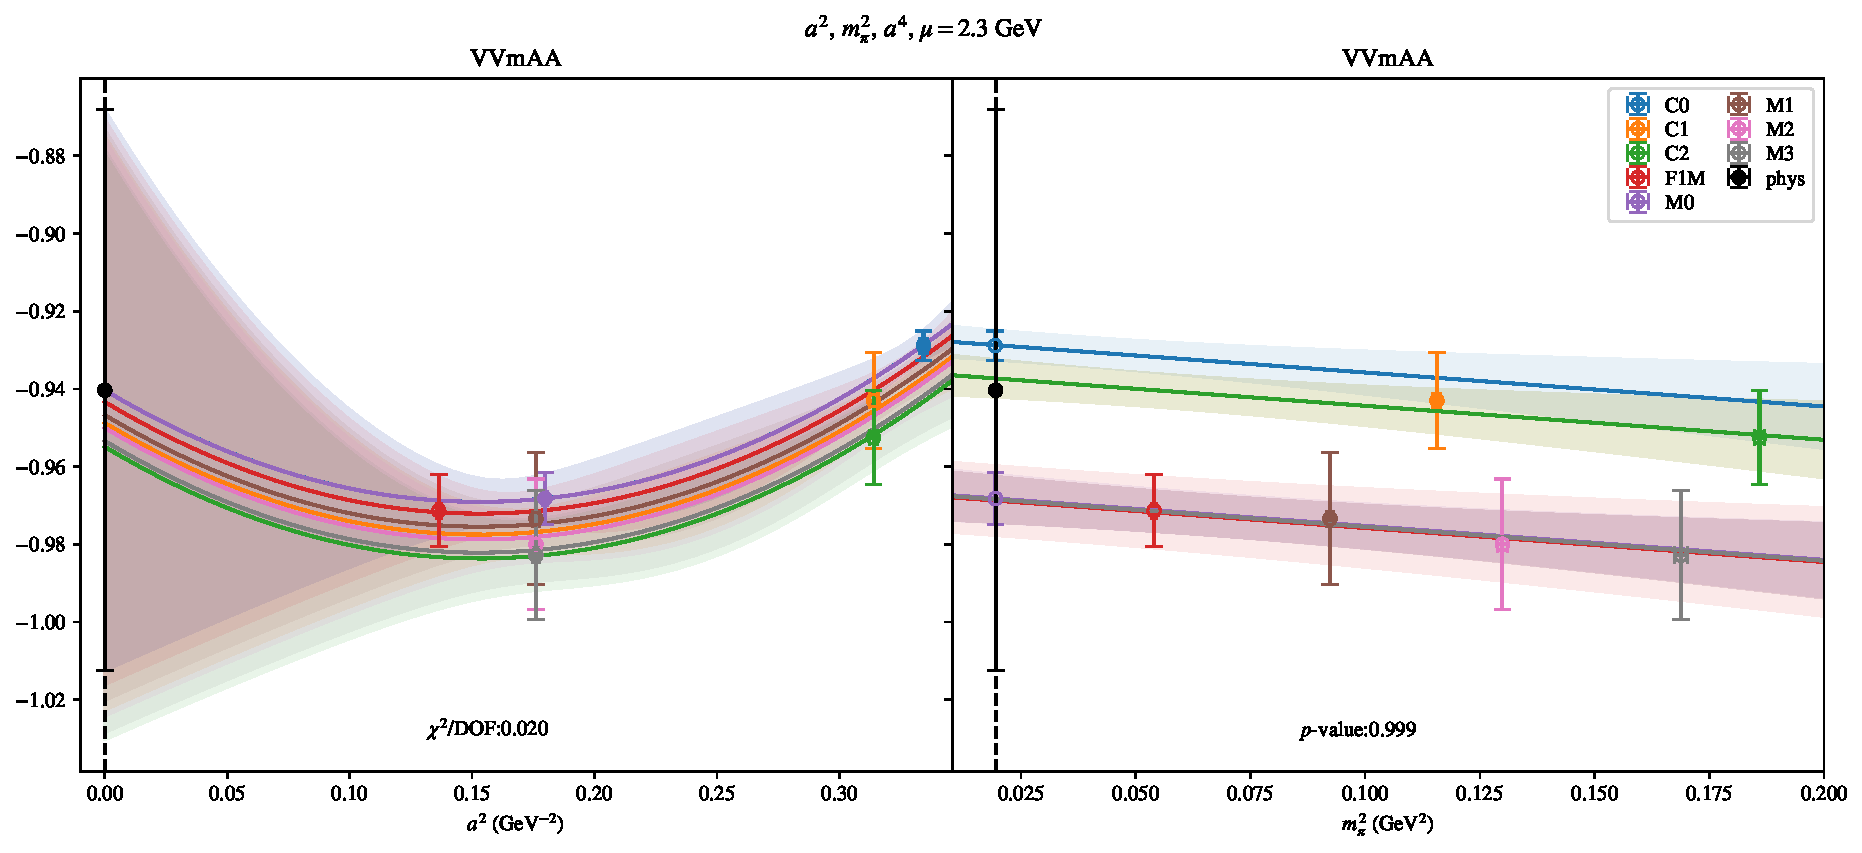
\includepdf[link, pages=-]{VVmAA/NPR/bag_a2a4m2_23.pdf}
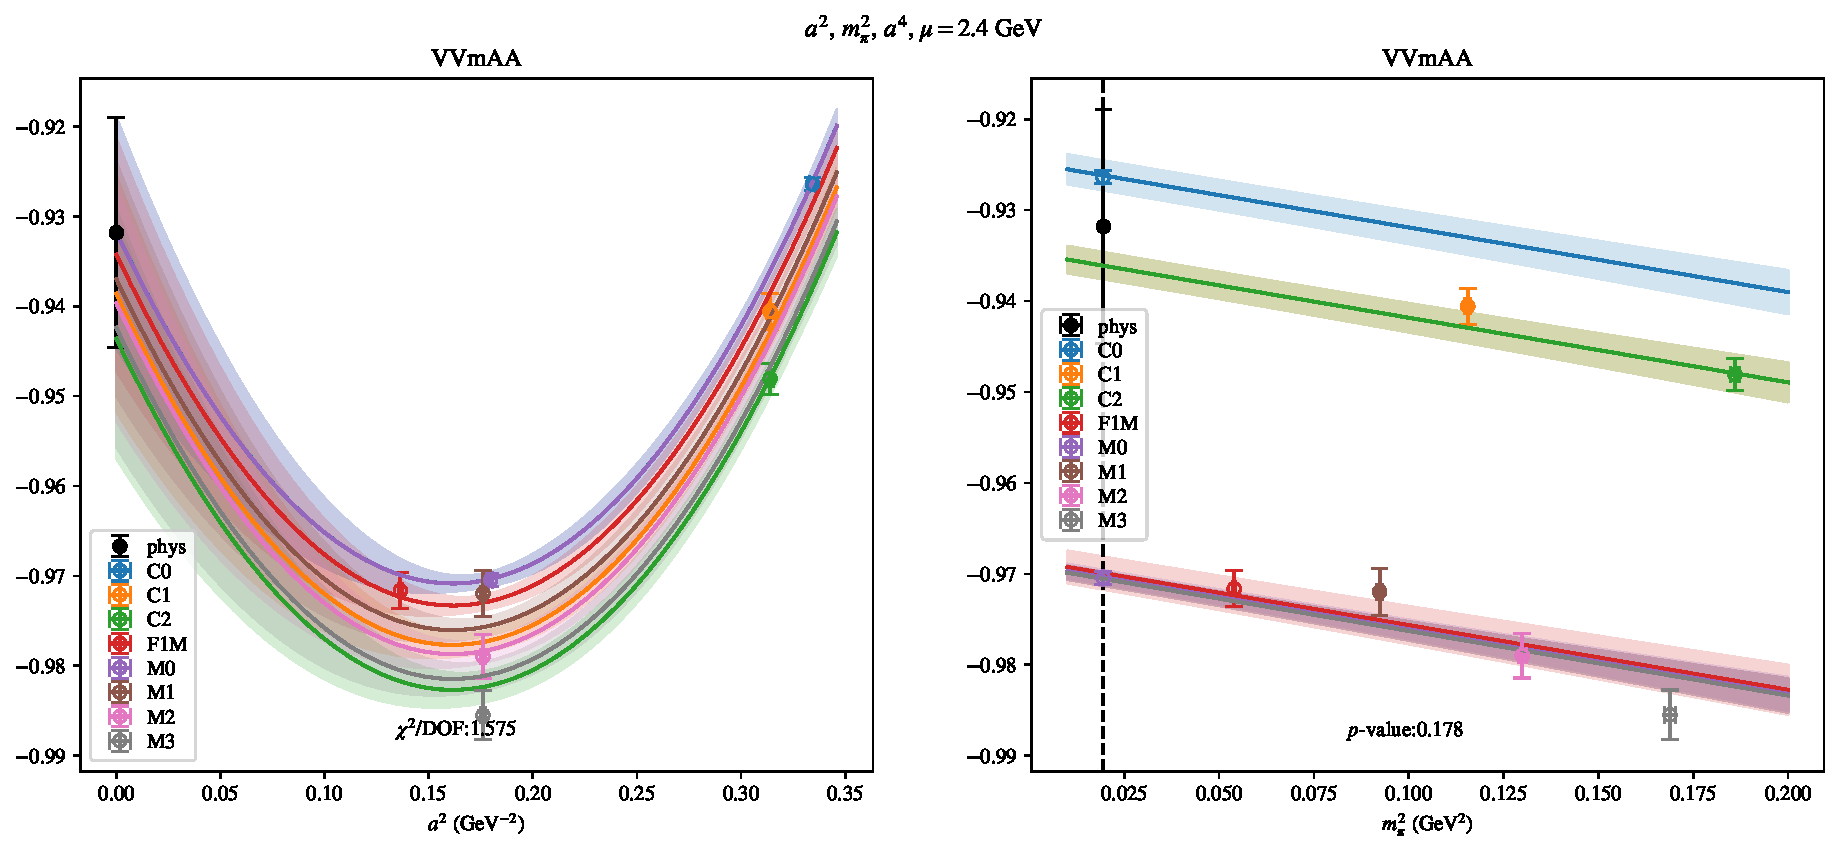
\includepdf[link, pages=-]{VVmAA/NPR/bag_a2a4m2_24.pdf}
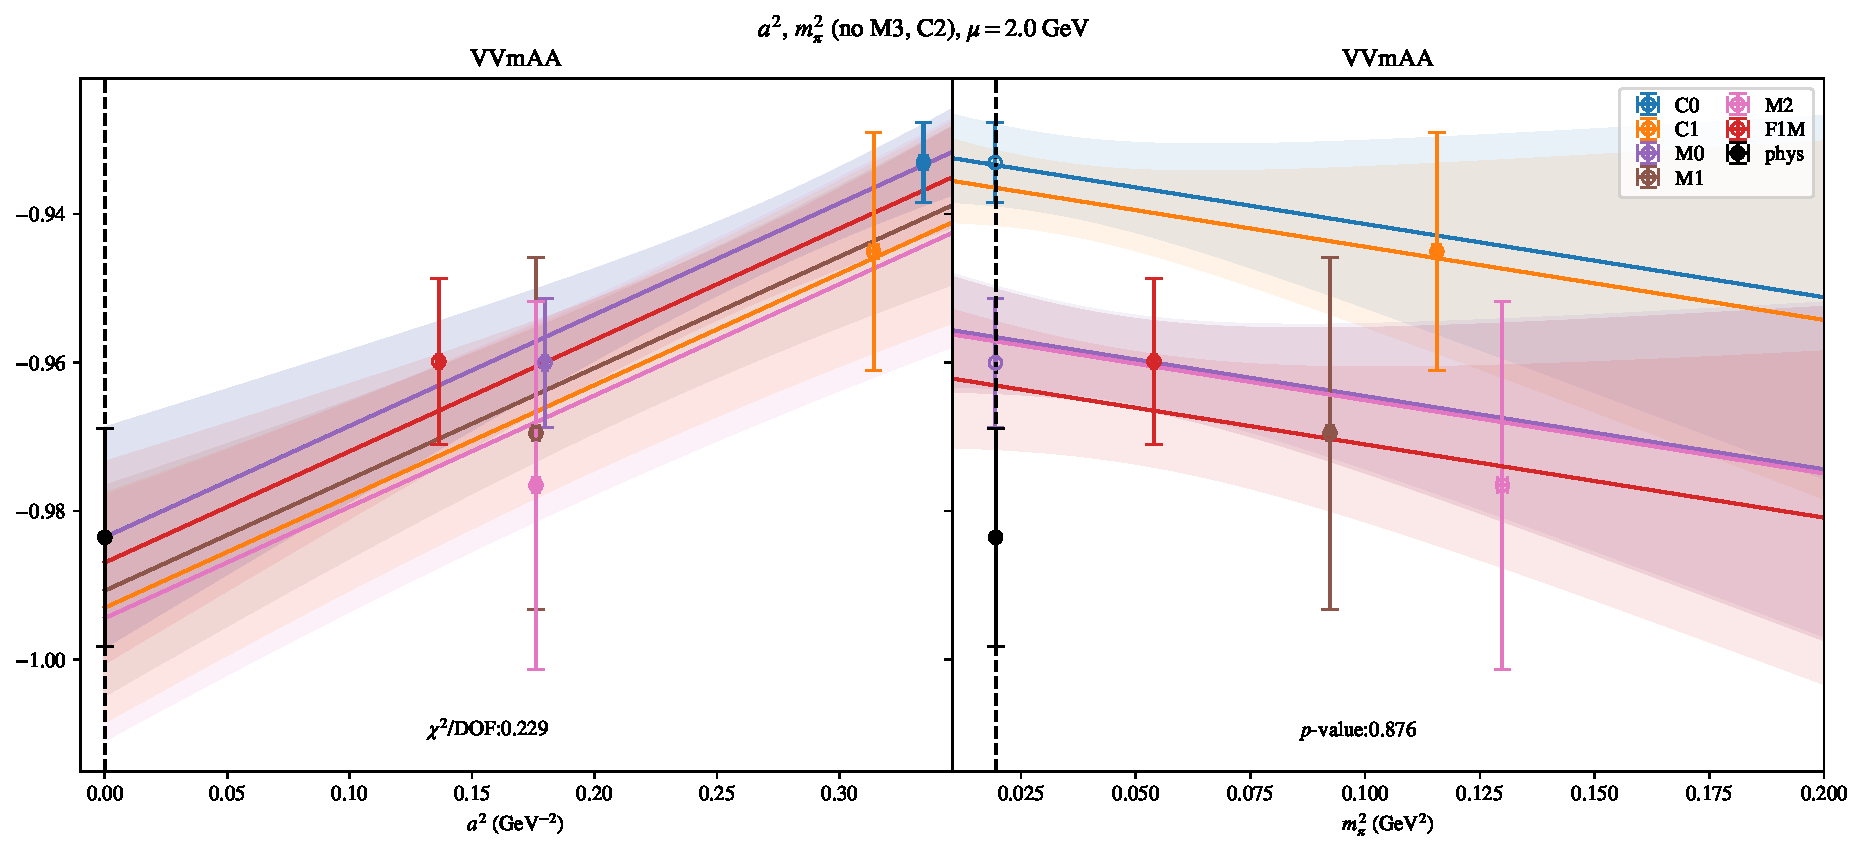
\includepdf[link, pages=-]{VVmAA/NPR/bag_a2m2mcut_20.pdf}
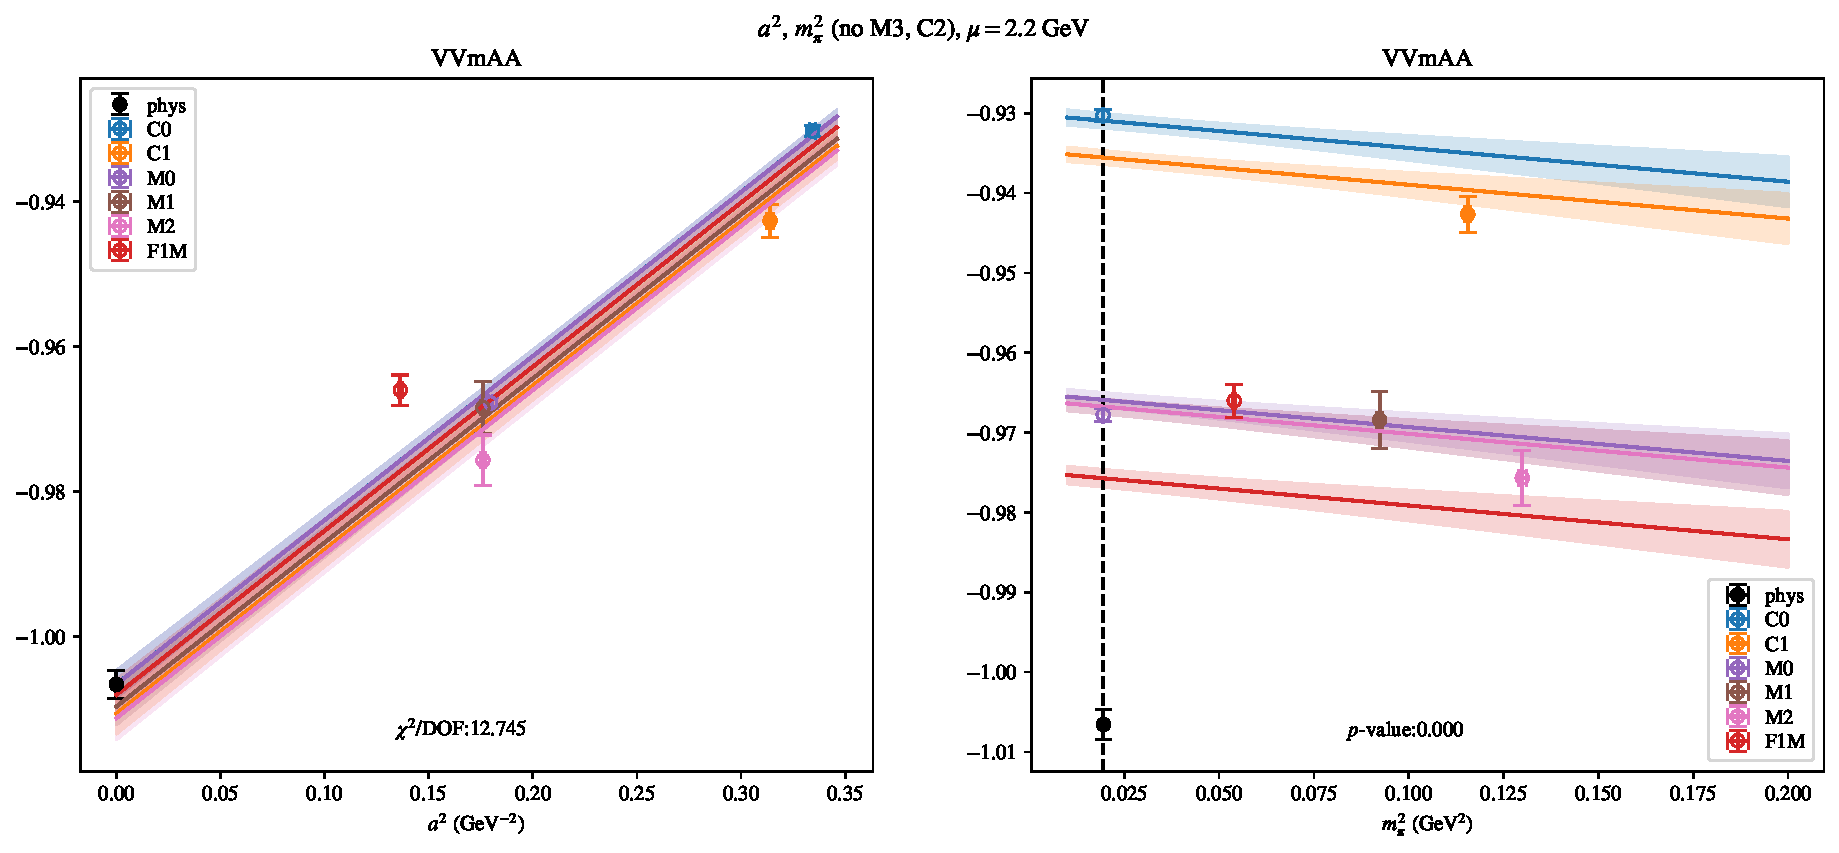
\includepdf[link, pages=-]{VVmAA/NPR/bag_a2m2mcut_22.pdf}
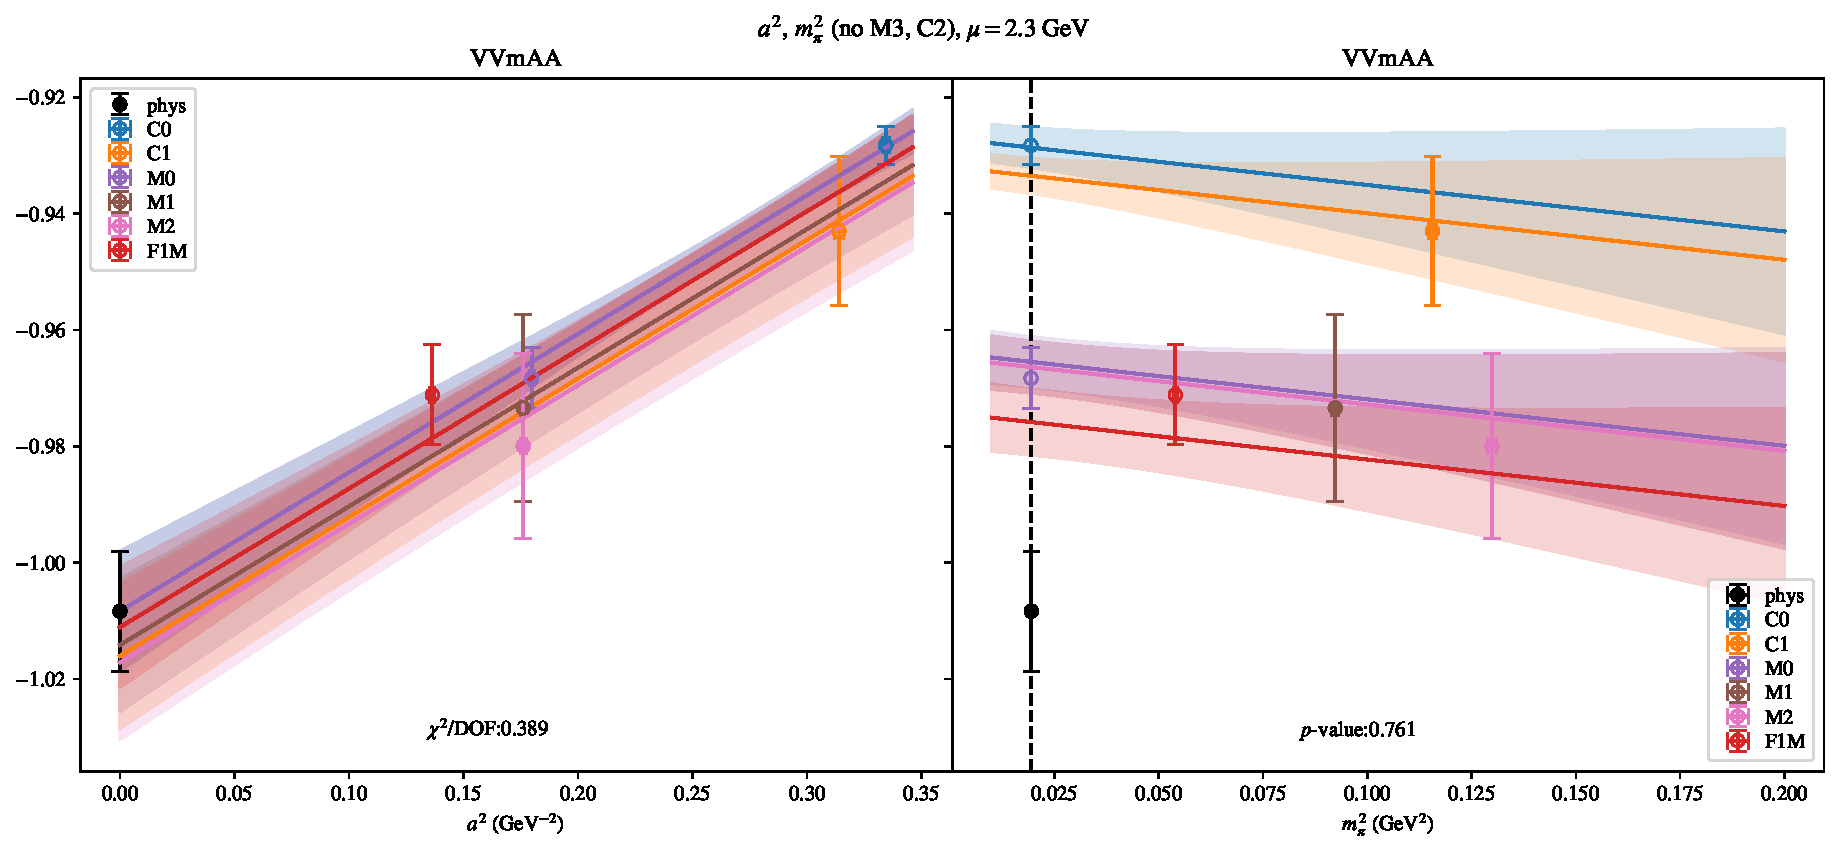
\includepdf[link, pages=-]{VVmAA/NPR/bag_a2m2mcut_23.pdf}
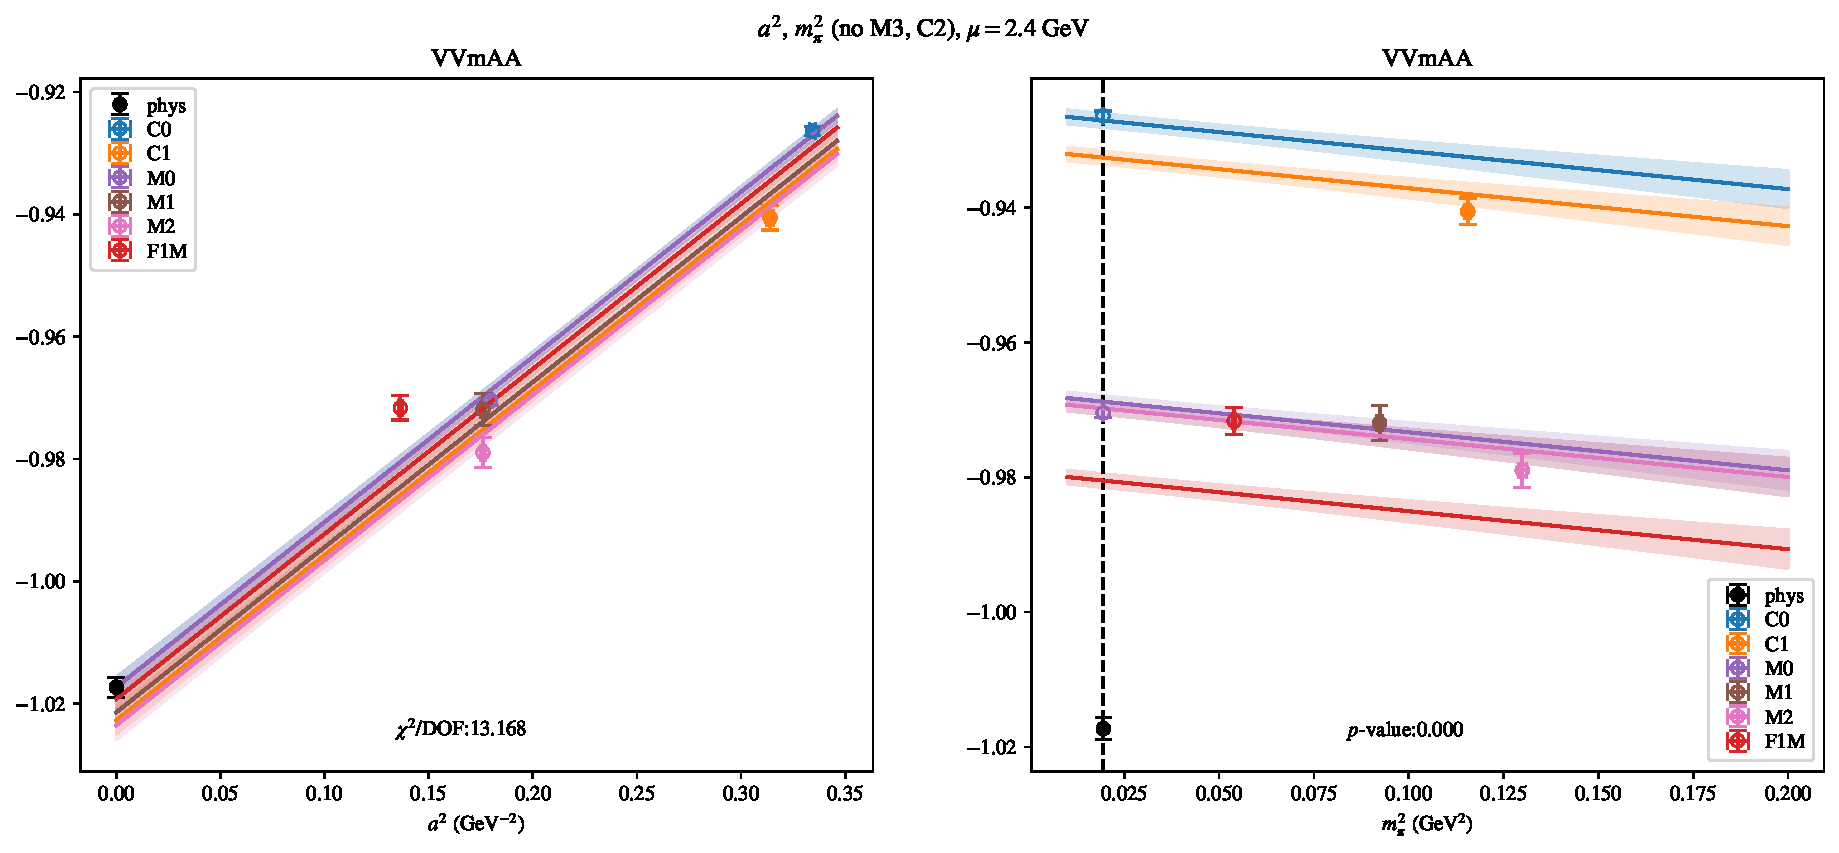
\includepdf[link, pages=-]{VVmAA/NPR/bag_a2m2mcut_24.pdf}
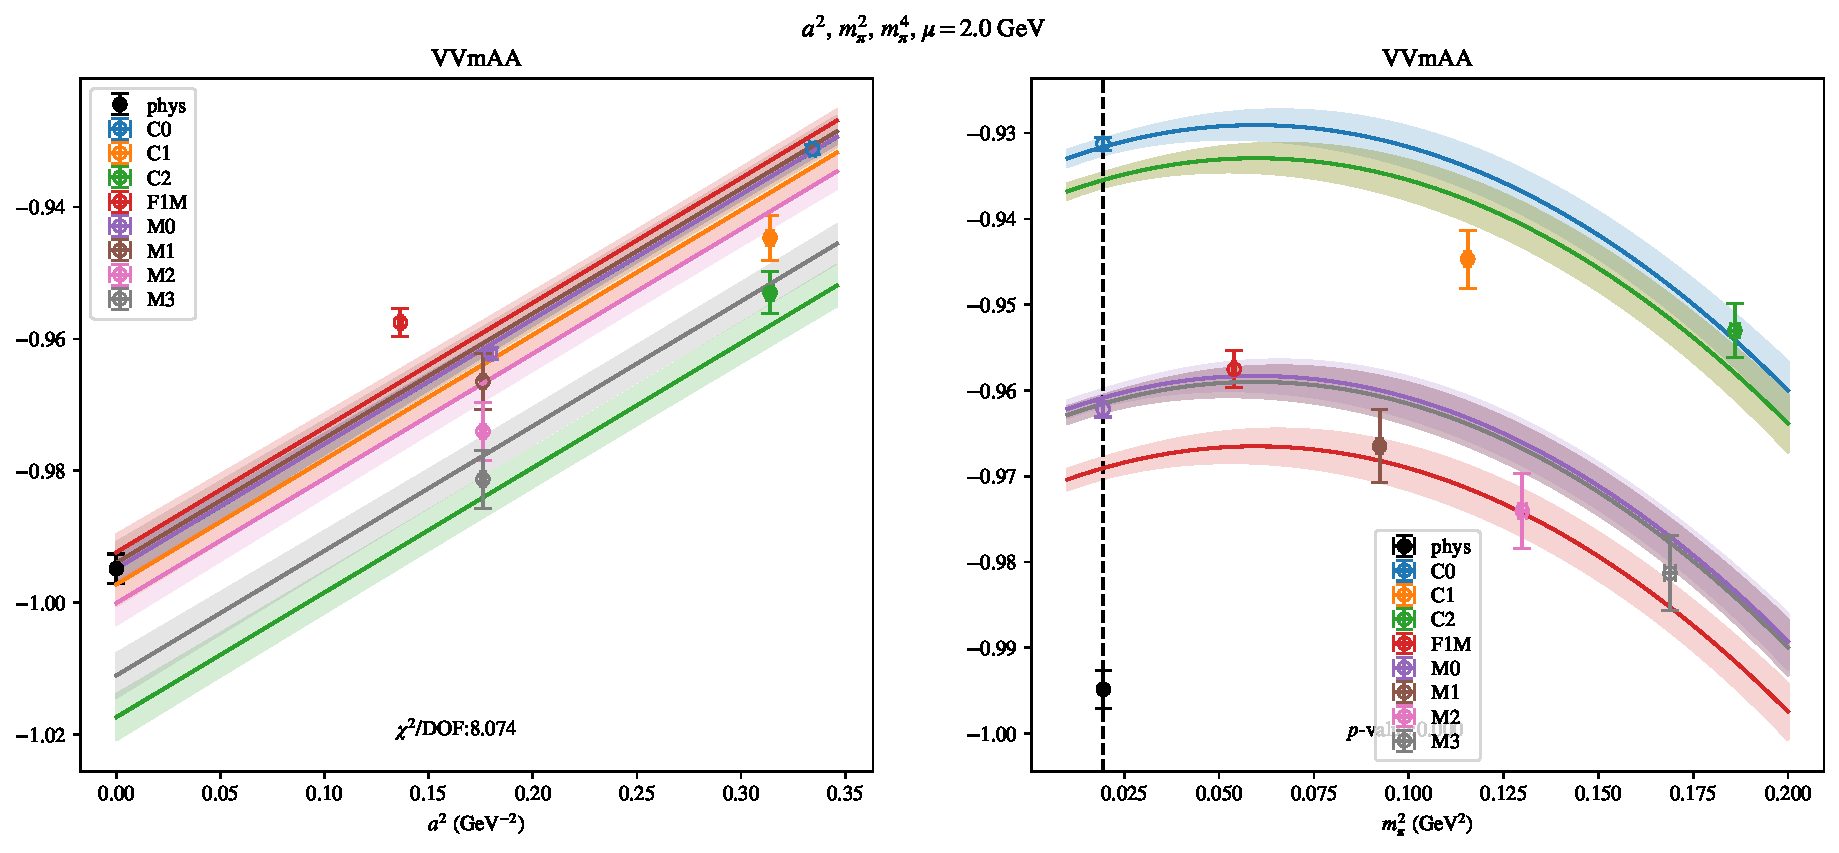
\includepdf[link, pages=-]{VVmAA/NPR/bag_a2m2m4_20.pdf}
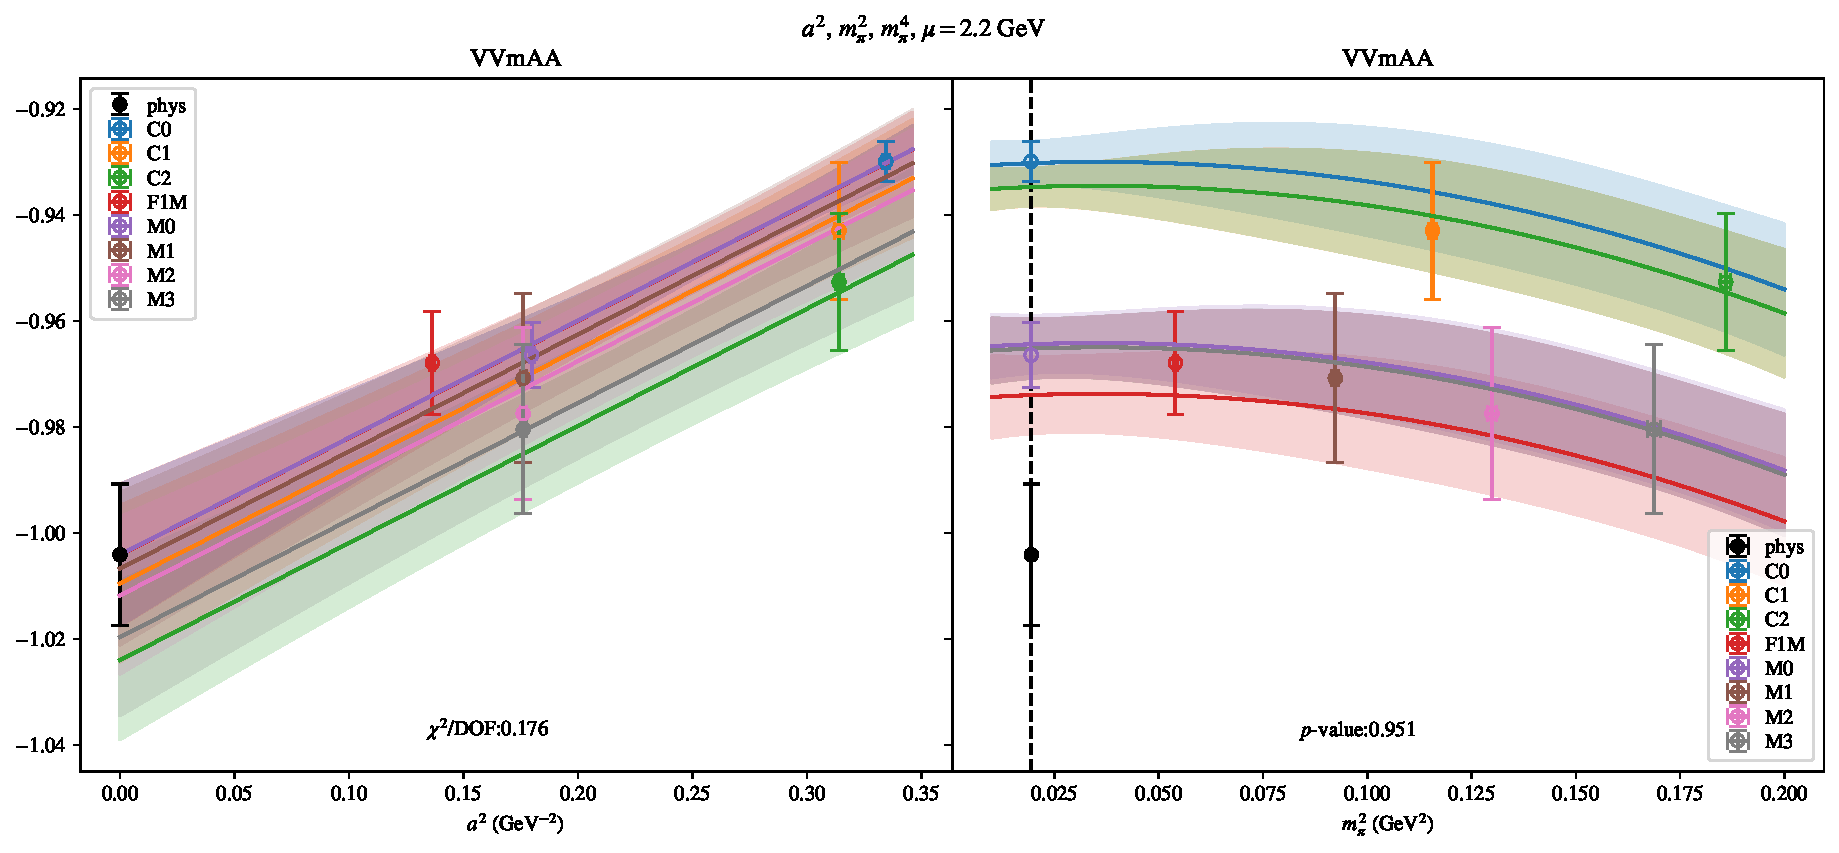
\includepdf[link, pages=-]{VVmAA/NPR/bag_a2m2m4_22.pdf}
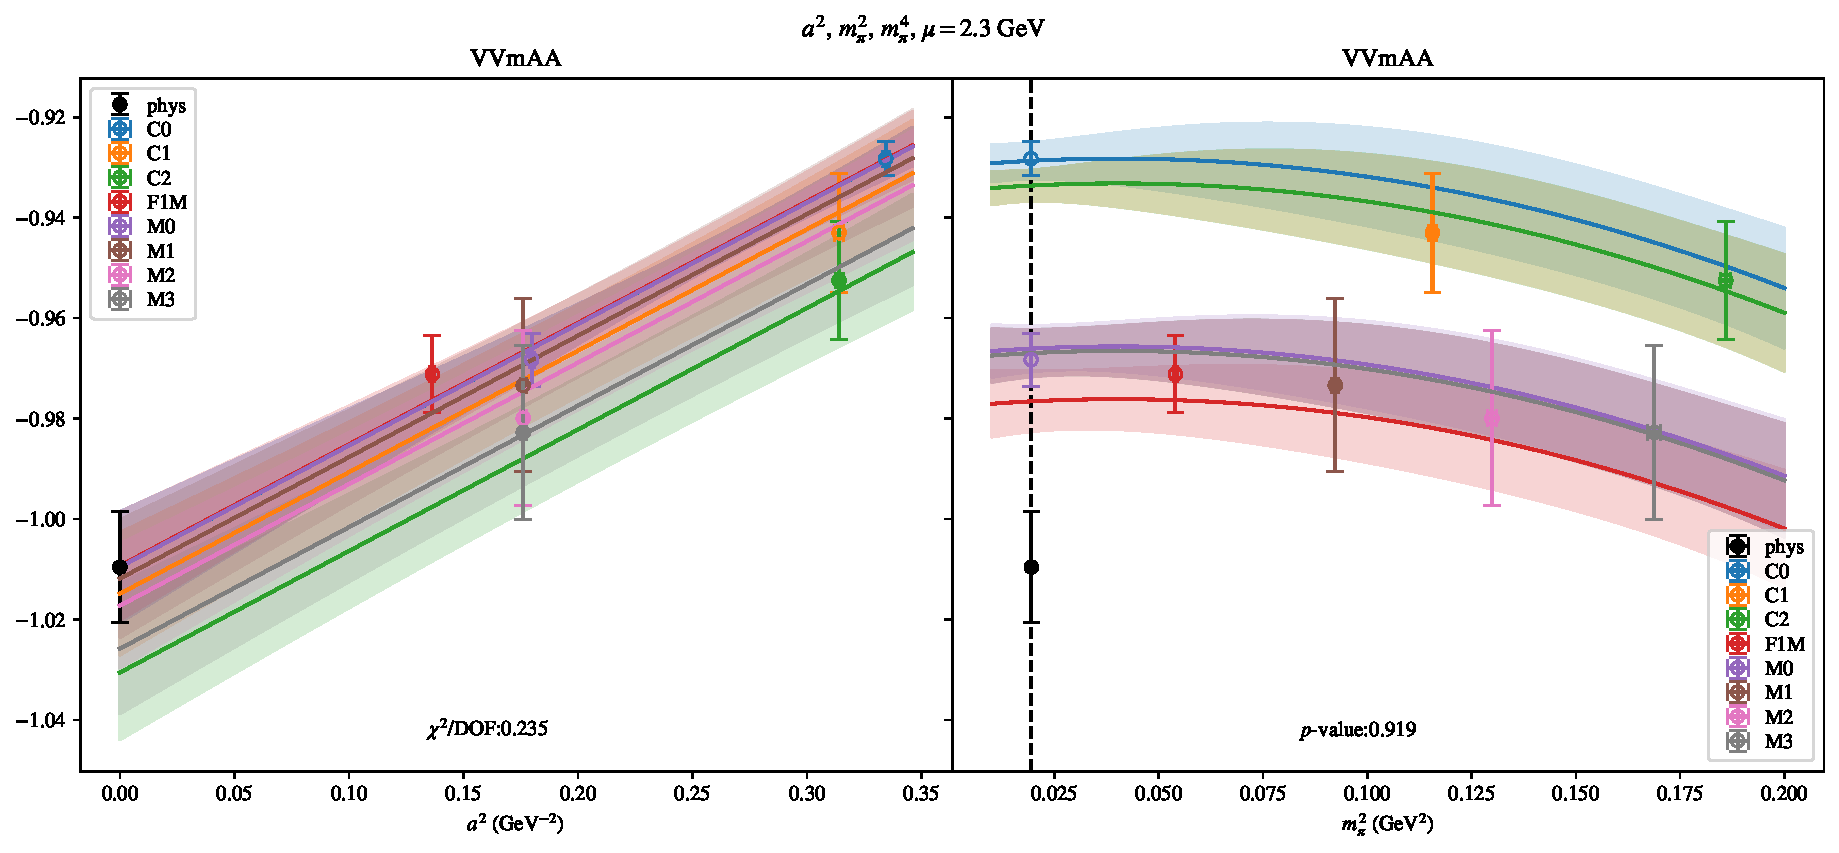
\includepdf[link, pages=-]{VVmAA/NPR/bag_a2m2m4_23.pdf}
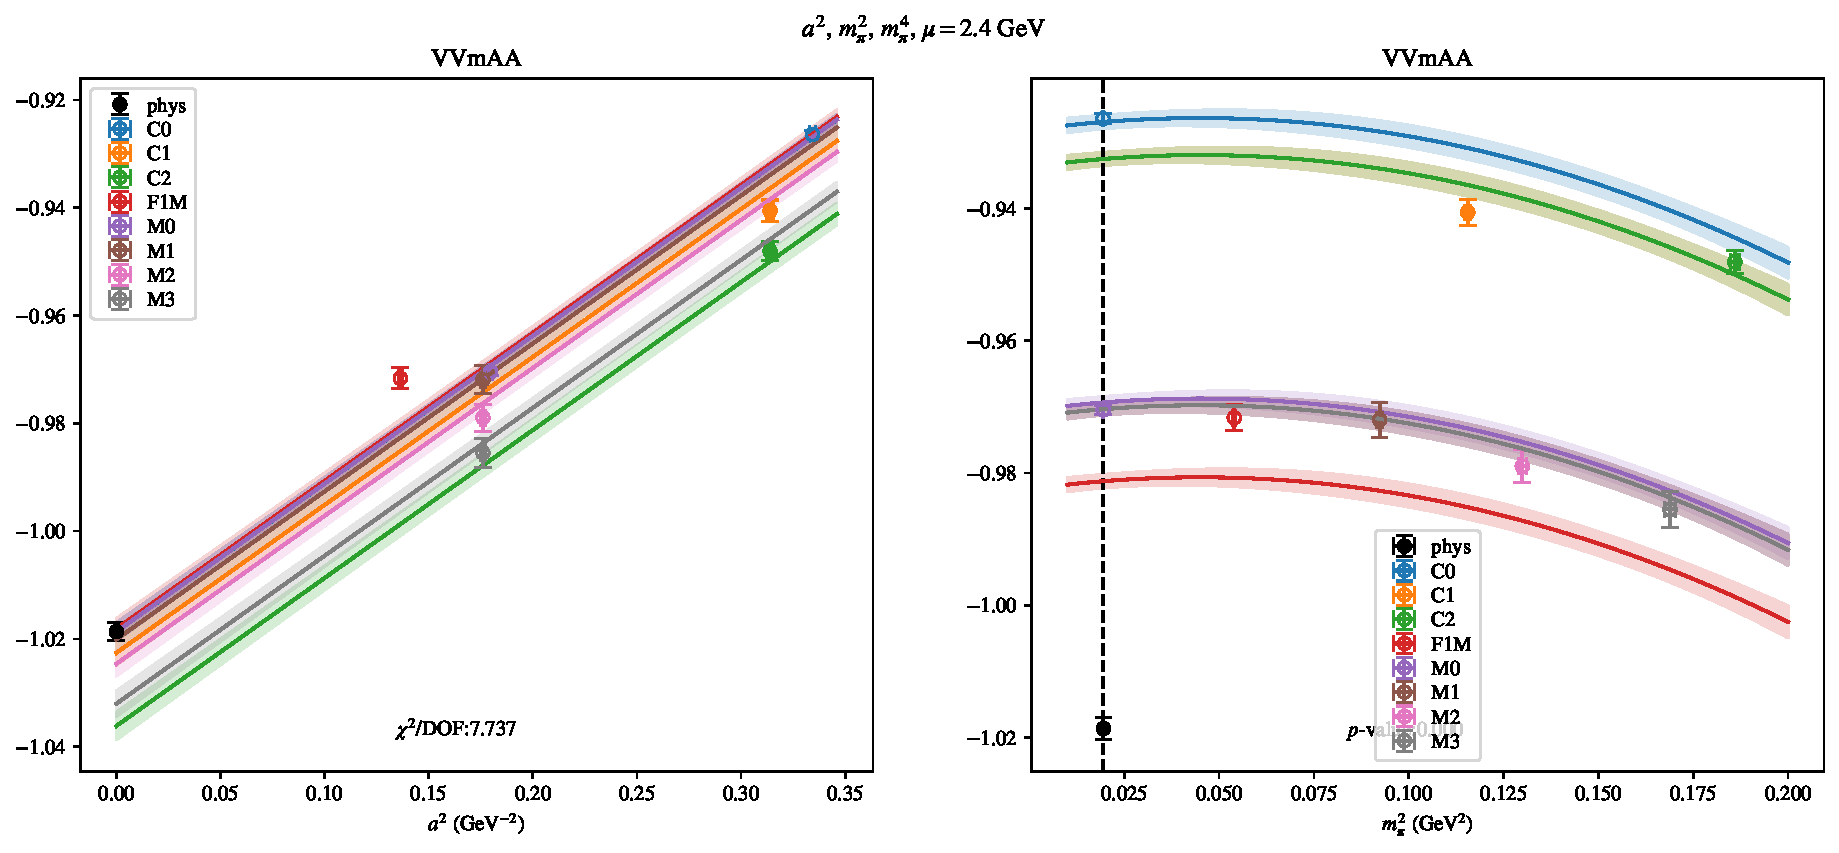
\includepdf[link, pages=-]{VVmAA/NPR/bag_a2m2m4_24.pdf}
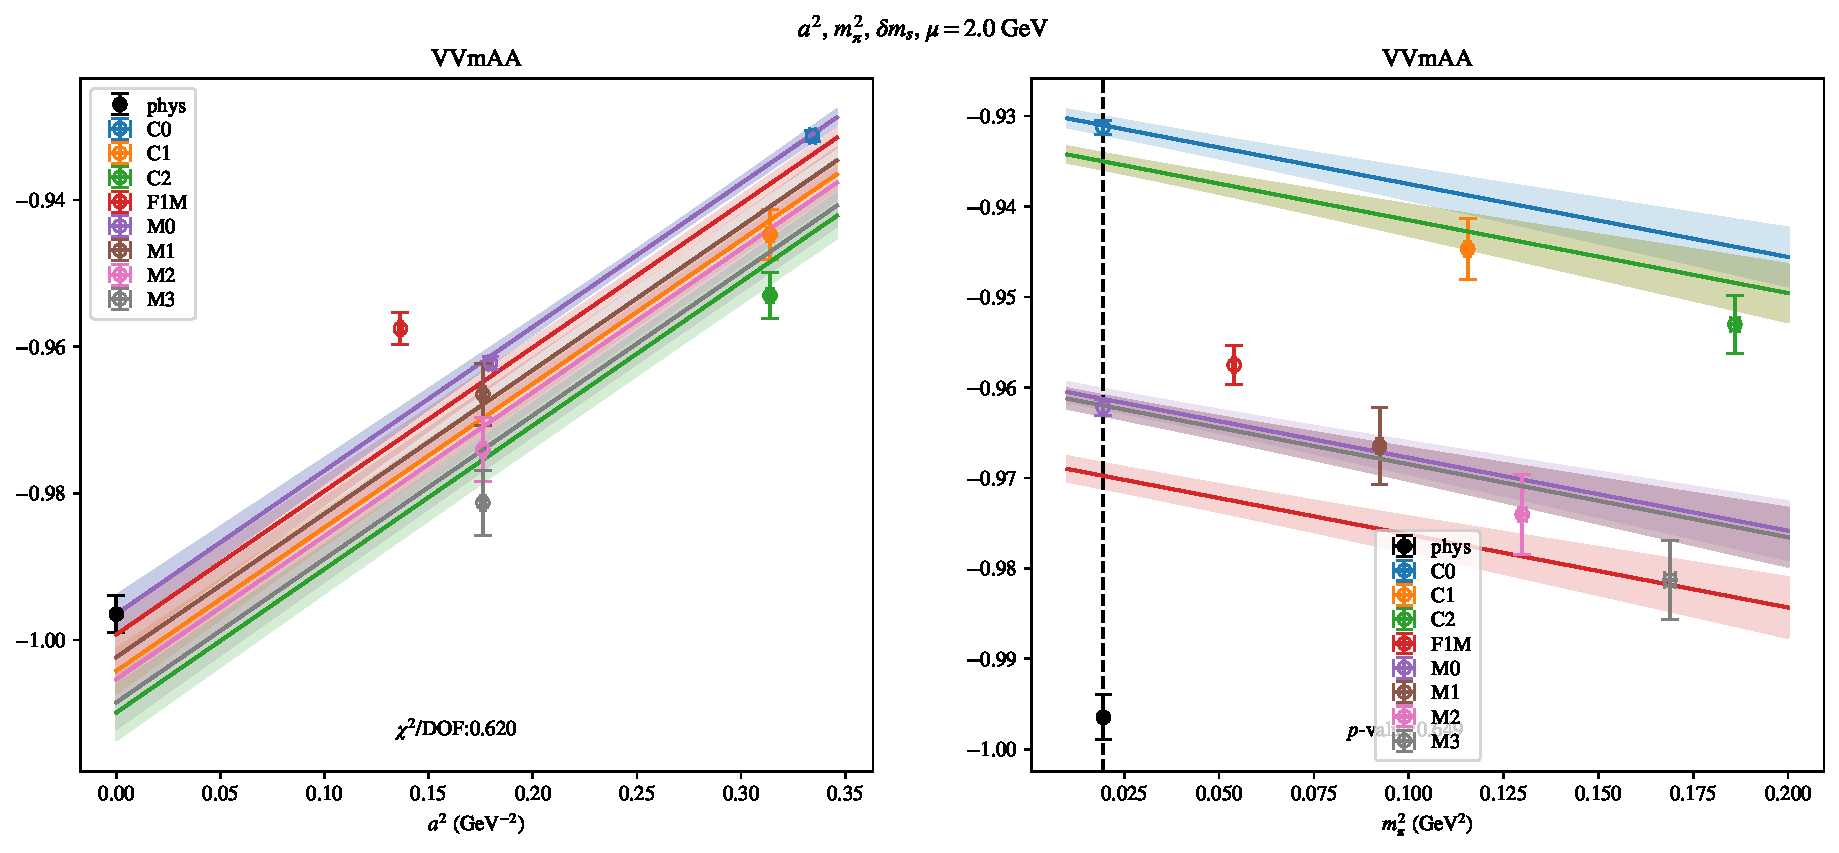
\includepdf[link, pages=-]{VVmAA/NPR/bag_a2m2delm_20.pdf}
\includepdf[link, pages=-]{VVmAA/NPR/bag_a2m2delm_22.pdf}
\includepdf[link, pages=-]{VVmAA/NPR/bag_a2m2delm_23.pdf}
\includepdf[link, pages=-]{VVmAA/NPR/bag_a2m2delm_24.pdf}
\clearpage
\section{$\mathcal{B}_3$}
\begin{table}[h!]
\begin{center}
\begin{tabular}{|c|c|c|c|c|c|c|}
\hline
$\mu$ (GeV) & $a^2$, $m_\pi^2$& $a^2$, $m_\pi^2$ (no C)& $a^2$, $m_\pi^2$, $a^4$& $a^2$, $m_\pi^2$ (no M3, C2)& $a^2$, $m_\pi^2$, $m_\pi^4$& $a^2$, $m_\pi^2$, $\delta m_s$\\
\hline
2.0& \hyperlink{SSmPP/NPR/bag_a2m2_20.pdf.1}{\textbf{1.8007(47)}: 6.529 (0.0)} & \hyperlink{SSmPP/NPR/bag_a2m2noC_20.pdf.1}{\textbf{1.696(22)}: 0.056 (0.945)} & \hyperlink{SSmPP/NPR/bag_a2a4m2_20.pdf.1}{\textbf{1.636(29)}: 0.781 (0.538)} & \hyperlink{SSmPP/NPR/bag_a2m2mcut_20.pdf.1}{\textbf{1.8007(46)}: 10.481 (0.0)} & \hyperlink{SSmPP/NPR/bag_a2m2m4_20.pdf.1}{\textbf{1.8044(54)}: 5.751 (0.0)} & \hyperlink{SSmPP/NPR/bag_a2m2delm_20.pdf.1}{\textbf{1.7979(57)}: 2.504 (0.04)}\\
2.2& \hyperlink{SSmPP/NPR/bag_a2m2_22.pdf.1}{\textbf{1.8027(37)}: 7.888 (0.0)} & \hyperlink{SSmPP/NPR/bag_a2m2noC_22.pdf.1}{\textbf{1.715(15)}: 0.131 (0.877)} & \hyperlink{SSmPP/NPR/bag_a2a4m2_22.pdf.1}{\textbf{1.662(24)}: 0.922 (0.45)} & \hyperlink{SSmPP/NPR/bag_a2m2mcut_22.pdf.1}{\textbf{1.8038(40)}: 12.13 (0.0)} & \hyperlink{SSmPP/NPR/bag_a2m2m4_22.pdf.1}{\textbf{1.8071(41)}: 6.957 (0.0)} & \hyperlink{SSmPP/NPR/bag_a2m2delm_22.pdf.1}{\textbf{1.8029(45)}: 4.336 (0.002)}\\
2.3& \hyperlink{SSmPP/NPR/bag_a2m2_23.pdf.1}{\textbf{1.8035(38)}: 8.265 (0.0)} & \hyperlink{SSmPP/NPR/bag_a2m2noC_23.pdf.1}{\textbf{1.721(15)}: 0.182 (0.834)} & \hyperlink{SSmPP/NPR/bag_a2a4m2_23.pdf.1}{\textbf{1.666(24)}: 0.734 (0.568)} & \hyperlink{SSmPP/NPR/bag_a2m2mcut_23.pdf.1}{\textbf{1.8042(37)}: 12.682 (0.0)} & \hyperlink{SSmPP/NPR/bag_a2m2m4_23.pdf.1}{\textbf{1.8083(38)}: 7.463 (0.0)} & \hyperlink{SSmPP/NPR/bag_a2m2delm_23.pdf.1}{\textbf{1.8034(43)}: 4.215 (0.002)}\\
2.4& \hyperlink{SSmPP/NPR/bag_a2m2_24.pdf.1}{\textbf{1.8049(35)}: 7.616 (0.0)} & \hyperlink{SSmPP/NPR/bag_a2m2noC_24.pdf.1}{\textbf{1.726(13)}: 0.241 (0.786)} & \hyperlink{SSmPP/NPR/bag_a2a4m2_24.pdf.1}{\textbf{1.674(22)}: 0.847 (0.495)} & \hyperlink{SSmPP/NPR/bag_a2m2mcut_24.pdf.1}{\textbf{1.8048(35)}: 13.79 (0.0)} & \hyperlink{SSmPP/NPR/bag_a2m2m4_24.pdf.1}{\textbf{1.8100(38)}: 7.591 (0.0)} & \hyperlink{SSmPP/NPR/bag_a2m2delm_24.pdf.1}{\textbf{1.8051(40)}: 4.347 (0.002)}\\
\hline
\end{tabular}
\caption{Physical point value from chiral and continuum extrapolation at renormalisation scale $\mu$. Entries are \textbf{value(error)}: $\chi^2/\text{DOF}$ ($p$-value).}
\end{center}
\end{table}
\begin{table}[h!]
\begin{center}
\begin{tabular}{|c c|c|c|c|c|c|c|}
\hline
$\mu$ (GeV) &  & $a^2$, $m_\pi^2$& $a^2$, $m_\pi^2$ (no C)& $a^2$, $m_\pi^2$, $a^4$& $a^2$, $m_\pi^2$ (no M3, C2)& $a^2$, $m_\pi^2$, $m_\pi^4$& $a^2$, $m_\pi^2$, $\delta m_s$\\
\hline
\multirow{3}{0.5in}{2.0} & $\alpha$ & 0.125(17)& 0.74(13)& 1.61(26)& 0.125(17)& 0.113(19)& 0.125(20)\\
 & $\beta$ & -0.00046(51)& 0.00015(96)& -0.00083(51)& -0.00114(79)& -0.0060(15)& -0.00381(84)\\
 & $\gamma$ &  &  & -2.98(53)&  & 0.00052(12)& 0.142(32)\\
\hline
\multirow{3}{0.5in}{2.2} & $\alpha$ & 0.143(13)& 0.666(91)& 1.43(22)& 0.140(14)& 0.129(14)& 0.136(16)\\
 & $\beta$ & -0.00066(32)& -0.00051(74)& -0.00123(34)& -0.00138(53)& -0.0054(13)& -0.00321(66)\\
 & $\gamma$ &  &  & -2.61(45)&  & 0.00043(11)& 0.099(23)\\
\hline
\multirow{3}{0.5in}{2.3} & $\alpha$ & 0.151(14)& 0.645(93)& 1.41(22)& 0.149(13)& 0.136(13)& 0.144(15)\\
 & $\beta$ & -0.00041(29)& -0.00049(65)& -0.00099(29)& -0.00092(49)& -0.0045(12)& -0.00297(62)\\
 & $\gamma$ &  &  & -2.56(45)&  & 0.00038(10)& 0.102(22)\\
\hline
\multirow{3}{0.5in}{2.4} & $\alpha$ & 0.154(12)& 0.629(82)& 1.36(20)& 0.155(13)& 0.138(13)& 0.147(14)\\
 & $\beta$ & -0.00033(27)& -0.00041(51)& -0.00090(27)& -0.00068(43)& -0.0037(12)& -0.00259(58)\\
 & $\gamma$ &  &  & -2.45(41)&  & 0.00031(10)& 0.090(21)\\
\hline
\end{tabular}
\caption{Fit values of coefficients in $Q = Q_{phys} + \mathbf{\alpha} a^2 + \mathbf{\beta}\left(\frac{m_\pi^2}{f_\pi^2}-\frac{m_{\pi,PDG}^2}{f_\pi^2}\right) + \gamma(\ldots)$}
\end{center}
\end{table}
\includepdf[link, pages=-]{SSmPP/NPR/bag_a2m2_20.pdf}
\includepdf[link, pages=-]{SSmPP/NPR/bag_a2m2_22.pdf}
\includepdf[link, pages=-]{SSmPP/NPR/bag_a2m2_23.pdf}
\includepdf[link, pages=-]{SSmPP/NPR/bag_a2m2_24.pdf}
\includepdf[link, pages=-]{SSmPP/NPR/bag_a2m2noC_20.pdf}
\includepdf[link, pages=-]{SSmPP/NPR/bag_a2m2noC_22.pdf}
\includepdf[link, pages=-]{SSmPP/NPR/bag_a2m2noC_23.pdf}
\includepdf[link, pages=-]{SSmPP/NPR/bag_a2m2noC_24.pdf}
\includepdf[link, pages=-]{SSmPP/NPR/bag_a2a4m2_20.pdf}
\includepdf[link, pages=-]{SSmPP/NPR/bag_a2a4m2_22.pdf}
\includepdf[link, pages=-]{SSmPP/NPR/bag_a2a4m2_23.pdf}
\includepdf[link, pages=-]{SSmPP/NPR/bag_a2a4m2_24.pdf}
\includepdf[link, pages=-]{SSmPP/NPR/bag_a2m2mcut_20.pdf}
\includepdf[link, pages=-]{SSmPP/NPR/bag_a2m2mcut_22.pdf}
\includepdf[link, pages=-]{SSmPP/NPR/bag_a2m2mcut_23.pdf}
\includepdf[link, pages=-]{SSmPP/NPR/bag_a2m2mcut_24.pdf}
\includepdf[link, pages=-]{SSmPP/NPR/bag_a2m2m4_20.pdf}
\includepdf[link, pages=-]{SSmPP/NPR/bag_a2m2m4_22.pdf}
\includepdf[link, pages=-]{SSmPP/NPR/bag_a2m2m4_23.pdf}
\includepdf[link, pages=-]{SSmPP/NPR/bag_a2m2m4_24.pdf}
\includepdf[link, pages=-]{SSmPP/NPR/bag_a2m2delm_20.pdf}
\includepdf[link, pages=-]{SSmPP/NPR/bag_a2m2delm_22.pdf}
\includepdf[link, pages=-]{SSmPP/NPR/bag_a2m2delm_23.pdf}
\includepdf[link, pages=-]{SSmPP/NPR/bag_a2m2delm_24.pdf}
\clearpage
\section{$\mathcal{B}_4$}
\begin{table}[h!]
\begin{center}
\begin{tabular}{|c|c|c|c|c|c|c|}
\hline
$\mu$ (GeV) & $a^2$, $m_\pi^2$& $a^2$, $m_\pi^2$ (no C)& $a^2$, $m_\pi^2$, $a^4$& $a^2$, $m_\pi^2$ (no M3, C2)& $a^2$, $m_\pi^2$, $m_\pi^4$& $a^2$, $m_\pi^2$, $\delta m_s$\\
\hline
2.0& \hyperlink{SSpPP/NPR/bag_a2m2_20.pdf.1}{\textbf{-0.9279(30)}: 0.929 (0.461)} & \hyperlink{SSpPP/NPR/bag_a2m2noC_20.pdf.1}{\textbf{-0.940(13)}: 0.798 (0.45)} & \hyperlink{SSpPP/NPR/bag_a2a4m2_20.pdf.1}{\textbf{-0.945(17)}: 0.962 (0.427)} & \hyperlink{SSpPP/NPR/bag_a2m2mcut_20.pdf.1}{\textbf{-0.9268(25)}: 0.661 (0.576)} & \hyperlink{SSpPP/NPR/bag_a2m2m4_20.pdf.1}{\textbf{-0.9257(27)}: 0.239 (0.916)} & \hyperlink{SSpPP/NPR/bag_a2m2delm_20.pdf.1}{\textbf{-0.9277(29)}: 1.187 (0.314)}\\
2.2& \hyperlink{SSpPP/NPR/bag_a2m2_22.pdf.1}{\textbf{-0.9077(21)}: 2.175 (0.054)} & \hyperlink{SSpPP/NPR/bag_a2m2noC_22.pdf.1}{\textbf{-0.9271(95)}: 0.828 (0.437)} & \hyperlink{SSpPP/NPR/bag_a2a4m2_22.pdf.1}{\textbf{-0.929(15)}: 2.097 (0.078)} & \hyperlink{SSpPP/NPR/bag_a2m2mcut_22.pdf.1}{\textbf{-0.9069(20)}: 1.885 (0.13)} & \hyperlink{SSpPP/NPR/bag_a2m2m4_22.pdf.1}{\textbf{-0.9057(21)}: 1.086 (0.361)} & \hyperlink{SSpPP/NPR/bag_a2m2delm_22.pdf.1}{\textbf{-0.9078(24)}: 2.634 (0.032)}\\
2.3& \hyperlink{SSpPP/NPR/bag_a2m2_23.pdf.1}{\textbf{-0.8986(20)}: 3.476 (0.004)} & \hyperlink{SSpPP/NPR/bag_a2m2noC_23.pdf.1}{\textbf{-0.9206(95)}: 1.053 (0.349)} & \hyperlink{SSpPP/NPR/bag_a2a4m2_23.pdf.1}{\textbf{-0.923(13)}: 3.113 (0.014)} & \hyperlink{SSpPP/NPR/bag_a2m2mcut_23.pdf.1}{\textbf{-0.8981(19)}: 3.201 (0.022)} & \hyperlink{SSpPP/NPR/bag_a2m2m4_23.pdf.1}{\textbf{-0.8963(21)}: 2.086 (0.08)} & \hyperlink{SSpPP/NPR/bag_a2m2delm_23.pdf.1}{\textbf{-0.8988(22)}: 3.854 (0.004)}\\
2.4& \hyperlink{SSpPP/NPR/bag_a2m2_24.pdf.1}{\textbf{-0.8908(20)}: 3.789 (0.002)} & \hyperlink{SSpPP/NPR/bag_a2m2noC_24.pdf.1}{\textbf{-0.9135(85)}: 1.346 (0.26)} & \hyperlink{SSpPP/NPR/bag_a2a4m2_24.pdf.1}{\textbf{-0.914(13)}: 4.089 (0.003)} & \hyperlink{SSpPP/NPR/bag_a2m2mcut_24.pdf.1}{\textbf{-0.8903(19)}: 4.011 (0.007)} & \hyperlink{SSpPP/NPR/bag_a2m2m4_24.pdf.1}{\textbf{-0.8882(20)}: 2.916 (0.02)} & \hyperlink{SSpPP/NPR/bag_a2m2delm_24.pdf.1}{\textbf{-0.8908(21)}: 4.623 (0.001)}\\
\hline
\end{tabular}
\caption{Physical point value from chiral and continuum extrapolation at renormalisation scale $\mu$. Entries are \textbf{value(error)}: $\chi^2/\text{DOF}$ ($p$-value).}
\end{center}
\end{table}
\begin{table}[h!]
\begin{center}
\begin{tabular}{|c c|c|c|c|c|c|c|}
\hline
$\mu$ (GeV) &  & $a^2$, $m_\pi^2$& $a^2$, $m_\pi^2$ (no C)& $a^2$, $m_\pi^2$, $a^4$& $a^2$, $m_\pi^2$ (no M3, C2)& $a^2$, $m_\pi^2$, $m_\pi^4$& $a^2$, $m_\pi^2$, $\delta m_s$\\
\hline
\multirow{3}{0.5in}{2.0} & $\alpha$ & -0.344(10)& -0.271(76)& -0.19(15)& -0.3471(93)& -0.3509(99)& -0.345(10)\\
 & $\beta$ & -0.00708(30)& -0.00696(62)& -0.00711(26)& -0.00769(43)& -0.00968(92)& -0.00709(46)\\
 & $\gamma$ &  &  & -0.31(31)&  & 0.000246(79)& 0.0005(190)\\
\hline
\multirow{3}{0.5in}{2.2} & $\alpha$ & -0.3784(77)& -0.266(55)& -0.19(14)& -0.3803(76)& -0.3843(78)& -0.3781(95)\\
 & $\beta$ & -0.00684(20)& -0.00646(49)& -0.00691(20)& -0.00736(33)& -0.00916(84)& -0.00690(38)\\
 & $\gamma$ &  &  & -0.39(28)&  & 0.000217(71)& 0.004(16)\\
\hline
\multirow{3}{0.5in}{2.3} & $\alpha$ & -0.3958(76)& -0.269(55)& -0.18(12)& -0.3968(68)& -0.4028(81)& -0.3955(88)\\
 & $\beta$ & -0.00688(18)& -0.00642(37)& -0.00695(18)& -0.00744(30)& -0.00925(78)& -0.00699(37)\\
 & $\gamma$ &  &  & -0.44(25)&  & 0.000219(66)& 0.005(15)\\
\hline
\multirow{3}{0.5in}{2.4} & $\alpha$ & -0.4096(76)& -0.280(49)& -0.20(12)& -0.4104(71)& -0.4179(78)& -0.4101(84)\\
 & $\beta$ & -0.00685(18)& -0.00638(34)& -0.00696(18)& -0.00732(28)& -0.00912(73)& -0.00695(36)\\
 & $\gamma$ &  &  & -0.43(25)&  & 0.000210(64)& 0.004(15)\\
\hline
\end{tabular}
\caption{Fit values of coefficients in $Q = Q_{phys} + \mathbf{\alpha} a^2 + \mathbf{\beta}\left(\frac{m_\pi^2}{f_\pi^2}-\frac{m_{\pi,PDG}^2}{f_\pi^2}\right) + \gamma(\ldots)$}
\end{center}
\end{table}
\includepdf[link, pages=-]{SSpPP/NPR/bag_a2m2_20.pdf}
\includepdf[link, pages=-]{SSpPP/NPR/bag_a2m2_22.pdf}
\includepdf[link, pages=-]{SSpPP/NPR/bag_a2m2_23.pdf}
\includepdf[link, pages=-]{SSpPP/NPR/bag_a2m2_24.pdf}
\includepdf[link, pages=-]{SSpPP/NPR/bag_a2m2noC_20.pdf}
\includepdf[link, pages=-]{SSpPP/NPR/bag_a2m2noC_22.pdf}
\includepdf[link, pages=-]{SSpPP/NPR/bag_a2m2noC_23.pdf}
\includepdf[link, pages=-]{SSpPP/NPR/bag_a2m2noC_24.pdf}
\includepdf[link, pages=-]{SSpPP/NPR/bag_a2a4m2_20.pdf}
\includepdf[link, pages=-]{SSpPP/NPR/bag_a2a4m2_22.pdf}
\includepdf[link, pages=-]{SSpPP/NPR/bag_a2a4m2_23.pdf}
\includepdf[link, pages=-]{SSpPP/NPR/bag_a2a4m2_24.pdf}
\includepdf[link, pages=-]{SSpPP/NPR/bag_a2m2mcut_20.pdf}
\includepdf[link, pages=-]{SSpPP/NPR/bag_a2m2mcut_22.pdf}
\includepdf[link, pages=-]{SSpPP/NPR/bag_a2m2mcut_23.pdf}
\includepdf[link, pages=-]{SSpPP/NPR/bag_a2m2mcut_24.pdf}
\includepdf[link, pages=-]{SSpPP/NPR/bag_a2m2m4_20.pdf}
\includepdf[link, pages=-]{SSpPP/NPR/bag_a2m2m4_22.pdf}
\includepdf[link, pages=-]{SSpPP/NPR/bag_a2m2m4_23.pdf}
\includepdf[link, pages=-]{SSpPP/NPR/bag_a2m2m4_24.pdf}
\includepdf[link, pages=-]{SSpPP/NPR/bag_a2m2delm_20.pdf}
\includepdf[link, pages=-]{SSpPP/NPR/bag_a2m2delm_22.pdf}
\includepdf[link, pages=-]{SSpPP/NPR/bag_a2m2delm_23.pdf}
\includepdf[link, pages=-]{SSpPP/NPR/bag_a2m2delm_24.pdf}
\clearpage
\section{$\mathcal{B}_5$}
\begin{table}[h!]
\begin{center}
\begin{tabular}{|c|c|c|c|c|c|c|}
\hline
$\mu$ (GeV) & $a^2$, $m_\pi^2$& $a^2$, $m_\pi^2$ (no C)& $a^2$, $m_\pi^2$, $a^4$& $a^2$, $m_\pi^2$ (no M3, C2)& $a^2$, $m_\pi^2$, $m_\pi^4$& $a^2$, $m_\pi^2$, $\delta m_s$\\
\hline
2.0& \hyperlink{TT/NPR/bag_a2m2_20.pdf.1}{\textbf{-0.3624(73)}: 0.016 (1.0)} & \hyperlink{TT/NPR/bag_a2m2noC_20.pdf.1}{\textbf{-0.369(29)}: 0.004 (0.996)} & \hyperlink{TT/NPR/bag_a2a4m2_20.pdf.1}{\textbf{-0.370(45)}: 0.009 (1.0)} & \hyperlink{TT/NPR/bag_a2m2mcut_20.pdf.1}{\textbf{-0.3624(72)}: 0.017 (0.997)} & \hyperlink{TT/NPR/bag_a2m2m4_20.pdf.1}{\textbf{-0.3617(78)}: 0.019 (0.999)} & \hyperlink{TT/NPR/bag_a2m2delm_20.pdf.1}{\textbf{-0.3625(83)}: 0.018 (0.999)}\\
2.2& \hyperlink{TT/NPR/bag_a2m2_22.pdf.1}{\textbf{-0.3598(62)}: 0.034 (0.999)} & \hyperlink{TT/NPR/bag_a2m2noC_22.pdf.1}{\textbf{-0.368(24)}: 0.004 (0.996)} & \hyperlink{TT/NPR/bag_a2a4m2_22.pdf.1}{\textbf{-0.370(39)}: 0.023 (0.999)} & \hyperlink{TT/NPR/bag_a2m2mcut_22.pdf.1}{\textbf{-0.3598(57)}: 0.039 (0.99)} & \hyperlink{TT/NPR/bag_a2m2m4_22.pdf.1}{\textbf{-0.3592(65)}: 0.032 (0.998)} & \hyperlink{TT/NPR/bag_a2m2delm_22.pdf.1}{\textbf{-0.3599(62)}: 0.036 (0.998)}\\
2.3& \hyperlink{TT/NPR/bag_a2m2_23.pdf.1}{\textbf{-0.3585(58)}: 0.046 (0.999)} & \hyperlink{TT/NPR/bag_a2m2noC_23.pdf.1}{\textbf{-0.366(24)}: 0.006 (0.994)} & \hyperlink{TT/NPR/bag_a2a4m2_23.pdf.1}{\textbf{-0.368(33)}: 0.028 (0.998)} & \hyperlink{TT/NPR/bag_a2m2mcut_23.pdf.1}{\textbf{-0.3587(52)}: 0.055 (0.983)} & \hyperlink{TT/NPR/bag_a2m2m4_23.pdf.1}{\textbf{-0.3580(62)}: 0.042 (0.997)} & \hyperlink{TT/NPR/bag_a2m2delm_23.pdf.1}{\textbf{-0.3586(63)}: 0.043 (0.997)}\\
2.4& \hyperlink{TT/NPR/bag_a2m2_24.pdf.1}{\textbf{-0.3577(57)}: 0.047 (0.999)} & \hyperlink{TT/NPR/bag_a2m2noC_24.pdf.1}{\textbf{-0.365(20)}: 0.01 (0.99)} & \hyperlink{TT/NPR/bag_a2a4m2_24.pdf.1}{\textbf{-0.366(34)}: 0.043 (0.997)} & \hyperlink{TT/NPR/bag_a2m2mcut_24.pdf.1}{\textbf{-0.3576(51)}: 0.054 (0.983)} & \hyperlink{TT/NPR/bag_a2m2m4_24.pdf.1}{\textbf{-0.3569(56)}: 0.042 (0.997)} & \hyperlink{TT/NPR/bag_a2m2delm_24.pdf.1}{\textbf{-0.3573(49)}: 0.072 (0.991)}\\
\hline
\end{tabular}
\caption{Physical point value from chiral and continuum extrapolation at renormalisation scale $\mu$. Entries are \textbf{value(error)}: $\chi^2/\text{DOF}$ ($p$-value).}
\end{center}
\end{table}
\begin{table}[h!]
\begin{center}
\begin{tabular}{|c c|c|c|c|c|c|c|}
\hline
$\mu$ (GeV) &  & $a^2$, $m_\pi^2$& $a^2$, $m_\pi^2$ (no C)& $a^2$, $m_\pi^2$, $a^4$& $a^2$, $m_\pi^2$ (no M3, C2)& $a^2$, $m_\pi^2$, $m_\pi^4$& $a^2$, $m_\pi^2$, $\delta m_s$\\
\hline
\multirow{3}{0.5in}{2.0} & $\alpha$ & 0.012(25)& 0.05(17)& 0.08(42)& 0.012(25)& 0.010(28)& 0.012(30)\\
 & $\beta$ & -0.00251(82)& -0.0023(15)& -0.00256(84)& -0.0026(10)& -0.0030(22)& -0.0026(12)\\
 & $\gamma$ &  &  & -0.13(86)&  & 0.00005(17)& 0.005(47)\\
\hline
\multirow{3}{0.5in}{2.2} & $\alpha$ & 0.029(21)& 0.07(14)& 0.12(36)& 0.029(20)& 0.027(23)& 0.028(22)\\
 & $\beta$ & -0.00237(65)& -0.0022(11)& -0.00240(63)& -0.00243(93)& -0.0029(18)& -0.00256(88)\\
 & $\gamma$ &  &  & -0.18(74)&  & 0.00005(13)& 0.008(34)\\
\hline
\multirow{3}{0.5in}{2.3} & $\alpha$ & 0.036(21)& 0.08(14)& 0.12(30)& 0.036(18)& 0.034(22)& 0.036(23)\\
 & $\beta$ & -0.00241(65)& -0.0023(12)& -0.00246(69)& -0.00251(92)& -0.0030(16)& -0.00258(90)\\
 & $\gamma$ &  &  & -0.17(62)&  & 0.00006(12)& 0.006(35)\\
\hline
\multirow{3}{0.5in}{2.4} & $\alpha$ & 0.045(20)& 0.09(12)& 0.12(32)& 0.044(18)& 0.042(19)& 0.043(18)\\
 & $\beta$ & -0.00243(59)& -0.0023(10)& -0.00247(49)& -0.00253(86)& -0.0031(14)& -0.00255(77)\\
 & $\gamma$ &  &  & -0.16(65)&  & 0.00006(10)& 0.005(30)\\
\hline
\end{tabular}
\caption{Fit values of coefficients in $Q = Q_{phys} + \mathbf{\alpha} a^2 + \mathbf{\beta}\left(\frac{m_\pi^2}{f_\pi^2}-\frac{m_{\pi,PDG}^2}{f_\pi^2}\right) + \gamma(\ldots)$}
\end{center}
\end{table}
\includepdf[link, pages=-]{TT/NPR/bag_a2m2_20.pdf}
\includepdf[link, pages=-]{TT/NPR/bag_a2m2_22.pdf}
\includepdf[link, pages=-]{TT/NPR/bag_a2m2_23.pdf}
\includepdf[link, pages=-]{TT/NPR/bag_a2m2_24.pdf}
\includepdf[link, pages=-]{TT/NPR/bag_a2m2noC_20.pdf}
\includepdf[link, pages=-]{TT/NPR/bag_a2m2noC_22.pdf}
\includepdf[link, pages=-]{TT/NPR/bag_a2m2noC_23.pdf}
\includepdf[link, pages=-]{TT/NPR/bag_a2m2noC_24.pdf}
\includepdf[link, pages=-]{TT/NPR/bag_a2a4m2_20.pdf}
\includepdf[link, pages=-]{TT/NPR/bag_a2a4m2_22.pdf}
\includepdf[link, pages=-]{TT/NPR/bag_a2a4m2_23.pdf}
\includepdf[link, pages=-]{TT/NPR/bag_a2a4m2_24.pdf}
\includepdf[link, pages=-]{TT/NPR/bag_a2m2mcut_20.pdf}
\includepdf[link, pages=-]{TT/NPR/bag_a2m2mcut_22.pdf}
\includepdf[link, pages=-]{TT/NPR/bag_a2m2mcut_23.pdf}
\includepdf[link, pages=-]{TT/NPR/bag_a2m2mcut_24.pdf}
\includepdf[link, pages=-]{TT/NPR/bag_a2m2m4_20.pdf}
\includepdf[link, pages=-]{TT/NPR/bag_a2m2m4_22.pdf}
\includepdf[link, pages=-]{TT/NPR/bag_a2m2m4_23.pdf}
\includepdf[link, pages=-]{TT/NPR/bag_a2m2m4_24.pdf}
\includepdf[link, pages=-]{TT/NPR/bag_a2m2delm_20.pdf}
\includepdf[link, pages=-]{TT/NPR/bag_a2m2delm_22.pdf}
\includepdf[link, pages=-]{TT/NPR/bag_a2m2delm_23.pdf}
\includepdf[link, pages=-]{TT/NPR/bag_a2m2delm_24.pdf}
\clearpage
\end{document}